%% uctest.tex
%% See accompanying LICENSE file for licensing, history, and copyright
%% information.

% This line is required for LPPL compliance.
\message{You are using a modified uctest.tex}
% Note that if you turn this file into a Derived Work that is not intended as a
% replacement for the original template (i.e. an actual thesis), and you do not
% imply that anyone provides support for your modified version, you may
% distribute it under any license you wish.

\documentclass[11pt]{ucscthesis}
\def\dsp{\def\baselinestretch{2.0}\large\normalsize}
\dsp

% 2010june01 sol katzman:
% package geometry should override the various margin settings from .clo and .cls
% and also eliminates issues where the default papersize is A4
\usepackage[letterpaper, left=1.5in, right=1.25in, top=1.25in, bottom=1.25in, includefoot]{geometry}
% Use PostScript fonts as required by UCSC Dissertation Preparation Guidelines
\usepackage{pslatex}
\usepackage{graphicx}
\usepackage{spverbatim}
\usepackage{algorithm}
\usepackage{algorithmic}
\usepackage{url}
\usepackage{amsfonts}
\usepackage{booktabs}
\usepackage{multirow}
\usepackage{verse}
\usepackage{tikz}
\usetikzlibrary{positioning,chains}

\usepackage{mathtools}
\DeclarePairedDelimiter\ceil{\lceil}{\rceil}
\DeclarePairedDelimiter\floor{\lfloor}{\rfloor}
\DeclareMathOperator*{\argmax}{arg\,max}

\renewcommand{\poemtitlefont}{\normalfont\large\itshape\centering}


\begin{document}

% Declarations for Front Matter

\title{Controlling Deep Generative Models for \\ Affective Music Composition}
\author{Lucas N. Ferreira}
\degreeyear{2021}
\degreemonth{July}
\degree{DOCTOR OF PHILOSOPHY}
\chair{Professor Jim Whitehead}
\committeememberone{Professor Marilyn Walker}
\committeemembertwo{Professor Levi Lelis}
% \committeememberthree{Professor Ipsum Lorem}
\numberofmembers{3} %% (includzing chair) possible: 3, 4, 5, 6
\deanlineone{Peter F. Biehl}
\deanlinetwo{Vice Provost and Dean of Graduate Studies}
\deanlinethree{}
\field{Computer Science}
\campus{Santa Cruz}

\begin{frontmatter}

\maketitle
\copyrightpage

\tableofcontents
\listoffigures
\listoftables

\begin{abstract}
Theses have elements.  Isn't that nice?

\end{abstract}

\begin{dedication}
\null\vfil
{\large
\begin{center}
To myself,\\\vspace{12pt}
Lucas N. Ferreira,\\\vspace{12pt}
the only person worthy of my company.
\end{center}}
\vfil\null
\end{dedication}

\begin{acknowledgements}
I want to thank ...
\end{acknowledgements}

\end{frontmatter}

% \part{The Problem}

\chapter{Introduction}
\label{ch:intro}
% Introduction to Algorithmic Music Composition
Music composers have been using algorithms, rules, and general frameworks for centuries as part of their creative process to compose music \cite{nierhaus2009algorithmic}. For example, Guido of Arezzo (around 991-–1031), in his work \textit{Micrologus}, described a system for the automatic conversion of text into melodic phrases. French composers of the \textit{ars nova}, such as Phillipe de Vitry (1291--1361) and Guillaume de Machaut (1300--1377), used isorhythms as a method to map a rhythmic sequence (called \textit{talea}) onto a pitch sequence (called \textit{color}). In the \textit{The Art of the Fugue}, Johann Sebastian Bach (1685--1750) deeply explored contrapuntal compositional techniques such as the fugue and the canon, both being highly procedural.

% TODO: talk about Computational Creativity
Since the 1950s, scientists, engineers, and musicians have been designing algorithms to create computer programs capable of composing music automatically. The \textit{ILLIAC Suite} is considered the first piece to be fully composed automatically by an electronic computer \cite{nierhaus2009algorithmic}. Lejaren Hiller and Leonard Isaacson wrote the program that generated this composition with an ILLIAC computer at the University of Illinois \cite{hiller1957musical}. Since then, many different methods have been proposed to generate music with computers: expert systems \cite{ebciouglu1988expert}, generative grammars \cite{keller2007grammatical}, cellular automata \cite{ball2005making}, evolutionary algorithms \cite{horner1991genetic}, Markov chains \cite{brooks1957}, and neural networks \cite{todd1989connectionist}. The scientific (and artistic) field that organizes these algorithms is called \textit{algorithmic music composition} (AMC). The work in this field has influenced music genres such as generative music \cite{eno1996generative} and supported applications in music analysis \cite{lerdahl1996generative}, procedural audio \cite{farnell2007introduction}, audio synthesis \cite{engel2017neural}, music therapy \cite{williams2020use}, among others.

% Deep Learning and music generation
With the great advances in deep learning since the 2000s, neural networks achieved impressive results in many areas of artificial intelligence (AI) such as computer vision, speech recognition, and natural language processing (NLP) \cite{goodfellow2016deep}. Consequently, AMC researchers started exploring different types of neural networks to generate music: recurrent neural networks (RNNs) \cite{oore2017learning}, transformers \cite{huang2018music}, convolutional neural networks (CNNs) \cite{huang2019counterpoint}, variational autoencoders (VAEs) \cite{roberts2018hierarchical}, generative adversarial networks (GANs) \cite{dong2018musegan}, among others. Inspired by NLP, one of the most common approaches to neural AMC consists of using a transformer or a RNN to build a musical \textit{language model} (LM).

\section{Neural Language Models}

In NLP, a LM is a joint probability function of sequences of tokens (e.g., words or characters) in a language \cite{bengio2003neural}. Modern neural LMs compute the conditional probability of a token $x_t$ given prefix tokens $\{x_1, x_2, \cdots, x_{t-1}\}$ by first computing a dense vector representation (embedding) of the prefix and then feeding it into a classifier to predict the next token \cite{sun2021revisiting}. Neural LMs can be trained from a text corpus and then used to generate new sentences similar to the ones in the corpus. Typically, new sentences are generated in an autoregressive way. Namely, one starts with given prefix tokens $\{x_1, x_2, \cdots, x_{t-1}\}$ which are fed into the LM to generate the next token $x_t$. Next, $x_t$ is concatenated with the prefix, and the process repeats until a special end-of-piece token is found or a given number of tokens are generated. Music can be seen as a sequence of musical tokens (e.g., notes, chords, and parts), and hence a musical LM can be defined to generate music similar to natural LMs. Such musical sequences are typically extracted from a corpus of symbolic music (e.g., MIDI or piano roll) \cite{briot2017deep}. Modern musical LMs have been capable of generating high quality pieces of different styles with strong short-term dependencies\footnote{Supporting strong long-term dependencies (e.g., music form) is still an open problem.} \cite{huang2018music}.

Transformers and RNNs can learn a LM by processing input sequences of tokens $\{x_1, x_2, \cdots, x_{t-1}\}$ to predict, with a \textit{softmax} activation function, an output distribution $\hat{y}_t$ for every token $t$. A \textit{cross-entropy} loss function is then used to compare the predicted probability $\hat{y}_t$ distribution, and the true next word $y_t$. RNNs process sequences step-by-step by keeping an internal state that is updated every step. Transformers process entire sequences in parallel, associating an \textit{attention} score to each token, which determines how much that token contributes to the output of the network. Because transformers process tokens in parallel, they can take advantage of the parallel computing offered by GPUs, and hence can be trained considerably faster than LSTMs \cite{vaswani2017attention}. One drawback of the transformers is that they can only process sentences with a fixed size instead of LSTMs that can process sentences of any size.

\section{Affective Algorithmic Composition}

A major challenge of musical LMs consists of disentangling the trained models to generate compositions with given characteristics \cite{ferreira_2019}. For example, one cannot directly control a LM trained on classical piano pieces to compose a tense piece for a horror scene of a movie. Being able to control the output of the models is especially important for the field of \textit{affective algorithmic composition} (AAC), whose major goal is to automatically generate music that is perceived to have a specific emotion or to evoke emotions in listeners \cite{williams2015investigating}. Applications involve generating soundtracks for movies and video games \cite{williams2015dynamic}, sonification of biophysical data \cite{Chen2015}, and generating responsive music to support music therapy \cite{miranda2011brain}.

The AAC community has explored different ways to control AMC approaches. The traditional AAC methods are typically based on expert systems, evolutionary algorithms, and Markov chains. These methods require rules encoded by music experts to model principles from music theory to control the emotion of generated music. These methods are helpful in systematically investigating how a small combination of music features evoke emotions. However, due to the large space of features (e.g., tempo, melody, harmony, rhythm, timbre, and dynamics), it is challenging to create a fixed set of rules that consider all features. Data-driven methods (e.g., neural networks) do not have this problem because musical rules are learned directly from music data. The challenge with data-driven approaches is that it is relatively expensive to create datasets of music labeled according to a model of emotion. Thus, deep learning for AAC is still in its early days, and this dissertation is part of the first works in this area.

\section{Contributions}

This dissertation explores how to control neural LMs to generate music with a target emotion. Given the limitation of labeled data, the focus of this work is on search-based methods that use a music emotion classifier to steer the distribution of pre-trained musical LMs. With this framing, a high capacity LM $L$ is pre-trained with a large unlabelled dataset and a music emotion classifier $E$ is trained with the labeled data to predict emotions $e$. In order to boost the accuracy of the emotion classifier $E$, it is trained with transfer learning by fine-tuning the LM $L$ with an additional classification layer. Three different search-based approaches have been proposed to control the LM $L$ with the emotion classifier $E$ to generate pieces with a target emotion $e$.

% ISMIR19
\subsection{Learning to Generate Music with Sentiment}

Inspired by the work of \citet{radford_2017}, the first explored approach is a genetic algorithm that optimizes the neurons of $L$ that carry sentiment signal (positive or negative)\footnote{In this first work, only sentiment (and not emotions) was considered to simplify the problem.}, as given by $E$. A reasonably large labeled dataset called VGMIDI was created to train both $L$ and $E$. All pieces in the dataset are piano arrangements of video game soundtracks. A custom web tool was designed to label these piano pieces according to the circumplex (valence-arousal) model of emotion \cite{russell1980circumplex}. Labeling music pieces according to emotion is a subjective task. Therefore, the pieces were annotated by 30 annotators via Amazon Mechanical Turk (MTurk), and the mean of these annotations was considered the ground truth. In this first work, the VGMIDI dataset had 95 labeled pieces and 728 unlabelled ones. The LM $L$ was modeled as a long short-term memory (LSTM) network pre-trained with these 728 unlabelled pieces. The sentiment classifier $E$ was trained by fine-tuning $L$ with an extra linear layer on the 95 labeled pieces.

L1 regularization was used while training $E$ to enforce a sparse set of weights in $E$. This regularization highlighted the subset of neurons in $L$ that carry sentiment signal. Thus, a genetic algorithm was used to optimize the weights of these L1 neurons to lead $L$ to generate either positive or negative pieces. This approach was evaluated with a listening test where annotators labeled three pieces generated to be positive and three pieces generated to be negative. Results showed that the annotators agree that pieces generated to be positive are indeed positive. However, pieces generated to be negative are a little ambiguous, according to the annotators. This work was published in the Proceedings of the 20th Conference of the International Society for Music Information Retrieval (ISMIR19) \cite{ferreira_2019}.

% AIIDE20
\subsection{Computer-Generated Music for Tabletop Role-Playing Games}

The second approach is a variation of beam search, called \textit{stochastic bi-objective beam search} (SBBS), to decode the outputs of $L$ with the guidance of $E$ into a sequence of musical tokens that convey $e$. Unlike the first approach, SBBS does not update the $L$ weights to control $L$ towards $e$. Instead, it steers the probability distribution of $L$ in generation time by multiplying the probabilities of $L$ with $E$. In this work, $E$ is implemented as two independent binary classifiers: $E_v$ for valence and $E_a$ for arousal. At every decoding step, SBBS samples the next \textit{beam} (set of candidate solutions) from this resulting distribution. SBBS applies \textit{top k} filtering when expanding the search space in order to control the quality of the generated pieces.

In this work, the VGMIDI dataset was extended with extra 105 labeled pieces, increasing the number of labeled pieces to 200. Moreover, a new dataset of unlabelled piano pieces, called ADL Piano Midi, was created to train a larger $L$. ADL Piano Midi is composed of 11,086 piano pieces from different genres, where 9,021 of them were extracted from the Lakh MIDI dataset \cite{raffel2016learning} and 2,065 were scraped from publicly available sources on the internet. The LM $L$ was implemented with a GPT2 \cite{radford2019language} transformer network pre-trained with the ADL Piano Midi. The emotion classifiers $E_v$ and $E_a$ were both trained by fine-tuning $L$ with an extra linear layer on the 200 labeled pieces of the VGMIDI dataset.

SBBS was evaluated in the context of tabletop role-playing games. A system called \textit{Bardo Composer} was built with SBBS to generate background music for game sessions of Dungeons \& Dragons. Bardo Composer uses a speech recognition system to translate player speech into text, which is classified as having an emotion $e$. Bardo Composer then uses SBBS to generate musical pieces conveying the target emotion $e$. A user study showed that human subjects correctly identified the emotion of the generated music pieces as accurately as they were able to identify the emotion of pieces composed by humans. The contributions of this work were published in the Proceedings of the 13th \cite{padovani2017} and 16th \cite{ferreira2020computer} AAAI Conference on Artificial Intelligence and Interactive Digital Entertainment (AIIDE17 and AIIDE20).

% Beam search is one of the standard methods to decode LMs in text generation tasks (e.g., machine translation).
% Traditionally, beam search explores the space of sentences defined by a LM for by maximizing the probability as given by the LM.

% ISMIR21
\subsection{Controlling Emotions in Symbolic Music Generation with MCTS}

% SBBS is a relatively fast way to decode a LM $L$ to generate music with a target emotion $e$. However, it can generate repetitive music since that maximizes both the probabilities of $L$ and the $E$. In order to improve the quality of the generated music,

The third and most recent approach is another decoding algorithm that, similar to SBBS, does not update the $L$ weights to control $L$ towards the emotion $e$. This new decoding algorithm is based on \textit{monte carlo tree search} (MCTS). At every step of the decoding process, MCTS uses \textit{predictor upper confidence for trees} (PUCT) to search over the space of sequences defined by $L$ for solutions that maximize the average values of emotion given by $E$. MCTS samples from the distribution of node visits created during the search to decode the next token.

In this work, the VGMIDI dataset was extended with extra 2,912 unlabeled pieces, increasing the number of unlabeled pieces to 3,640. The LM $L$ was implemented with a \textit{music transformer} \cite{huang2018music} pre-trained with these 3,640 unlabelled pieces. Unlike the second work, where $E$ was split into two binary classifiers, $E$ was trained as a single multiclass emotion classifier. Like the previous works, $E$ was trained by fine-tuning $L$ with an extra linear layer on the 200 labeled pieces of the VGMIDI dataset.

Two listening tests were performed to evaluate MCTS. The first one evaluates the quality of generated pieces, and the second one evaluates the MCTS accuracy in generating pieces with a given emotion. Results showed that MCTS is as good as SBBS in controlling emotions while improving music quality. An expressivity analysis of the generated pieces was also performed to show the music features being used to convey each emotion. The frequencies of pitch classes and note durations suggest that MCTS can reproduce some common composition practices used by human composers.

% Contributions
% This dissertation has multiple contributions. The first one is the VGMIDI dataset, one of the first datasets of symbolic music labeled according to emotion. Framing the problem of music generation with controllable emotion as steering the distribution of music LMs with an emotion classifier is also a contribution. The three search methods explored are also significant contributions of this dissertation, once they present the first approaches to solve the proposed problem. Finally, the system Bardo Composer system designed to evaluate the SBBS method is another contribution for being the first system to compose music for tabletop role-playing games. These contributions open new possibilities of research that can be explored in the future, from extending the VGMIDI dataset to developing new neural models and applying Bardo Composer to generate soundtracks for other media (e.g., videos games, audio books, and films).

% First of all, different neural network architectures, such as VAEs, can be designed to control perceived emotion in music. VAEs have the benefit of learning disentangled representations of music \cite{yang2019deep}, so they can be a good approach to control emotion in music generation. Second, one can use different search methods to steer the distribution of the language model. For example, new MCTS or SBBS algorithm variations can be designed to improve music quality while keeping the desired target emotion. Third, increasing the VGMIDI dataset can considerably improve the accuracy of the music emotion classifier. This can support the design of deeper neural networks that can potentially be better music generators with controllable emotions. Finally, all these contributions allow different applications, such as composing music in real-time for tabletop role-playing games. One can extend Bardo Composer to create soundtracks for other experiences such as spoken poetry, bedtime stories, video games and movies.

\section{Dissertation Outline}

% Outline
This dissertation is organized as follows: Chapters \ref{ch:amc} and \ref{ch:ml} present the background work that this dissertation builds upon. While Chapter \ref{ch:amc} presents an overview of algorithmic music composition, Chapter \ref{ch:ml} dives into the fundamentals of deep learning for music generation. Chapter \ref{ch:related} reviews the previous methods to control the emotion of music composed algorithmically. It also reviews techniques developed within the NLP community to control LMs for different text generation tasks. Chapter \ref{ch:ismir19} describes the work published at ISMIR19, where a genetic algorithm is used to fine-tune a pre-trained LSTM. Chapter \ref{ch:aiide20} presents the work published at AIIDE20, which uses SBBS within Bardo Composer to compose music for tabletop roleplaying games. Chapter \ref{ch:ismir21} presents this dissertation's most recent contribution: an MCTS decoding algorithm to control LMs to generate music with a target emotion. Chapter \ref{ch:future} discusses the weakness of the methods proposed in this dissertation in order to highlight different directions of future work. Finally, Chapter \ref{ch:conclusion} concludes this dissertation.


\chapter{A Brief History of Algorithmic Music Composition}
\label{ch:amc}
\textit{Algorithmic music composition} (AMC) can be literally defined as the use of algorithms to compose music. This broad term includes non computational procedures from music theory developed to guide music composition and computational methods designed to generate music automatically or semi-automatically. This chapter presents a brief history of AMC to contextualize this dissertation, from the first procedures created by medieval music theorists to the modern computational methods designed by scientists and engineers. Most computational methods are briefly discussed with a few examples in this chapter, except neural networks, which are covered in greater detail in the next chapter. Moreover, it is important to highlight that this dissertation focuses on symbolic music composition, and hence audio-based methods are not covered in this chapter.

\section{Procedures in Music Theory}

% Guido of Arezzo
Music composers have been developing procedures for centuries to compose different aspects of music pieces. Guido of Arezzo (around 991-–1031) developed one of the earlier examples of AMC in his work \textit{Micrologus}, where he described a method for mapping Latin lyrics into melodies. The method extracts the vowels from given lyrics and then maps the vowels into pitches. Figure \ref{fig:arezzo} shows how Guido of Arezzo mapped the Latin vowels into the seven different natural pitches of the western music system\footnote{C, D, E, F, G, A, B}.

\begin{figure}[!h]
 \centering
 \includegraphics[width=\columnwidth]{imgs/background/arezzo.pdf}
 \caption{Mapping of vowels on natural pitches by Guido of Arezzo.}
 \label{fig:arezzo}
\end{figure}

Since there are more pitches than vowels, some vowels are mapped to different pitches. When mapping vowels that have more than one associated pitch, the pitch should be selected at random. For example, consider the verse from the \textit{Hymn to St John} in Figure \ref{fig:hymn}, in which the vowels are shown in parenthesis. With the mapping rules defined in Figure \ref{fig:arezzo}, the first line of the verse can be mapped to the melody \textit{DBFCCE}.

\begin{figure}[!h]
\centering
\settowidth{\versewidth}{UT queant laxis,}
\begin{verse}[\versewidth]
    REsonare fibris (eoaeii) \\
    MIra gestorum (iaeou) \\
    FAmuli tuorum (auiuou) \\
    SOLve polluti (oeoui)\\
    LAbii reatum  (aiieau)\\
    Sancte Ioannes (aeioae)
\end{verse}
\caption{A verse from the \textit{Hymn to St John}.}
\label{fig:hymn}
\end{figure}

% Isorhythm
Around 1280, the music theorist Franco de Cologne, in his work \textit{Cantus Mensurabilis}, introduced a music notation system where the note durations are defined by their shapes. This new notation allowed composers to treat rhythm independently from pitch. For example, French composers of the \textit{ars nova}, such as Phillipe de Vitry and Guillaume de Machaut, used a technique called isorhythm to map a rhythmic pattern (named the \textit{talea}) onto a pitch contour (named the \textit{color}). Figure \ref{fig:isorhythm} shows the tenor melody of the piece \textit{De bon espoir-Puisque la douce-Speravi} by Guillaume de Machaut built using the isorhythm technique.

\begin{figure}[!h]
 \centering
 \includegraphics[width=\columnwidth]{imgs/background/isorhythm.pdf}
 \caption{The tenor melody of the piece \textit{De bon espoir-Puisque la douce-Speravi} by Guillaume de Machaut.}
 \label{fig:isorhythm}
\end{figure}

The first staff is the talea and the second one is the color. The third staff is the resulting melody of applying the former onto the latter. In this example, the talea has twelve notes and five rests, whereas the color has eighteen notes. The note durations of the talea are applied in order onto the respective notes of the color. Whenever there is a rest in the talea, that rest is merged into the pitches of the color. If the last note of the talea is mapped and there are still notes left in the color, the mapping process continues from the first note of the talea.

% Counterpoint: Art of Fugue
In the Baroque Period (1600--1750), Johann Sebastian Bach wrote \textit{The Art of Fugue}, a musical work that explores different \textit{fugues} and \textit{canons} from a single musical subject\footnote{A subject is the material, usually a recognizable melody, upon which part or all of a composition is based.}. Fugues and canons are highly procedural contrapuntal compositional techniques. Counterpoint consists of interleaving two or more melodies that are harmonically dependent but independent in rhythm and melodic contour. For example, in a canon, the composer starts with a melody, called the \textit{leader}, which is strictly followed at a delayed time interval by another voice, called the \textit{follower}. The follower may present a variation of the leader through transformation operations such as transposition\footnote{Moving a set of notes up or down in pitch by a constant interval}, augmentation\footnote{Repeating a set of notes with longer durations.}, or inversion\footnote{Playing a given set of notes upside down, reversing the contour of the notes.} \cite{simoni2003algorithmic}. For example, Figure \ref{fig:canon} shows the first 13 measures\footnote{A measure (or bar) refers to a single unit of time featuring a specific number of beats played at a particular tempo. Measures are indicated by vertical bar lines on the staff.} of the \textit{Canon per Augmentationem in Contrario Motu} from \textit{The Art of Fugue}.

\begin{figure}[!h]
 \centering
 \includegraphics[width=\columnwidth]{imgs/background/canon_a.pdf}
 \caption{The first 13 measures of the \textit{Canon per Augmentationem in Contrario Motu} from \textit{The Art of the Fugue} by Johann Sebastian Bach.}
 \label{fig:canon}
\end{figure}

The first 4 measures of the upper voice present the subject (leader) of the canon. In measures 5 to 13, the lower voice (follower) transforms the leader using augmentation and inversion. Note that each ascending interval in the leader becomes a descending interval in the follower. Figure \ref{fig:canon_subject} highlights these transformations by aligning the leader (upper voice) with the follower (lower voice). Due to augmentation, the follower needs 8 measures to answer the first 4 measures of the leader.

\begin{figure}[!h]
 \centering
 \includegraphics[width=\columnwidth]{imgs/background/canon_b.pdf}
 \includegraphics[width=\columnwidth]{imgs/background/canon_c.pdf}
 \caption{The leader (upper voice) aligned with the follower (lower voice) of the \textit{Canon per Augmentationem in Contrario Motu} from \textit{The Art of the Fugue}. }
 \label{fig:canon_subject}
\end{figure}

% Mozart's dice game
In the Classical Period (1750-1827), \textit{Musikalisches W{\"u}rfelspiel} (german for a musical dice game) became a popular method to generate music randomly. It consists of selecting precomposed snippets of music according to the result of dice rolls. One of the most famous applications of this method is attributed to Wolfgang Amadeus Mozart, although this attribution has not been authenticated \cite{cope1989experiments}. Mozart's dice game was designed to generate sixteen-measure-long minuets\footnote{A minuet is a classic form of dance from the classical period.}. The game works by creating an eleven-by-sixteen table, where the rows represent possible results of rolling two six-sided dice and columns are the indices of each measure of the minuet. Each element in the table is a precomposed measure.

\begin{table}[!h]
    \centering
    % \setlength{\tabcolsep}{4pt}
    \begin{tabular}{ccccccccc}
    \toprule
    & \multicolumn{8}{c}{\textbf{Part 1}} \\
    & I & II & III & IV & V & VI & VII & VII \\
    \midrule
    2  & 96  & 22  & 141 & 41  & 105 & 122 & 11  & 30  \\
    3  & 32  & 6   & 128 & 63  & 146 & 46  & 134 & 81  \\
    4  & 69  & 95  & 158 & 13  & 153 & 55  & 110 & 24  \\
    5  & 40  & 17  & 113 & 85  & 161 & 2   & 159 & 100 \\
    6  & 148 & 74  & 163 & 45  & 80  & 97  & 36  & 107 \\
    7  & 104 & 157 & 27  & 167 & 154 & 68  & 118 & 91  \\
    8  & 152 & 60  & 171 & 53  & 99  & 133 & 21  & 127 \\
    9  & 119 & 84  & 114 & 50  & 140 & 86  & 169 & 94  \\
    10 & 98  & 142 & 42  & 156 & 75  & 129 & 62  & 123 \\
    11 & 3   & 87  & 165 & 61  & 135 & 47  & 147 & 33  \\
    12 & 54  & 130 & 10  & 103 & 28  & 37  & 106 & 5   \\
    \bottomrule
    \end{tabular}
    \caption{Example of Mozart's dice game. Each element in the table is an integer
    representing the number of a precomposed measure.}
    \label{tab:mozart_dice}
\end{table}

Table \ref{tab:mozart_dice} shows an example of Mozart's dice game with only the first part of the minuet and hence only eight columns. To generate the first part of the minuet with this implementation, one has to roll two six-sided dice for each column $j$ of Table \ref{tab:mozart_dice}. After each roll, the sum $i$  of the two dice is
used to look up the row number $i$ for column $j$. The element $i,j$ in Table \ref{tab:mozart_dice}
is then used to retrieve a single measure from a collection of musical fragments.
Figure \ref{fig:mozart_dice} shows the first eight measures of a minuet that can
be generated using Table \ref{tab:mozart_dice}.

\begin{figure}[!h]
 \centering
 \includegraphics[width=\columnwidth]{imgs/background/mozart_dice.pdf}
 \caption{Example of minuet generated using Mozart's dice game.}
 \label{fig:mozart_dice}
\end{figure}

% Schoenberg's twelve-tone
In the Romantic Period (1800--1850), composers developed a harmonic vocabulary with extensive use of chromaticism\footnote{Chromaticism is the use of notes outside the scale of which a composition is based.}. In the transition from Romanticism to Modernism, Arnold Schoenberg, with his students, Anton Webern and Alban Berg, established new procedures for music composition called \textit{Twelve-tone serialism}. Serial composition consists of arranging a series of musical elements (e.g., pitches and rhythms) into a pattern that repeats itself throughout a composition. A basic form of serial composition consists of selecting a given number of notes on the chromatic scale\footnote{A musical scale with twelve pitches, each a semitone, above or below its adjacent pitches.} and creating permutations using only that number of notes. The selected notes, called the \textit{row}, must all be played once before repeating, although a note can be repeated immediately after it has been played (for example, A, and then A). The first arrangement of the row is called the \textit{tone row}. Transformations such as transposition, inversion, retrograde\footnote{Playing a sequence of notes backwards.}, or retrograde inversion\footnote{Playing a sequence of notes backwards and upside down.} can be applied to the tone row to introduce variation into a serial composition.

\textit{Twelve-tone serialism} is a serial technique where the tone row is an ordered arrangement of all the twelve notes of the chromatic scale. The goal of this technique was to replace tonal music, which is built based on keys (such as C major or D minor). By focusing on the twelve notes of the chromatic scale, no emphasis is given to any single key. Figure \ref{fig:serial} illustrates the tone row used by Alban Berg in the \textit{Lyric Suite} for string quartet composed in 1926.

\begin{figure}[!h]
 \centering
 \includegraphics[width=\columnwidth]{imgs/background/serial.pdf}
 \caption{Tone row used by Alban Berg in the \textit{Lyric Suite} for string quartet composed in 1926.}
 \label{fig:serial}
\end{figure}

Table \ref{tab:serial} shows different transformations that can be applied to the tone
row showed in Figure \ref{fig:serial}. The first row, when read from left to right, is the tone row.
When read from right to left, the first row is the retrograde form of the tone row.
The inversion of the tone row is the first column when read from top to bottom.
The retrograde inversion is found by reading the first column from bottom to top.
Each row and column is labeled with $T_i$, where $0 \leq i \leq 11$. A label
$T_i$ means that the respective row is the transposition of the tone row
by $i$ half steps. For example, T5 means the tone row has been transposed up five half steps.

\begin{table}[h]
    \centering
    % \setlength{\tabcolsep}{4pt}
    \begin{tabular}{ccccccccccccc}
    & T0 & T11 & T7 & T4 & T2 & T9 & T3 & T8 & T10 & T1 & T5 & T6 \\
    \midrule
    T0  & F  & E & C  & A  & G  & D  & Ab & Db & Eb & Gb & Bb & B \\
    T1  & Gb & F & Db & Bb & Ab & Eb & A  & D  & E  & G  & B  & C \\
    T5  & Bb & A & F  & D  & C  & G  & Db & Gb & Ab & B  & Eb & E \\
    T8  & Db & C & Ab & F  & Eb & Bb & E  & A  & B  & D  & Gb & G \\
    T10 & Eb & D & Bb & G  & F  & C  & Gb & B  & Db & E  & Ab & A \\
    T3  & Ab & G & Eb & C  & Bb & F  & B  & E  & Gb & A  & Db & D \\
    T9  & D  & Db & A  & Gb & E & B  & F  & Bb & C & Eb  & G & Ab \\
    T4  & A  & Ab & E  & Db & B & Gb  & C  & F & G & Bb  & D & Eb \\
    T2  & G  & Gb & D  & B  & A  & E  & Bb & Eb & F  & Ab & C & Db \\
    T11 & E  & Eb & B  & Ab & Gb & Db & G  & C  & D  & F  & A & Bb \\
    T7  & C  & B  & G  & E  & D  & A  & Eb & Ab & Bb & Db & F & Gb \\
    T6  & B  & Bb & Gb & Eb & Db & Ab & D  & G  & A  & C  & R & F\\
    \bottomrule
    \end{tabular}
    \caption{Different transformations that can be applied to the tone row showed in Figure \ref{fig:serial}.}
    \label{tab:serial}
\end{table}

% Xenakis
In the 20th century, Iannis Xenakis deeply explored the use of statistical methods to compose \textit{stochastic music} \cite{xenakis1992formalized} -- music in which some elements of the composition are defined randomly. For example, in \textit{Pithoprakta} (1956), he used Gaussian distributions to define the ``temperatures'' of massed glissandi\footnote{Continuous transition between two notes of different pitches.}. In \textit{Achorripsis} (1957), he used Poisson's distribution of rare events to organize ``clouds'' of sound \cite{ames1987automated}. John Cage is another important composer of the 20th century who worked with stochastic music. Cage's \textit{Music of Changes} is a piece for solo piano which was composed using the \textit{I Ching}, a Chinese classic text that is commonly used as a divination system. The I Ching was applied to randomly generate charts of pitches, durations, dynamics, tempo, and densities.

\section{Computational Methods}

% As showed in this section, procedures and rules have been used for centuries to guide different
% aspects of music composition.
% Although many of the procedures presented in the previous section could be
% implemented in a computer, they were not originally designed as computer algorithms.
% The next section presents a short survey of computational methods in AMC.
% ILLIAC Suite (Hiller and Isaacson)
The \textit{ILLIAC Suite: String Quarter No 4} \cite{hiller1957musical}, a composition for string quartet, is considered to be the first music piece to be entirely generated by a digital computer. This piece was generated in 1956 by an ILLIAC computer programmed by Lejaren Hiller and Leonard Isaacson at the University of Illinois. The \textit{ILLIAC Suite} has four movements with melodies that increase in complexity across the movements. The first movement used counterpoint rules from the Renaissance to generate simple polyphonic melodies. The second movement used a random chromatic method that explored aesthetic differences between seventeenth and twentieth-century musical styles. For the third and fourth movements, Hiller and Isaacson manually designed a Markov chain to generate melodies with the style of Arnold Schoenberg's twelve-tone music.

% Xenakis and John Cage
Xenakis and Cage were also pioneers in the use of computer algorithms to compose music. In 1962, Xenakis wrote the \textit{Stochastic Music Program} in the FORTRAN programming language, which employed probability functions to determine the global structure (e.g., length of sections and density) and the note parameters (e.g., pitch and duration) of his compositions \cite{luque2009stochastic}. \textit{Morsima-Amorsima} is an example of piece composed by Xenakis with the support of this program. From 1967 to 1969, John Cage partnered with Lejaren Hiller to compose a multimedia piece called \textit{HPSCHD}, which used a dice game approach with precomposed snippets from pieces by Mozart, Beethoven, Chopin, and others. There are several other early examples of computational approaches to AMC, such as the \textit{Push Button Bertha} \cite{ames1987automated}, a piece generated in 1956 by a DATATRON computer programmed by Martin Klein and Douglas Bolitho at the company Burroughs, Inc. Another important early example is the PROJECT1 (1964), a computer program written by Gottfried Michael Koenig that used serial composition and Markov chains to compose pieces such as the \textit{Project 1, Version 1} for 14 instruments.

Most of these early computational examples of AMC were developed by artists in an \textit{ad hoc} way. More recently, computer scientists and engineers started to explore AMC more systematically and a wide range of methods have been proposed: expert systems \cite{gill1963technique}, generative grammars \cite{cope1989experiments}, cellular automata \cite{miranda1993cellular}, evolutionary algorithms \cite{horner1991genetic}, Markov chains \cite{hild1992harmonet}, neural networks \cite{todd1989connectionist}, and others. The remainder of this chapter briefly introduces these methods, except neural networks, which are discussed in greater detail in the next chapter.
% Symbolic, Knowledge-Based System
% TODO: rephrase final part

\subsection{Expert Systems}

AMC \textit{expert systems} use rules that manipulate symbolic music to mimic the reasoning of music composers. For example, \citet{gill1963technique} presented the first application of hierarchical search with backtracking to guide a set of compositional rules from Schoenberg's twelve-tone technique. Many different works formulated AMC expert systems as a \textit{constraint satisfaction problem} (CSP) \cite{anders2011constraint}. For example, \citet{ebciouglu1988expert} designed a system called CHORAL for harmonizing four-part chorales in the style of J.S. Bach. The system contains over 270 rules (related to melody, harmony, etc.), expressed in the form of first-order predicate calculus. CHORAL harmonizes the chorales using an informed search method where the heuristics guide the search towards Bachian cadences\footnote{A cadence is a chord progression that occurs at the end of a phrase. A phrase is a series of notes that sound complete even when played apart from the main song.}. AMC expert systems can also be formalized with \textit{case-based reasoning}. For example, \citet{pereira1997composing} proposed a system with a case database from just three Baroque music pieces, which were analyzed into hierarchical structures. The system composes just the soprano melodic line of the piece by searching for similar cases in its case database.

\subsection{Generative Grammars}

\textit{Generative grammars} are a set of expansion rules that give instructions for how to expand symbols from a vocabulary. Starting with an initial sequence of symbols, one can compose music with generative grammars by recursively applying expansion rules until a terminal symbol has been reached or a desired length of music has been generated \cite{holtzman1981using}. The expansion rules can be manually defined or inferred from analyzing a corpus of pre-existing music compositions. Lidov and Gadura \cite{lidov1973melody} presented an early example of a generative grammar manually designed for the generation of melodies with different rhythmic patterns. A more recent example is the work of Keller and Morrison \cite{keller2007grammatical}, who designed a probabilistic generative grammar for the automatic generation of convincing jazz melodies. In this case, the expansion rules have probabilities associated with them.

One of the most famous examples of generative grammars in AMC is Cope's \textit{Experiments in Musical Intelligence} (EMI) \cite{cope1989experiments}, which automatically derives a special type of grammar called an \textit{augmented transition network} from a corpus of compositions in a specific style. EMI extracts this augmented transition network by finding short musical patterns that are characteristic of the style being analyzed. EMI also determines how and when to use these patterns in compositions with that style. The inferred transition network can be used to generate new music pieces with the style of the analyzed corpus.

% Self-similarity and Cellular Automata
\subsection{Cellular Automata}

\textit{Cellular Automata} (CA) is a dynamic system composed of simple units (called \textit{cells}) usually arranged in an n-dimensional grid. A cell can be in one state at a time. At each time step, the CA updates each cell according to \textit{transition rules}, which consider the state of the cell and/or the state of the neighbor cells \cite{wolfram2002new}. In his 1986 work \textit{Horos}, Xenakis designed a CA to produce harmonic progressions and new instrument combinations \cite{solomos2005cellular}. CAMUS \cite{miranda1993cellular} is a system that combined two bi-dimensional CAs to compose polyphonic music: Conway's \textit{Game of Life} \cite{gardner1970} and Griffeath’s \textit{Crystalline Growths} \cite{dewdney1989}. Each activated cell in the Game of Life was mapped to a triad\footnote{A tuple of three notes.}, whose instrument was selected according to the corresponding cell in the Crystalline Growths CA. WolframTones \cite{ball2005making} is a commercial system that composes music with one-dimensional CAs that resemble a selected musical style. The system allows users to select a pre-defined music style (e.g., classical, ambient, and jazz) and set different parameters of the algorithm (e.g., rule number, rule type, and seed). Moreover, users can define how to map the CA patterns to different musical features (e.g., pitch, tempo, and timber).

\subsection{Evolutionary Algorithms}

\textit{Evolutionary Algorithms} (EAs) are optimization algorithms that keep a population of candidate solutions (called \textit{individuals}) to maximize (or minimize) a given objective function (called \textit{fitness function}) with an iterative process: (a) evaluation of the current population with the given fitness function, (b) selection of the best solutions and (c) generation of new solutions from the selected solutions. \citet{horner1991genetic} presented one of the first examples of EA for music composition. Their algorithm was inspired by a composition technique called \textit{thematic bridging}, where the beginning and end of a piece are given, and a fixed number of transformations (e.g., transposition, inversion, and retrograde) are applied to map the beginning into the ending. Each candidate solution was encoded as a fixed set of transformations. The fitness function measured the distance between the ending generated by the candidate and the given ending. New solutions are generated with regular mutation and 1-point crossover. Other examples of EAs include the works of \citet{mcintyre1994bach} for four-part baroque harmonization, \citet{polito1997musica} for counterpoint composition, and \citet{papadopoulos1998genetic} for the generation of melodies for given jazz chord progressions.

Formulating good fitness functions is one of the major challenges of applying evolutionary algorithms for AMC. To deal with this problem, a wide range of works use human evaluators to listen and judge the fitness of the candidate solutions. These approaches are called \textit{interactive genetic algorithms} (IGAs). For example, GenJam \cite{biles1994genjam} is a IGA for generating jazz solos with two hierarchically structured populations: one for bar units and the other for jazz phrases (constructed as sequences of measures). A human evaluator defines the fitness of the candidate solutions with a binary score (good or bad). GenJam accumulates these scores to select phrases during the evolutionary process and generate the solos for a given chord progression. Other examples of IGAs are presented in the works of \citet{jacob1995composing}, \citet{schmidl2008pseudo}, and \citet{tokui2000music}.

\subsection{Markov Chains}

\textit{Markov chains} were a very popular method in the early days of AMC \cite{ames1989markov}.
A Markov chain is a system with a sequence of states, using conditional probabilities to model the transitions between successive states \cite{gillick2010machine}. In a first-order Markov chain, the probability of the next state depends only on the current state, but in an nth-order Markov chain, the probability is conditioned on the previous n-1 states \cite{gillick2010machine}. Markov Chains can be represented as a directed graph where nodes represent states, edges represent transitions between states, and edge weights represent the probability transition between states. This graph can be mapped to a probability table $T$ where rows $i$ and columns $j$ represent nodes, and elements $T_{i,j}$ represent the probability of transitioning between nodes $i$ and $j$. Figure \ref{fig:markov_chain} shows an example of a simple abstract Markov Chain.

\begin{figure}[!h]
 \centering
 \begin{minipage}{0.5\columnwidth}
  \centering
 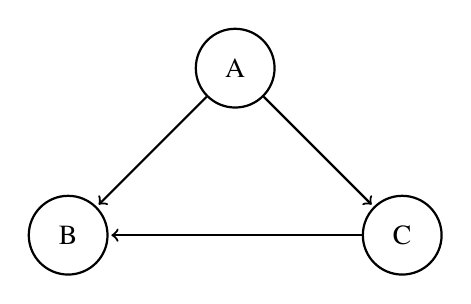
\begin{tikzpicture}[->,shorten >=1pt,auto,node distance=3cm,
         thick,main node/.style={circle,draw,minimum size=1cm,inner sep=0pt]}]

     \node[main node] (A) {A};
     \node[main node] (B) [below left of=A]  {B};
     \node[main node] (C) [below right of=A] {C};

     \draw[->] (A) -- (B);
     \draw[->] (A) -- (C);
     \draw[->] (C) -- (B);
 \end{tikzpicture}
 \end{minipage}
 \begin{minipage}{0.4\columnwidth}
 \centering
 \begin{tabular}{cccc}
   & A   &  B  & C   \\
 \toprule
 A & 0.0 & 0.1 & 0.9 \\
 B & 0.1 & 0.0 & 0.9 \\
 C & 0.5 & 0.5 & 0.0 \\
 \bottomrule
 \end{tabular}

 \end{minipage}

 \caption{Example of Markov Chain represented as a directed graph with its respective probability table.}
 \label{fig:markov_chain}
\end{figure}

Markov chains can be derived manually with the support of music theory  or learned from a corpus of music pieces. In both cases, one has to define how to encode music symbols into a sequence of states \cite{ames1989markov}. To learn a Markov chain from a corpus, one can count, for each state $s_1$ in the corpus, the number of times $s_1$ appears after each other state $s_2$. The transition probability table can then be constructed by normalizing these counts with the total number of transitions in the corpus.
The third and fourth movements of the \textit{ILLIAC Suite} are the earliest examples of
manually-designed Markov chains, while \citet{brooks1957} presented one of the first examples inferred from a corpus of music. \citet{brooks1957} experimented with different orders of Markov chains where each state represents a pitch class. The probability tables of these chains were learned from 37 common meter ($\frac{4}{4}$) hymn tunes (monophonic). While Markov chains designed manually by composers
worked well for specific compositional tasks \cite{tipei1975mp1, jones1981compositional, langston1989six},
those learned from a corpus, in practice, can capture only short-term dependencies in music
\cite{moorer1972music}. Moreover, low order chains typically generate unmusical compositions that
wander aimlessly, while high order ones tend to repeat segments from the corpus and are
very expensive to train \cite{moorer1972music}.

Markov chains can also be used to evaluate music generated by other methods. Given a sequence of states representing a piece of music, one can evaluate this piece with the joint probability of the sequence as given by the Markov chain. Thus, the higher the probability, the better the music. This approach was used by \citet{lo2006evolving}. They trained a Markov chain with classical music pieces and used it to calculate the fitness of candidate solutions of an EA. Each solution in the EA represents a melody encoded as a sequence of pitch numbers as defined by the MIDI format.

Most methods presented in this section require manually designed musical models (or rules) to manipulate or evaluate music. Although music theory formalizes several aspects of music analysis and composition, designing computational music models for AMC is still very challenging, given that music composition is a task that involves human creativity. Some of the presented methods, such as generative grammars and Markov models, can infer composition rules from a music corpus. However, in practice, they have limited performance in terms of music quality. Deep learning is a modern approach to AI, where neural networks are trained to perform various tasks. Recently, the AI research community has drawn substantial attention to this approach due to the impressive results that it has been achieving in different problems (e.g., image classification, speech recognition, and machine translation) \cite{lecun2015deep}. These results also motivated AMC researchers to explore deep learning algorithms for music composition \cite{briot2017deep}. The next chapter presents a detailed discussion on how (deep) neural networks can learn music models from a symbolic music corpus.


\chapter{Deep Learning for Algorithmic Music Composition}
\label{ch:ml}
\textit{Deep Learning} is a class of \textit{Machine Learning} (ML) algorithms based on \textit{Neural Networks} (NNs) with multiple layers that progressively extract higher-level features from raw data (e.g. text, images, audio, video, etc) \cite{goodfellow2016deep}. As ML algorithms, deep neural networks are used to learn different tasks from examples without being explicitly programmed to do so, including \textit{supervised learning} tasks, \textit{unsupervised learning} tasks, and \textit{reinforcement learning} tasks. In a \textit{supervised learning} task, pairs $(x^i,y^i)$ of inputs $x^i$ and target classes (also called labels) $y^i$ are provided by a dataset as training examples. The NN then is \textit{trained} to learn a function that maps the input examples into the target classes. The learned function is typically used to perform predictions (e.g. classification) on examples that the NN has not seen during training. Supervised learning is typically divided into \textit{binary} and \textit{multiclass} problems. In binary problems, a given input $x^i$ can have one of two possible labels $y^i = \{0, 1\}$. In multiclass problems, the label $y^i = \{0, 1, \cdots, L\}$. can take one of $L > 2$ values. A classic example of a binary problem is email spam detection (spam or not). A popular example of a multiclass problem is classifying images of handwritten digits \cite{lecun1998gradient}. In an unsupervised learning problem, only the inputs $x^i$ are given in the dataset, and the NN is trained to learn internal patterns in the data. These learned patterns can be used for different purposes such as clustering, transfer learning, and generative modeling \cite{bengio2012unsupervised}. In reinforcement learning, the NN is trained to learn an agent that can take optimal actions in an environment according to a \textit{reward function}.

Most modern music composition systems are designed as unsupervised learning tasks, where a deep NN has to learn relationships from music structures (e.g. notes, chords, melodies) represented in symbolic format. Formally, these NNs are \textit{generative models}, i.e. a model that captures a probability distribution $P(X)$ from a given dataset $X$. Inspired by the great results that deep learning has achieved in NLP, music generative models are typically designed as a neural \textit{language model} (LM). In NLP, a LM is a conditional probability $P(x_t|x_1, \cdots, x_{t-2}, x_{t-1})$ of the next word $x_t$ given a context with the $t$ previous words $\{x_1, \cdots, x_{t-2}, x_{t-1}\}$ of a sentence. One can create a LM $P$ from examples $(x_t, x_{t+1})$ by training a NN to predict the next word $x_{t+1}$  from the current word $x_t$. A NN trained this way can generate new sentences by sampling from the learned distribution $P$. Considering that music is a sequence of musical ``words'' (e.g., notes, chords, sections), one can train a neural LM to compose music by (a) creating a dataset of symbolic music, (b) defining the architecture of the NN to learn the conditional probability $P$, and (c) sampling tokens from the learned conditional probability $P$. The remainder of this chapter discusses different approaches for these three steps.

% Representation and Datasets
\section{Symbolic Music Representation}

Symbolic music representation refers to using high-level symbols such as tokens, events, or matrices as a representation for music modeling. The advantage of symbolic music representation over audio music representation is that the former incorporates higher-level features such as structure, harmony, and rhythm directly within the representation itself, without the need for further preprocessing. There are many formats to represent symbolic music in computers, but the most common ones are MIDI and Piano Roll.

\subsection{MIDI}
MIDI is a standard protocol for interoperability between various electronic instruments, devices, and software. A MIDI file represents a music piece as a series of messages that specify real-time note performance data and control data. The two most important messages for music LMs are the following:

\begin{itemize}
  \item NOTE\_ON: this message is sent when a note starts, and it has three parameters:
  \begin{itemize}
      \item \textit{Channel number}: indicates the instrument track with an integer $0 \leq i \leq 15$
      \item \textit{Note number}: indicates the note pitch with an integer $0 \leq p \leq 127$
      \item \textit{Note velocity}: indicates how loud the note is played with an integer
      $0 \leq v \leq 127$
  \end{itemize}

  \item NOTE\_OFF: this message is sent when a note ends, and it has the same three parameters as the
  NOTE\_ON message. In this case, the velocity parameter indicates how fast the note is released.
\end{itemize}

Note events are organized into a stream format called \textit{track chunk}, which specifies the timing information of each note event with a delta time value. A delta time value represents either the time of the note event in a relative metrical time (number of ticks from the beginning) or absolute time. In the relative metrical format, a reference called \textit{division} is defined in the file header to set the number of ticks per quarter note. Table \ref{tab:midi} shows an example of a MIDI \textit{track chunk} encoded in a readable format, where the time division has been set to 384, i.e. 384 ticks per quarter note.

\begin{table}[h]
    \centering
    % \setlength{\tabcolsep}{4pt}
    \begin{tabular}{llllll}
        \textbf{Delta time} & \textbf{Event Type} & \textbf{Channel} & \textbf{Pitch} & \textbf{Velocity} \\
        96  & NOTE\_ON  & 0 & 60 & 90 \\
        192 & NOTE\_OFF & 0 & 60 & 0  \\
        192 & NOTE\_ON  & 0 & 62 & 90 \\
        288 & NOTE\_OFF & 0 & 62 & 0  \\
        288 & NOTE\_ON  & 0 & 64 & 90 \\
        384 & NOTE\_OFF & 0 & 64 & 0
    \end{tabular}
    \caption{Example of MIDI file encoded in a readable format.}
    \label{tab:midi}
\end{table}

% To use MIDI formats with LMs, one has to create a vocabulary of symbols that represent
% note events and their attributes. This vocabulary is then used to encode the stream of events
% in a given set of MIDI files as a sequence of symbols.
% There are many different ways to do that with smaller or bigger vocabularies.
% The pros and cons of some of the common approaches are discussed later in this chapter.

\subsection{Piano Roll}
Another very common format of symbolic music is the \textit{piano roll}. This format is inspired by classic automated pianos that play pieces without a human performer by reading music from a continuous roll of paper with perforations punched into it. Each perforation automatically triggers a note, where the perforation location defines the note pitch, and the perforation length defines the note duration. In a modern piano roll, music is divided into discrete time steps forming a grid where the x axis represents time, and the y axis represents pitch. The values $0 \leq v \leq 127$ in the grid represent the velocity of the notes. Figure \ref{fig:piano_roll} shows an example of modern piano roll representation.

\begin{figure}[!h]
 \centering
 \includegraphics[width=\columnwidth]{imgs/background/piano_roll.jpg}
 \caption{Example of music represented in a piano roll format.}
 \label{fig:piano_roll}
\end{figure}

% Using a piano roll representation with LMs also requires creating a
% vocabulary of symbols to represent notes and their attributes
% (duration and velocity). However, the sequence of symbols is defined
% by the time steps in the piano roll, instead of the stream of events
% in the MIDI representation.

The MIDI representation can be mapped to a piano roll by sampling time steps with a given frequency (e.g. every eighth note). Because of this property, most datasets of symbolic music organize pieces in a collection of MIDI files. For example, the \textit{MAESTRO} dataset \cite{hawthorne2018enabling} is composed of about 200 hours of virtuosic piano performances of classical music pieces captured from the International Piano-e-Competition \cite{yamahaEPiano} in MIDI format aligned with audio waveforms. The \textit{Lakh} \cite{raffel2016learning} dataset is a collection of 176,581 unique MIDI files from various music genres (mostly pop music) scraped from publicly available sources on the internet, where 45,129 of them have been matched and aligned to entries in the \textit{Million Song Dataset} \cite{bertin2011million}. \textit{Piano midi.de} is a dataset of classical piano pieces from a wide variety of composers recorded in MIDI with a digital piano. JSB Chorales \cite{boulanger2012modeling} contains the entire corpus of 382 four-part harmonized chorales by J. S. Bach.

MIDI and piano roll are the most common formats used to represent symbolic music. However, there are also other formats that have been used in the AMC literature. For example, the ABC notation \cite{walshaw1993abc2mtex} is a text-based music notation system popular for transcribing,
publishing and sharing folk music. MusicXML \cite{good2001musicxml} is a markup language that has been designed to facilitate the sharing, exchange, and storage of scores by musical software systems.

To use any of these symbolic music representations with LMs, one has to define a vocabulary that encodes music data into music symbols. These symbols will be used to create sequences that represent music pieces. For example, in a MIDI representation, one has to map the note events into tokens and use the delta-time information from the \textit{track chunks} to define the order of symbols that will form the music pieces. In a piano roll representation, one has to map the vertical axis (pitch) into tokens and process the piano roll grid either horizontally or vertically to define the order of the tokens. To be processed by NNs, each symbol in the vocabulary has to be mapped into a vector. Traditionally, these symbols are mapped using \textit{one-hot} encoding, where each symbol is given an index $i$ and is represented by a vector $v = [v_1, v_2, \cdots, v_n]$ where only $v_i = 1$ and all the other dimensions $v_{j \neq i} = 0$. In the one-hot encoding, $n$ is the number os symbols in the vocabulary.

\section{Neural Networks}

% With a dataset of music represented in a symbolic format (MIDI, piano roll, etc.),
% one can train a ML model to learn a LM that can generate music.
% In early examples, LMs were typically implement with Markov chains and
% recently LMs are more commonly modeled with artificial neural networks.
Artificial Neural Networks, or simply Neural Networks (NNs), interconnect a number of simple processing units called \textit{neurons} to learn a function from training examples. These neurons are typically organized into layers. Neurons might be connected to several other neurons in the layer before it, from which it receives data, and several neurons in the layer after it, to which it sends data. NNs can be defined with different \textit{architectures}, i.e. with a different number of layers (\textit{depth}) and different layouts of neuron connections. The first layer of the network is called the \textit{input layer}, and the last one is called the \textit{output layer}. All the intermediate layers are called \textit{hidden layers}. Each neuron in the hidden or output layers takes as input a vector $x = [x_1, x_2, \cdots, x_n]$ of incoming connections from the previous layer and assigns a weight vector $w = [w_0, w_1, \cdots, w_n]$ to these connections. In its most basic form, the neuron first applies a linear transformation $z = w \dot x + b$ to the inputs $x$, where $b$ is an extra weight called \textit{bias} that is not tied to any neuron of the previous layer. The neuron then uses a nonlinear function called \textit{activation function} $f$ to map the linearly transformed inputs $z$ into an output $\hat{y}$.
Figure \ref{fig:nn} shows a three-layer\footnote{Typically, the input layer is not considered when counting the depth of the NN.} NN called \textit{feedforward} network or \textit{multilayer perceptron} (MLP),
with the computation performed by each layer highlighted besides them. The bias terms have been removed for clarity.

\begin{figure}[!h]
\centering
\includegraphics[width=0.7\columnwidth]{imgs/background/ann.png}
\caption{Diagram of a feedforward neural network \cite{lecun2015deep}.}
\label{fig:nn}
\end{figure}

The number of neurons per layer, i.e. the \textit{layer size}, and the layers' activation functions depend on the task that the NN is learning. In traditional supervised problems, the input layer size is defined by how the input examples are represented and the output layer size by the number of classes in the problem. For example, consider a handwritten digits classification problem in which each handwritten digit is stored in a 28x28 grayscale image. The goal is to classify the images into one of the ten digits (zero to nine). The input layer size is 784 neurons, one for each pixel in the image. The output layer size is 10 neurons, one for each class. The size of the hidden layers is defined arbitrarily and should be controlled to optimize the performance (e.g. prediction accuracy) of the network.

In \textit{multiclass} problems, such as the handwritten classification, the \textit{softmax} activation function is used in the output layer to create a probability distribution over the classes. Thus, the NN predicts the class with maximum probability. In \textit{binary} problems, the \textit{logistic} activation function is typically used to map the output layer into a single output $0 \leq \hat{y} \leq 1$. The NN predicts $1$ if $\hat{y} > 0.5$ and $0$ otherwise. The activation functions used in the hidden layers are decided arbitrarily as well, and they also affect the performance of the NNs. Three of the most common activation functions used in the hidden layers are: \textit{logistic}, \textit{tanh}, and \textit{ReLu}. Table \ref{tab:activation} formally describes each of these functions.

\begin{table}[h]
    \centering
    % \setlength{\tabcolsep}{4pt}
    \begin{tabular}{lll}
        \textbf{Name} & \textbf{Function} \\
        Logistic (sigmoid) & $\sigma(x) = \frac{1}{1 + e^{-x}}$ \\
        Hyperbolic tangent (tanh) & $tanh(x) = \frac{e^x - e^{-x}}{e^x + e^-x}$ \\
        Rectified linear unit (ReLu) & $relu(x) = max(0, x)$ \\
        Softmax & $softmax(x) = \frac{e^{x_i}}{\sum_{j=1}^{J} e^{x_j}}$ \\
    \end{tabular}
    \caption{A list of common activation functions in the hidden layer.}
    \label{tab:activation}
\end{table}

NNs are typically trained with some variation of the \textit{gradient descent} (GD) algorithm, which optimizes the weights $W^i$ and $b^i$ of all layers $i$ of the network to minimize a given \textit{loss function} $J(W,b)$. The loss function depends on the task being modeled by the NN. However, in supervised learning, one of the most common losses is the \textit{cross-entropy}, which measures the difference between the training data distribution and the distribution modeled by the NN. Equation \ref{eq:cross_entropy} formally defines the cross-entropy loss for a single example, where $y_c$ is the target label for the class $c$, $\hat{y}_c$ is the output predicted by the $NN_{W^i,b^i}$ with parameters $W$ and $b$ for class $c$, and $C$ is the number of classes in the prediction task.
\begin{equation} \label{eq:cross_entropy}
\begin{split}
    J(W,b) = -\sum_{c=1}^{C} y_clog(\hat{y}_c)
\end{split}
\end{equation}

% In its basic formulation, GD uses the average loss of the entire dataset to update the weights $W^i$ and $b$ of the NN $N_{W,b}$.
As shown in Algorithm \ref{alg:grad_desc}, GD works by iteratively taking steps in the opposite direction of the gradient of the loss function with respect to all weights. For a given number of iterations called \textit{epochs}, GD (line \ref{line:grad}) computes the gradient vector of the loss function $J(W,b)$ for the entire training dataset and (line \ref{line:update}) updates the parameters $W^i$ and $b^i$ in the opposite direction of the gradient. The \textit{learning rate} $\alpha$ is a parameter that controls the size of the training step. Computing the gradient vector (line \ref{line:grad}) requires calculating the partial derivatives of the loss function with respect to all the weights in the NN. This calculation is typically performed by an algorithm called \textit{backpropagation}, which uses the chain rule to compute the gradient one layer at a time, iterating backwards from the output layer to avoid redundant calculations of intermediate terms in the chain rule.

\begin{algorithm}[t]
\caption{Gradient Descent}
\label{alg:grad_desc}
\begin{algorithmic}[1]
\REQUIRE Dataset $(X, Y)$, a loss function $J(W,b)$, a NN $N_{W^i,b^i}$ with
parameters $W^i$ and $b^i$, the number of epochs $e$ and the learning rate $\alpha$.
\ENSURE Updated parameters $W^i$ and $b^i$ of all layers $i$.
\FOR{$i \gets 1$ \TO $e$ }
       \STATE $\partial W^i \gets \frac{\partial J}{\partial W^i}$, $\partial b^i \gets \frac{\partial J}{\partial b^i}$ \label{line:grad}
       \STATE $W^i \gets W^i - \alpha \, \partial W^i$, $b^i \gets b^i - \alpha \, \partial b^i$ \label{line:update}
\ENDFOR
\end{algorithmic}
\end{algorithm}

Calculating the gradients for the whole dataset to perform just one update can be very slow or intractable for datasets that do not fit in memory. \textit{Stochastic Gradient Descent} (SGD) is a variation of GD that solves this problem by splitting the training data into sets called \textit{batches} of size $N$ and performing a parameter update for each one of them.  Although SGD supports training with very large datasets, it introduces convergence issues due to the variance in the frequent updates that cause the value of the loss function to fluctuate. \textit{Adaptive Moment Estimation} (Adam) is a recent variation of SGD that mitigates this problem by having a learning rate per per-parameter and separately adapting them during training \cite{kingma2014adam}. In practice, most practitioners use the Adam optimizer, given that successfull NNs typically require large datasets that do not fit in memory\footnote{The term \textit{big data} is typically used to refer to these very large datasets.}.

\subsection{Recurrent Neural Networks}
\label{sec:rnns}

\textit{Recurrent Neural Networks} (RNNs) are an important architecture for AMC because they were specifically designed to model sequential data. RNNs process sequences $x = [x_1, x_2, \cdots, x_t]$ step-by-step by keeping an internal state $h_t$ that is updated every step. Each element $x_i$ is a vector representing a token (e.g. words in English or pitch classes in western music) traditionally encoded as a one-hot vector. Figure \ref{fig:rnn} shows an abstract diagram of an RNN.

\begin{figure}[!h]
\centering
\includegraphics[width=0.9\columnwidth]{imgs/background/rnn.png}
\caption{Diagram of a RNN \cite{olah2015understanding}.}
\label{fig:rnn}
\end{figure}

On the left-hand side, the RNN is shown with an input layer that passes a symbol $x_t$ to a stack of hidden layers $A$ that updates $h_t$. A loop in the hidden layers allows information to be passed from one step of the network to the next. The right-hand side shows an unrolled version of the same RNN. The output layer of the network is omitted from the diagram because RNNs can produce multiple outputs, one per time step or one single output at the very last time step. This configuration depends on the problem. However, the output layer maps a current hidden state $h_t$ to an output vector $y$.

Two of the most simple types of RNNs are the \textit{Elman} and \textit{Jordan} networks. They are RNNs with three layers: an input layer, a single hidden layer, and an output layer. In these networks, an output $y_t$ is produced for each time step $t$. Equation \ref{eq:elman} and Equation \ref{eq:jordan} formally describe these networks, respectively, where $W_{xh}$, $W_{hh}$ and $W_{hy}$ are weight matrices and $\sigma$ are activation functions. The matrices $W_{xh}$, $W_{hh}$ represent the weights of the hidden layer, and the matrix $W_{hy}$ represent the weights of the output layer. The weights $W_{hh}$ are called context units.
\begin{align}
\begin{split}
    h_t &= \sigma(W_{xh}x_t + W_{hh}h_{t-1}) \\
    y_t &= W_{hy}h_t
\end{split}
\label{eq:elman}
\end{align}
\begin{align}
\begin{split}
    h_t &= \sigma(W_{xh}x_t + W_{hh}y_{t-1}) \\
    y_t &= W_{hy}h_t
\end{split}
\label{eq:jordan}
\end{align}

These two networks are very similar. The main difference is that the context units are fed from the output layer instead of the hidden layer. Todd \cite{todd1989connectionist} presented one of the first applications of NNs for music composition: a \textit{Jordan} network designed to generate melodies (monophonic). The input of this network is a melody encoded as a sequence of pitch classes (e.g. \textit{CDEGFEDF}), and the output is a single pitch. This network was trained to reconstruct given example melodies. Each melody contributed to $t$ training steps, where $t$ is the size (number of pitches) of the melody. At every training step $t$, the current example melody is given as input, and the network error is calculated by comparing the network output $y_t$ with the respective pitch $x_t$ of the input melody. After training, one could give new melodies as input to the network, which would create new melodies interpolating between the ones used during the training phase. Duff \cite{duff1989backpropagation} published another early example that is similar to the work of Todd \cite{todd1989connectionist}, but Duff encoded each melody as a sequence of note intervals\footnote{The distance in pitch between two notes.} instead of pitch classes.

One of the major problems of RNNs consists of modeling long-term dependencies between symbols in a sequence. Modeling long-term dependency consists of creating an RNN capable of considering previous symbols that are distant from the one that is being predicted. In practice, simple RNNs are unable to connect the information between symbols that are very far from each other \cite{bengio1994}. In music, modeling long-term dependencies is critical to generate long complete pieces with coherent form.

\subsection{Long Short-Term Memory Networks}
\label{sec:lstm}
% LSTM and GRU

Long Short-Term Memory (LSTM) network \cite{hochreiter1997long} is a special type of RNN explicitly designed to solve the problem of simple RNNs with long-term dependencies. As shown in Figure \ref{fig:rnn}, RNNs have the form of a chain of repeating stacks of layers $A$. LSTMs follow the same structure, but the repeating module performs different computations. Figure \ref{fig:lstm} shows a diagram of a LSTM. A single LSTM module $t$ is composed of an extra state $C_t$ called \textit{cell state}, which is responsible for carrying information through the entire LSTM network. The float of information in the cell state is controlled by four \textit{gates}: an input gate $i_t$, an output gate $o_t$ and a forget gate $f_t$. These gates facilitate the cell to remember or forget information for an arbitrary amount of time.

\begin{figure}[!h]
\centering
\includegraphics[width=0.9\columnwidth]{imgs/background/lstm.png}
\caption{Diagram of a LSTM \cite{olah2015understanding}.}
\label{fig:lstm}
\end{figure}

Equation \ref{eq:lstm} formally defines the computation performed in each LSTM module, where $W_f$, $W_i$, $W_c$, and $W_o$ are weight matrices, $[h_{t-1}, x_t]$ is the the hidden state vector $h_{t-1}$ concatenated with the input vector $x_t$, and $\tilde{C}_t$ is the candidate vector to added to the cell state.
\begin{equation} \label{eq:lstm}
\begin{split}
    f_t &= \sigma(W_f[h_{t-1}, x_t]) \\
    i_t &= \sigma(W_i[h_{t-1}, x_t]) \\
    \tilde{C}_t &= tanh(W_c[h_{t-1},x_t]) \\
    C_t &= f_t * C_{t-1} + i_t * \tilde{C}_t \\
    o_t &= \sigma(W_o[h_{t-1}, x_t]) \\
    h_t &= o_t * tanh(C_t)
\end{split}
\end{equation}

Each gate $i_t$, $o_t$, and $f_t$ have the exact same equation, just with different weight matrices ($W_i$, $W_o$ and $W_f$, respectively). The cell state $C_t$ combines the input and forget gates to control the amount of information that will be included from the input versus the amount of information that will be forgotten from the current cell state, respectively. The output gate controls the parts of the cell state that will be included in the final hidden state $h_t$. Modern RNNs (including LSTMs) typically have an extra hidden layer that is added before any other hidden layer to transform the one-hot input vectors $x_t$ into \textit{embeddings}. In NLP, a word \textit{embedding} is a learned representation for text where words that have the same meaning have a similar representation. The \textit{embedding} layer learns a dense vector representation of arbitrary dimension from the sparse one-hot representation of the symbols in the vocabulary.

% TODO: Add figure with embedding example
% TODO: bidirectional LSTMs

Early RNNs were not necessarily trained as LMs (see Section \ref{sec:rnns}), but most modern LSTMs compose music as a LM. To learn a LM from an LSTM, one has to map the output at each time step $\hat{y_t}$ to a probability distribution over the symbols in the defined music vocabulary. This is normally done with a \textit{softmax} activation function in the output layer. The LSTM is then trained with mini-batch gradient descent to predict the next symbol $y_{t_1}$ given the current symbol $y_t$ from music pieces given as training data. Many recent deep learning approaches used LSTMs to model music generation with LMs \cite{briot2017deep}. For example, Lyu et. al. \cite{lyu2015modelling} combined an LSTM with another type of neural network called Restricted Boltzman Machine (RBM) to generate polyphonic music with different musical styles. They experimented with both the Musedata and the JSB Chorales \cite{boulanger2012modeling}. The pieces were encoded as a sequence of pitch numbers temporally aligned on an integer fraction of a quarter note. This encoding system only considered pitch and duration and hence did not considered dynamics information (e.g. note velocity).

BachBot \cite{liang2017automatic} uses a deep LSTM to generate polyphonic in the style of Bach’s chorales. BachBot was trained with the JSB Chorales dataset, where each chorale was encoded with a sequence of sixteenth-note frames. Each frame consisted of four tuples (Soprano, Alto, Tenor, and Bass), and each tuple in the form (\textit{pitch}, \textit{tie}), where \textit{pitch} represents a MIDI pitch and \textit{tie} is a boolean value that distinguishes whether a note is tied with a note at the same pitch from the previous frame or is articulated at the current time step. This encoding system also did not consider dynamics information. Oore et al. \cite{oore2017learning} propose one of the first methods that can generate music with dynamics. They trained an LSTM with a new representation that supports tempo and velocity events from MIDI files. This model was trained on the MAESTRO \cite{hawthorne2018enabling}. With this new representation and dataset, Oore et al. \cite{oore2017learning} generated more human-like performances when compared to previous models.

\subsection{Transformers}

\textit{Transformer} \cite{vaswani2017attention} is a modern architecture for sequence modeling based on \textit{attention} mechanisms, as opposed to recurrent layers. In NLP, an attention mechanism is a part of a neural architecture that enables highlighting relevant words of the input sequence dynamically. Instead of keeping an internal hidden state that is updated at each time step like RNNs, transformers process entire sequences associating an \textit{attention} score to each token that determines how much that token contributes to the output of the network. Because transformers process tokens in parallel, they can take advantage of the parallel computing offered by GPUs, and hence transformers can be trained considerably faster than LSTMs \cite{vaswani2017attention}. One drawback of the transformers is that they can only process sentences with a fixed size instead of LSTMs that can process sentences of any size.

Transformers were originally designed in the context of \textit{machine translation}, an NLP task that consists of translating a sequence from one language (e.g. English) to another (French). Machine translation is a \textit{sequence-to-sequence} problem, where a sequence input $x$ has to mapped into an output sequence $y$. NNs designed for machine translation normally have a \textit{encoder-decoder} structure. The first part of the network, called the \textit{encoder}, takes a sequence as input $x$ and outputs a vector representation $e$ (called \textit{encodings}) of the input $x$. The second part, called \textit{decoder}, takes the encodings $e$ as input and outputs a sequence $y$. As shown in Figure \ref{fig:transformer}, the transformer has an encoder-decoder structure (the encoder is showed on the left side and the decoder on the right side). The transformer takes as input a sentence typically encoded as one-hot vectors and transforms it into two sequences: a sequence of \textit{word embeddings} and a sequence of \textit{positional embeddings}. The former is a dense vector representation of words learned from the sparse one-hot input. The latter is also a dense vector representation but learned from the position (indices) of the words in the input sentence. The transformer adds the input embeddings and positional encodings together and passes the result through the encoder, followed by the decoder.

% TODO: Add figure with input + positional embedding example

\begin{figure}[!h]
 \centering
 \includegraphics[width=0.5\columnwidth]{imgs/background/transformer.png}
 \caption{Diagram of a Transformer \cite{vaswani2017attention}.}
 \label{fig:transformer}
\end{figure}

The encoder converts the (input + position) embeddings $e$ into \textit{encodings} with a stack of $n$ identical layers called \textit{transformer blocks}. Each transformer block has two layers: a \textit{multi-head attention layer} and a fully connected \textit{feedforward layer}. A residual connection \cite{he2016deep} is applied around each of the two layers, followed by a layer normalization \cite{ba2016layer}. A residual connection is a connection between non-contiguous layers. A layer normalization is an extra layer that normalizes the activations of the previous layer, i.e. it applies a transformation that maintains the mean activation within each example close to 0 and the activation standard deviation close to 1.

The most important part of the transformer architecture is the \textit{multi-head attention layer}, which computes a score matrix $Z$ from the embeddings $e$, where the scores in $Z$ represent the relationship between different words in the input sentence. For example, consider the sentence ``The animal didn't cross the street because it was too tired.''. In this sentence, the word ``it'' is related to ``animal'', and so when the transformer is processing the word ``it'', self-attention allows it to associate ``animal'' with ``it''. Figure \ref{fig:attn} shows the encoder self-attention distribution for the word ``it'' in this example.

\begin{table}[h]
    \centering
    \includegraphics[width=0.5\columnwidth]{imgs/background/attn.png}
    \caption{The encoder self-attention distribution for the word ``it'' in the sentence
    ``The animal didn't cross the street because it was too tired.'' \cite{vaswani2017attention}.}
    \label{fig:attn}
\end{table}

The score matrix $Z$ is computed similarly to a dictionary lookup: it takes a \textit{query} matrix $Q$, a \textit{key} matrix $K$, and a \textit{value} matrix $V$, and outputs a weighted sum of the values that correspond to the keys that are most similar to the query. One of the most common self-attention mechanisms in a transformer neural network is the scaled dot-product attention, which is shown in Equation \ref{eq:attn}. The matrices $Q$, $K$, and $V$ are created by packing the embeddings $e$ of all the words in the input sentence into a matrix $E$, and multiplying it by the weight matrices $W_q$, $W_k$ and $W_v$ that are learned during training.

\begin{equation}\label{eq:attn}
\begin{split}
    Z = Attention(Q, K, V) &= softmax(\frac{QK^T}{\sqrt{d_k}})V \\
    Q &= E * W_q \\
    K &= E * W_k \\
    V &= E * W_v
\end{split}
\end{equation}

The decoder is similar to the encoder, but it has an extra attention layer added before the other two to perform multi-head attention over the target output sentence $y$. This extra layer uses a mask to ensure that the predictions for position $i$ can depend only on the known outputs at positions less than $i$. The output of the decode is a linear layer followed by a softmax activation.

One can take the decoder portion of the transformer to train a LM capable of generating sequences such as text or music similar to a LSTM LM (see Section \ref{sec:lstm}). Equation \ref{eq:transformer} formally defines a decoder-based transformer LM, where $x = [x_1, x_2, \cdots, x_t]$ is the input sequence, $n$ is the number of layers, $W_i$ is input embedding weight matrix, and $W_p$ is the position embedding weight matrix.

\begin{equation}\label{eq:transformer}
\begin{split}
    h_0 &= W_ix + W_p \\
    h_l &= transformer\_block(h_{l-1}) \forall i \in [1,n] \\
    P(u) &= softmax(h_nW_e^T)
\end{split}
\end{equation}

Transformers are currently the state-of-the-art of both natural and music language modeling. Radford et. al. \cite{Radford2018, radford2019language} proposed a series of models called GPT (General Pre-trained Transformer), GPT-2, and GPT-3 that used only the decoder part of the original transformer to create a model of natural language. Radford et. al. showed that besides generating long coherent sequences of text, pre-trained GPT models can be fine-tuned with a simple extra linear layer to perform specific NLP tasks (e.g. commonsense reasoning, question answering, summarization, and others) with state-of-the-art performance. Pre-training consists of training the GPT model as a (unsupervised) LM with a huge general dataset (e.g. Wikipedia). Fine-tuning is performed by adding an extra linear layer to the pre-trained transformer and training this layer with a smaller dataset explicitly created for the task (supervised).

Music Transformer \cite{huang2018music} is one of the first decoder-transformer to generate music. It uses a new relative attention mechanism that improves memory consumption of the original decoder, and hence it can process longer sequences. Music Transformer achieves state-of-the-art performance on the MAESTRO dataset \cite{hawthorne2018enabling}. Donahue et. al. \cite{donahue2019lakhnes} showed that a decoder-transformer could also compose multi-instrument scores by training it with the NES MDB \cite{donahue2018nesmdb} dataset. Donahue et al. improved the performance of their model with a pre-training procedure similar to Radford et al. \cite{Radford2018}. The transformer was first pre-trained with the diverse Lakh dataset (multiple instruments) and then fine-tuned with NES-MDB (four instruments). They manually defined a mapping between the instruments from the two datasets. Pop Music Transformer \cite{huang2020pop} is a transformer model with a specialized music representation to compose pop piano music. It was shown to generate a better rhythmic structure than previous transformer models.

% TODO: Convolutional Neural Networks

\subsection{Variational Autoencoders}

\textit{Variational Autoencoders} (VAEs) \cite{kingma2013auto} are another modern architecture that can be used to generate music. VAEs are different from RNNs and Transformers because they were not specifically designed to model sequences. Instead, they are generative models that can potentially learn to represent any data. VAEs have an architecture similar to a traditional \textit{Autoencoder}, which is an encoder-decoder NN used to learn efficient encodings of unlabeled data (unsupervised learning). Figure \ref{fig:ae} shows a diagram of an autoencoder.

\begin{figure}[!h]
 \centering
 \includegraphics[width=0.8\columnwidth]{imgs/background/autoencoder.png}
 \caption{Diagram of an Autoencoder \cite{rocca2019understanding}.}
 \label{fig:ae}
\end{figure}

An autoencoder builds a latent space of a dataset $X$ with an encoder network $e$ by learning to compress each example $x$ into a vector $z$ and then reproducing $x$ from $z$ with a decoder network $d$. A key component of an autoencoder is the bottleneck introduced by making the vector have fewer dimensions than the input data itself, which forces the model to learn a compression scheme. During training, the autoencoder ideally distills the qualities that are common throughout the dataset. As shown in Figure \ref{fig:ae_sampling}, one can use an autoencoder as a generative model by sampling random vectors from the latent space learned by the encoder and using the trained decoder to build the output from the sampled vector.

\begin{figure}[!h]
 \centering
 \includegraphics[width=0.8\columnwidth]{imgs/background/ae_sampling.png}
 \caption{Sampling from the latent space built by an Autoencoder \cite{rocca2019understanding}.}
 \label{fig:ae_sampling}
\end{figure}

One limitation of the autoencoder is that it often learns a latent space that is not continuous\footnote{Two close points in the latent space should yield similar outputs when decoded.} nor complete\footnote{Any point sampled from the latent space should yield a ``meaningful'' output when decoded}. This means that if one decodes a random vector sampled from the learned latent space, it might not result in a realistic output. VAEs solve this problem by encoding the dataset $X$ as a probability distribution over the latent space instead of a single vector $z$. Typically, this distribution is assumed to be a multivariate normal distribution $N(\mu_x, \sigma_x)$. Figure \ref{fig:vae} shows a diagram of a VAE. The difference between autoencoders and VAEs is that the encoder of the VAE outputs two vectors $\mu_x$ and $\sigma_x$, instead of a single vector $z$. These two vectors represent the mean and standard deviation of a normal distribution $N$. The decoder samples a vector $z \sim N(\mu_x, \sigma_x)$ from the distribution $N$ and reconstructs the input $x$ from the sampled $z$ using the decoder $d$.

\begin{figure}[!h]
 \centering
 \includegraphics[width=0.8\columnwidth]{imgs/background/vae.png}
 \caption{Diagram of a Variational Autoencoder (VAE) \cite{rocca2019understanding}.}
 \label{fig:vae}
\end{figure}

MusicVAE \cite{Roberts2017} is one of the first examples of VAE applied to music generation. It start by splitting the input sequence $x$ in to $U$ non-overlapping subsequences $y_u$, such that $x = [y_1, y_2, \cdots, y_U]$. The encoder process the segmented input $x$ with a bidirectional LSTM network that outputs two hidden states $\overleftarrow{h_t}$ and $\overrightarrow{h_t}$ that are concatenated to form a final hidden state $h_t$. The final hidden state $h_t$ is fed into two fully connected layers to produce the latent distribution parameters $\mu$ and $\sigma$. The decoder is a novel hierarchical LSTM that takes the latent vector $z \sim N(\mu_x, \sigma_x)$ as input and first produces $U$ embedding vectors $c = [c_1, c_2, \cdots, c_U]$, one for each subsequence $y_u$. An LSTM called the \textit{conductor} produces these embedding vectors, where the hidden state is initialized by passing $z$ through a fully connected layer followed by a \textit{tanh} activation function. Once the conductor has produced the sequence of embedding vectors $c$, each one is individually passed through a shared fully connected layer followed by a tanh activation to produce initial states for a final decoder LSTM. The decoder RNN then autoregressively produces a sequence of distributions over output tokens for each subsequence $y_u$ via a softmax activation in the output layer. At each step of the final LSTM, the current conductor embedding $c_u$ is concatenated with the previous output token to be used as the input.

MIDI-VAE \cite{brunner2018midi} uses a VAE to perform style transfer in polyphonic symbolic music. It works by separating a portion of the latent vector $z$ for style classification $z_s$, and another part $z_t$ to encode the characteristics of the music dataset. During generation, one can change the style $S_i$ of a given input piece $x$ to another style $S_j$ by passing a given input piece through the encoder to get $z$ and swapping the values of dimensions $z_s^i$ and $z_s^j$, and passing the modified latent vector through the decoder. Style labels can be music genres such as Jazz, Pop, and Classic; or composer names such as Bach or Mozart. VirtuosoNet \cite{jeong2019virtuosonet} is a VAE designed to generate piano performances with expressive control of tempo, dynamics, and articulations. The encoder is a hierarchical LSTM such that the input music is encoded on different levels: note, beat, and measure. The decoder renders musical expressions consistently over long-term sections by first predicting the tempo and dynamics in measure level and, based on the result, refining them in note level.

\subsection{Generative Adversarial Networks}

Similar to VAEs, \textit{Generative Adversarial Networks} (GANs) \cite{goodfellow2014generative} are powerful generative models that, in theory, can generate synthetic data in different domains. GANs are composed of two independent NNs: a \textit{generator} and a \textit{discriminator}. In its most basic form, the generator takes random noise as input and then transforms this noise into a fake example. The discriminator is a binary classifier that discriminates examples as \textit{fake} (0) or \textit{real} (1). The generator and the discriminator architectures depend on the data type (e.g. text, images, videos) that is being modeled. For example, Figure \ref{fig:gan} illustrates a GAN for handwritten digit generation. In this case, the random noise is a matrix $M$ representing a grayscale image. A simple way to generate such a matrix is to sample grayscale values between 0 (black) and 1 (white) from a uniform distribution. The generator transforms the random matrix $X$ into a fake handwritten digit normally using convolutional layers. The discriminator combines real and fake images to learn how to separate them between fake and real.

\begin{figure}[!h]
 \centering
 \includegraphics[width=\columnwidth]{imgs/background/gan.png}
 \caption{Diagram of a Generative Adversarial Network (GAN) \cite{silva2018intuitive}.}
 \label{fig:gan}
\end{figure}

Training a GAN consists of training the generator and the discriminator together
iteratively in alternating periods:

\begin{enumerate}
    \item The discriminator trains for one or more epochs.
    The discriminator is trained with a loss function that penalizes the discriminator for misclassifying a real instance as fake or a fake instance as real. The discriminator updates its weights through backpropagation from the discriminator loss through the discriminator network.

    \item The generator trains for one or more epochs.
    The generator is trained with a loss function that penalizes the generator for producing a sample that the discriminator network classifies as fake. In other words, the generator loss is computed via the discriminator. Thus, the generator updates its weights through backpropagation from the discriminator to the generator. It's important to highlight that only the generator weights are updated during generator training.
\end{enumerate}

The original GAN uses a single loss function called \textit{minimax loss} to train both the generator and the discriminator. Minimax loss is derived from the cross-entropy loss between the real and generated distributions. The generator tries to minimize this loss while the discriminator tries to maximize it. Equation \ref{eq:minimax_loss} formally defines the minimax loss, where $D(x)$ is the discriminator's estimate of the probability that real data instance x is real, $E_x$ is the expected value over all real data instances, $G(z)$ is the generator's output when given noise z, $D(G(z))$ is the discriminator's estimate of the probability that a fake instance is real, and $E_z$ is the expected value over all generated fake instances $G(z)$.

\begin{equation} \label{eq:minimax_loss}
    E_x[log(D(x))] + E_z[log(1 - D(G(z)))]
\end{equation}

During training, $G$ learns to generate fake data that resembles the original data, and $D$ learns to distinguish the generator's fake data from real data. The training process aims to have a generator $G$ that produces output that can fool the discriminator $D$. After training, one can generate new data points by sampling from different distribution points learned by $G$. This approach works well to generate continuous data such as images \cite{brock2018large}, but it has limitations in generating categorical data, especially in a sequential form such as text or music. Images can be represented by a continuous matrix $M$ and so applying transformations (e.g. $M' = M + 0.05$) to $M$ still results in defined images $M'$ that can be classified as real or fake by a discriminator. In sequential domains such as text and music, tokens are encoded using embedding vectors. Applying transformation to an embedding vector does not necessarily generate a valid token. For example, assume that the word ``university'' is represented by the vector $v = [0.44, 0.37, -0.28]$. If one applies the transformation $v' = v + 0.05$ to the original $v$, the new vector $v'$ not necessarily represent some word in the vocabulary. Therefore, updating the weights of $G$ with the gradients of the minimax loss might lead $G$ to generate invalid data. Another problem is that the discriminator can only provide feedback on entire sequences.

% TODO: Better summarize and correlate the different approaches
Different approaches have been proposed to solve these problems in the domain of symbolic music generation. For example, C-RNN-GAN \cite{yang2017midinet} generated polyphonic music as a series of note events by introducing some ordering of notes and using RNNs in both the generator and the discriminator. SeqGAN \cite{yu2017seqgan} combined GANs and reinforcement learning to generate monophonic music with an RNN generator and a CNN discriminator. MidiNet \cite{yang2017midinet} used GANs with conditional CNNs as both generator and the discriminator to generate melodies that follow a chord sequence given a priori, either from scratch or conditioned on the melody of previous bars. MuseGAN \cite{dong2018musegan} generates polyphonic music by encoding multi-track measures as a piano roll and also modeling both the generator and the discriminator as CNNs. Muhamed et al. \cite{muhamed2021symbolic} modeled both generator and the discriminator as transformers and used the Gumbel-Softmax trick \cite{jang2016categorical} to address the gradient problem of categorical generators.

\section{Decoding}

As discussed in the previous section, most neural generative models for AMC are based on architectures specially designed to model sequences: RNNs, LSTMs, and Transformers. Formally, these sequential models use a softmax activation function in the output layer to create a LM $L = P(x_t|x_1, \cdots, x_{t-2}, x_{t-1})$, where $\{x_1, \cdots, x_{t-2}, x_{t-1}\}$ is an input sequence and $x_t$ is the next token in that sequence. Typically, an \textit{autoregressive} strategy is used to generate music with $L$, i.e. to \textit{decode} the softmax output into a sequence of music tokens. Namely, one starts with a prior sequence of tokens $x = [x_1, x_2, \cdots, x_{t 1}]$, which are fed into $L$ to generate $L(x) = x_{t}$. Next, $x_{t}$ is concatenated with $x$ and the process repeats until a special end of-piece symbol is found or a given number of symbols are generated. As defined in Equation \ref{eq:autoregressive}, autoregressive generation assumes that the probability distribution of a sequence of tokens can be decomposed into the product of conditional next token distributions.

\begin{equation} \label{eq:autoregressive}
    P(x_t|x_1, \cdots, x_{t-2}, x_{t-1}) = \prod_{t=1}^{T} P(x_t|x_{1:t-1})
\end{equation}

Currently, most prominent \textit{autoregressive} strategies for music (and text) decoding are based either on \textit{sampling} or \textit{searching}. While sampling is well suited for creative tasks such as music composition, searching fits better generative problems where specific solutions are expected, such as machine translation.

\subsection{Top-k Sampling}

In its most basic form, sampling consists of randomly picking the next token according to the conditional probability distribution given by the LM: $x_t \sim P(x_t|x_{1:t-1})$. Figure \ref{fig:topk} shows and example where the prior is the sequence $x = [\textit{The}]$. In the first step, the word \textit{car} is sampled from the condition probability distribution $P(x_1 | \textit{The})$ and, in the second step, the word \textit{drives} is sampled from $P(x_2 | \textit{The}, \textit{car})$.

\begin{figure}[!h]
 \centering
 \includegraphics[width=0.9\columnwidth]{imgs/background/sampling.png}
 \caption{Example of sampling for text generation with prior $x = [\textit{The}]$ \cite{platen2020}.}
 \label{fig:topk}
\end{figure}

A simple trick called \textit{temperature} can be applied to control the confidence of the LM. It consists of dividing the result of the model output layer before the softmax activation by a parameter $t > 0$. Lower temperatures $t < 1$ makes the model increasingly confident in its top choices, while $t > 1$ decreases confidence. Figure \ref{fig:temp} shows the previous sampling example with temperature $t = 0.7$. The conditional probability $P(x_1 | \textit{The})$ of the first step becomes more confident, leaving almost no chance for the word \textit{car} to be selected. Thus, the first sampled word is \textit{nice} followed by the word \textit{house}.

\begin{figure}[!h]
 \centering
 \includegraphics[width=0.9\columnwidth]{imgs/background/temperature.png}
 \caption{Example of sampling for text generation with temperature $t = 0.7$ and
 prior $x = [\textit{The}]$ \cite{platen2020}.}
 \label{fig:temp}
\end{figure}

\textit{Top-k sampling} \cite{fan2018hierarchical} is another way to control the probability distribution of the LM. It consists of using only the $k$ most likely tokens in the distribution, redistributing the probability mass among only those \textit{top-k} words. With this approach, the LM is filtered at each generation step and the token is picked randomly according to the resuling probability distribution. Figure \ref{fig:topk} illustrates a text generation example with top-k sampling where $k=6$.

\begin{figure}[!h]
 \centering
 \includegraphics[width=0.9\columnwidth]{imgs/background/topk.png}
 \caption{Example top-k sampling for text generation with $k=6$ and prior $x = [\textit{The}]$ \cite{platen2020}.}
 \label{fig:topk}
\end{figure}

In step $t=1$, the top-k sampling keeps the six words $\{\textit{nice}, \textit{dog}, \textit{car}, \textit{woman}, \textit{guy}, \textit{man}\}$ in the sampling pool, which encompass only two thirds of the probability mass. The words ${\textit{people}, \textit{big}, \textit{house}, \textit{cat}}$ are eliminated, even though they seem like reasonable candidates. In step $t=2$, the top six words represent almost all of the probability mass. Two of selected words $\{\textit{down}, \textit{a}\}$ are arguably bad candidates. Nevertheless, the eliminated words $\{\textit{not}, \textit{the}, \textit{small}, \textit{told}\}$ are rather bad candidates and successfully eliminated. This example highlights that top-k sampling can jeopardize the LM, making it to produce wrong sentences for sharp distributions. It can also limit the model's creativity for flat distributions.

\subsection{Top-p (Nucleus) Sampling}

Holtzman et. al. \cite{holtzman2019curious} proposed \textit{top-p (nucleus) sampling} to address the \textit{degeneration} problems faced by top-k sampling (and other decoding strategies). Instead of limiting the sample pool to a fixed size $k$, top-p samples from a dynamic \textit{nucleus}, i.e. the smallest set of tokens whose cumulative probability exceeds a given probability $p$. Thus, the size of the sample pool is dynamically adjusted for each step depending on the LM distribution. Figure \ref{fig:topp} shows the same previous text generation example with top-p sampling with $p=0.92$.

\begin{figure}[!h]
 \centering
 \includegraphics[width=0.9\columnwidth]{imgs/background/topp.png}
 \caption{Example top-p sampling for text generation with prior $x = [\textit{The}]$ \cite{platen2020}.}
 \label{fig:topp}
\end{figure}

The nucleus for $p=92\%$ includes the nine most likely words in the first step and only three words in the second step. This example highlights that top-p sampling keeps a wide range of tokens in less predictable situations (e.g. step $t=1$) and a few words when the next word seems more predictable (e.g. step $t=2$). Although top-p is theoretically more interesting than top-k, both methods work well in practice. Top-p can also be combined with top-k to avoid very low ranked words while allowing for some dynamic selection.

\subsection{Greedy Search}

Greedy search is the most basic decoding algorithm based on search. It consists of selecting the token with the highest probability at each generation step $t$: $x_t = argmax \, P(x_t|x_{1:t-1})$. Figure \ref{fig:greedy} shows a text generation example similar to the previous ones but with greedy decoding.
Starting with the prior sequence $x = [\textit{The}]$, in step $t=1$, the algorithm selects the word $\textit{nice}$ with has the highest probability among the three options $\{ \textit{dog}, \textit{nice}, \textit{car} \}$. In step $t=2$, the options are $\{ \textit{woman}, \textit{house}, \textit{guy} \}$ and the algorithm greedly selects \textit{woman}. Thus, the final generated sentence is \textit{The nice woman} with a joint probability of $0.5*0.4=0.2$.

\begin{figure}[!h]
 \centering
 \includegraphics[width=0.7\columnwidth]{imgs/background/greedy.png}
 \caption{Example of greedy search for text generation with prior $x = [\textit{The}]$ \cite{platen2020}.}
 \label{fig:greedy}
\end{figure}

The problem with greedy search is that it misses high probability tokens ``hidden behind'' low probability ones. In this example, the global optimal solution is the sentence \textit{The dog has} (with joint probability $0.36$), but the word \textit{nice} has higher probability than \textit{dog} in step $t=1$. Thus, the greedy search selects \textit{nice} and completely disregards the branch with the word \textit{dog} in step $t=2$.

\subsection{Beam Search}

\textit{Beam search} reduces the risk of missing hidden high probability tokens by keeping the most likely $b$ solutions (called \textit{beams}) at each time step, where $b$ is a parameter called \textit{beam width}. At the final generation step, the solution (or beam) with the highest joint probability is selected. Figure \ref{fig:beam} shows how beam search is capable of finding the best solution of the previous example with beam size $b=2$. In step $t=1$, the two most likely sub-sequences are $\{ \textit{The}, \textit{dog} \}$ and $\{ \textit{The}, \textit{nice} \}$. In step $t=2$, beam search expands the beam from the previous step with the two most likely sub-sequences $\{ \textit{The}, \textit{dog}, \textit{has} \}$ and $\{ \textit{The}, \textit{nice}, \textit{woman} \}$. At the end of the second step, beam search returns the beam with highest probability which is \textit{The dog has} with joint probability $0.36$. The solutions generated with beam search are always as good as or better (more likely according to the LM) than the sequences generated with greedy search. However, beam search is not guaranteed to find the optimal sequence.

\begin{figure}[!h]
 \centering
 \includegraphics[width=0.7\columnwidth]{imgs/background/beam.png}
 \caption{Example of beam search for text generation with prior $x = [\textit{The}]$ and
 beam size $b=2$ \cite{platen2020}.}
 \label{fig:beam}
\end{figure}

A common problem of beam search decoding (and other search-based approaches) is that the decoded sequences present became repetitive in a few generation steps \cite{holtzman2019curious}. This problem can be aliviated by combining beam search with sampling (including top-k or top-p strategies) to create a \textit{Stochastic Beam Search} \cite{poole2010artificial}. In this case, the sub-sequences are sampled at each time step according to their joint probability, instead of selected greedly.

Different \textit{decoding} strategies (e.g. top-k sampling and beam search) can be used to generate music with different NN \textit{architectures} (e.g. LSTM, Transformer, VAEs, GANs) trained with different \textit{symbolic music} datasets (e.g. MAESTRO, Lakh, JSB Chorales). This chapter presented an overview
of these fundamental ideas of deep learning for music generation. This dissertation builds upon these ideas for controlling the perceived emotion of music composed by deep generative models. The next chapter discusses the previous related works with a similar goal of this dissertation: AMC systems that control perceived emotion, controllable LMs, and conditional generative models that control structural music features.


\chapter{Related Work}
\label{ch:related}
Deep generative models are currently the leading methods for AMC \cite{}, however, one of the major problems of these methods is to control the generation process towards a given compositional goal. For example, controlling a model trained on classical piano pieces to compose a tense piece for a horror scene of a movie. Controlling emotions in AMC has been actively investigated in the field of \textit{affective algorithmic composition} \cite{williams2015investigating}. Therefore, this chapter presents a literature review of this field, including models to represent emotion and methods to control emotion in AMC systems. Besides controlling emotions, the AMC research community has also been investigating how to control structural attributes (e.g. chord progression, melody contour, orchestration) of music with deep generative models. These methods are also discussed in this chapter. Once again, it is important to highlight that only symbolic music generation methods are discussed in this chapter. Finally, given the similarity between text and music generation tasks, this chapter also covers methods proposed in the NLP field to control text generation.

\section{Affective Algorithmic Composition}

Affective Algorithmic Composition (AAC) is a research field concerned about AMC methods that compose music to make a listener perceive or feel a given target emotion \cite{williams2015investigating}, with applications ranging from soundtrack generation \cite{williams2015dynamic} to sonification \cite{Chen2015} and music therapy \cite{miranda2011brain}. The AAC literature examined various methods, such as expert systems, evolutionary algorithms, Markov chains, and neural networks. These methods have used different \textit{models of emotion}, but most of them are concerned with controlling \textit{perceived emotions}, instead of \textit{felt emotions}. Therefore, they are normally evaluated with a qualitative analysis of generated samples or listening tests with human subjects. This section introduces the most common models of emotion used in the AAC literature and the different approaches to control emotion in AMC. It also highlights the different methodology used in the AAC literature to conduct the qualitative analysis and the listening tests.

\subsection{Models of Emotion}

The study of affective phenomena has a very dense literature with multiple alternative theories \cite{ekkekakis2013measurement}. This section doest not aim to discuss all of them but to provide a definition of emotion helpful for designing neural generative models that can compose music with controllable emotion.  According to Williams et al. \cite{williams2015investigating}, the literature concerning the affective response to musical stimuli defines emotion as a short-lived episode, usually evoked by an identifiable stimulus event that can further influence or direct perception and action. Williams et al. \cite{williams2015investigating} also differentiate emotion from affect and mood, which are longer experiences commonly caused by emotions.

There are two main types of models used to represent emotions: \emph{categorical} and \emph{dimensional} \cite{eerola2011comparison}. Categorical models use discrete labels to classify emotions. For example, Ekman's model \cite{ekman1992argument} divides human emotions into six basic categories: anger, disgust, fear, happiness, sadness, and surprise. This model builds on the assumption that an independent neural system subserves every discrete basic emotion \cite{eerola2011comparison}. Therefore, any other secondary emotion (e.g. rage, frustration, grief) can be derived from the basic ones. Parrott \cite{parrott2001emotions} proposed a similar model, but deriving a hierarchical structure with six basic emotions: joy, surprise, anger, sadness, and fear. Basic emotions are expanded into secondary emotions (e.g. passion, pleasure, envy), which in turn derive ternary emotions (e.g. compassion, frustration, guilt).

Some emotions are more present in the music domain and are evoked more easily than others. For example, it is more common for a person to feel happiness instead of disgust while listening to music. The Geneva Emotion Music Scale (GEMS) \cite{zentner2008emotions} is a categorical model specifically created to capture the emotions that are evoked by music. GEMS divides the space of musical emotions into nine categories: wonder, transcendence, tenderness, nostalgia, peacefulness, energy, joyful activation tension, and sadness. These nine emotions group a total of 45 specific labels.

Dimensional models represent emotions as a set of coordinates in a low-dimensional space. For example, Russell \cite{russell1980circumplex} proposed a general-purpose dimensional model called \textit{circumplex}, which describes emotions using two orthogonal dimensions: valence and arousal. Instead of an independent neural system for every basic emotion, the circumplex model that all emotions arise from two independent neurophysiological systems dedicated to the processing of valence (positive--negative) and arousal (mild--intense). Figure \ref{fig:circumplex} shows a graphical representation of the circumplex model. The \textit{vector model} is another two-dimensional model based on valence and arousal \cite{bradley1992remembering}. It represents emotions as vectors, where valence is a binary dimension (positive or negative) that defines the vector's direction and arousal is a continuous dimension that defines the vector's magnitude.

\begin{figure}[!h]
\centering
\includegraphics[width=0.7\textwidth]{imgs/related_work/circumplex.png}
\caption{The circumplex model of emotion. The horizontal and vertical axes represent valence and arousal,
respectively \cite{russell1980circumplex}.}
\label{fig:circumplex}
\end{figure}

Independent of the model, emotions can be also classified as \textit{perceived} or \textit{felt}.
A person \textit{perceives} an emotion when she objectively recognizes that emotion from her surroundings. For example, one can usually recognize others' emotions using expressed cues, including facial expression, tone of voice, and gestures. The same can happen when one listens to music, in that she recognizes the music as happy or sad using cues such as key, tempo, or volume. A person \textit{feels} an emotion when she actually experiences that emotion herself. For example, one typically experiences fear in response to someone else's anger. This example shows that a given perceived emotion can trigger a different felt emotion. Zentner, Grandjean, and Scherer \cite{zentner2008emotions} showed that emotions are less frequently felt in response to music than they are perceived as expressive properties of the music.

\subsection{Expert systems}

Expert systems are one of the most common methods of AAC \cite{williams2015investigating}. They encode knowledge from music composers to map musical features into a given emotion in a categorical or dimensional space. For example, Williams et al. \cite{williams2015dynamic} proposed a system to generate soundtracks for video games from a scene graph \footnote{A graph defining all the possible branching of scenes in the game.} annotated according to twelve categorical emotions derived from the circumplex model. A second-order Markov chain was used to learn melodies from a symbolic music dataset which are then transformed by an expert system to fit the annotated emotions in the graph. Each of the twelve emotions was mapped to a different configuration of five music parameters: rhythmic density, tempo, modality (major or minor), articulation, mean pitch range, and mean spectral range. These pre-defined configurations were used to transform the generated melodies. For example, a melody generated for a happy scene would be transformed to have high density, medium tempo, major mode, staccato articulation, medium mean pitch range, and high spectral range (clear timbre).
Williams et al. \cite{williams2015dynamic} evaluated their system by qualitatively examining a few examples of generated pieces.

TransProse \cite{davis2014generating} is an expert system that composes piano melodies for novels. It splits a given novel into sections and uses a lexicon-based approach to assign an emotion label to each section. TransProse composes a melody for each section by controlling the scale, tempo, octave, and notes of the melodies with pre-defined rules based on music theory. For example, the scale of a melody is determined by the sentiment of the section: positive sections are assigned a major scale, and negative sections are assigned a minor scale. TransProse was evaluated with a qualitatively analysis of nine music pieces generated by the system for nine respective novels.

Scirea et al. \cite{scirea2017affective} presented a framework called MetaCompose designed to create background music for games in real-time. MetaCompose generates music by (i) randomly creating a chord sequence from a pre-defined chord progression graph, (ii) evolving a melody for this chord sequence using a genetic algorithm and (iii) producing an accompaniment, adding rhythm and arpeggio, for the melody/harmony combination. Finally, MetaCompose uses an expert system called \textit{Real-Time Affective Music Composer} to transform the final composition to match a given emotion in the circumplex model. This expert system controls four musical attributes: volume, timbre, rhythm, dissonance. For example, low arousal pieces were controlled to have lower volume. Scirea et al. \cite{scirea2017affective} evaluated each component of the MetaCompose with a pairwise listening test. The components of the system were systematically (one-by-one) switched off and replaced with random generation, generating different ``broken'' versions of the framework. These broken versions were paired with the complete framework and evaluated by human subjects according to four criteria: pleasantness, randomness, harmoniousness, and interestingness. For each criteria, the participants were asked to prefer one of two pieces, also having the options of \textit{neither} and \textit{both equally}.

\subsection{Evolutionary Algorithms}

To control emotions in music generated with EAs, one has to define a fitness function that guides individuals encoding symbolic music towards a given perceived emotion. It is very challenging to design a function that formally evaluates subjective aspects of music emotion. Thus, most EAs for AAC use interactive evaluation functions, where human subjects judge whether or not the generated pieces match a target emotion. The benefit of this approach is that when the population converges towards a target emotion, no further evaluation is needed to check if the generated pieces indeed match that emotion.
However, every time one wants to generate a new set of pieces, the slow interactive evolutionary process
has to be restarted.

Kim and Andr{\'e} \cite{kim2004composing} proposed a genetic algorithm to generate polyrhythms\footnote{A polyrhythm is the concurrent playing of two or more different rhythms.} for four percussion instruments. It starts with a random population of polyrhythms and evolves them towards a given target emotion (e.g. relaxing or disquieting). A polyrhythm is encoded with four 16-bit strings, one for each instrument. A single bit in the string represents a beat division where 1 means that a (non-pitched) note is played in that division and 0 means silence. The fitness of a polyrhythm is given by a human subject who listens to it and judges it as relaxing, neutral, or disquieting. The selection strategy keeps the four most relaxing and four most disquieting individuals for reproduction with one-point crossover and mutation. Results showed that the genetic algorithm generated relaxing polyrhythms after 20 generations while it took only
10 for it to generate disquieting ones.

Zhu et al. \cite{zhu2008emotional} presented an interactive genetic algorithm based on the KTH rule system, which models performance principles within the realm of Western classical, jazz and popular music \cite{}. These rules control different music performance parameters (e.g. phrasing, articulation, tontal tension) with weights called \textit{k values} that control the magnitude of each rule. Zhu et al. \cite{zhu2008emotional} encoded the individuals as a set of k values used to create MIDI performances of the given pieces according to the KTH rules. The genetic algorithm evolves a population to find optimal k values that yield performances that are either happy or sad. The fitness of the performances are given by human subjects with a seven-point Likert scale.

Nomura and Fukumoto \cite{nomura2018music} designed a distributed interactive genetic algorithm to generate four-bar piano melodies with controllable ``brightness''. Multiple human evaluators evolve independent populations of melodies in parallel. In some generations, the genetic algorithm exchanges individuals between the independent populations. With the exchange, evaluators are affected by each other and the solutions are expected to agree with everyone's evaluations. Each individual in a population represents a melody with sequence of sixteen pitch numbers (as defined by the MIDI protocol). Each element in the sequence is mapped into a quarter note with the pitch defined by the element. Evaluators give the fitness of an individual based on a seven-point Likert scale, where 1 means ``extremely dark'', 4 means ``neither'', and 7 means ``extremely bright''. An experiment with ten parallel evaluators showed that after seventeen generations, the independent populations converged to similar melodies.

\subsection{Markov Chains}

AAC systems based on Markov chains are typically hybrid systems where Markov chains compose an underlying piece of music which is transformed by an expert system. The work of Williams et al. \cite{williams2015dynamic} described earlier in this chapter is an example of such a system. Ramanto and Maulidevi \cite{ramanto2017markov} proposed a similar system in which the Markov chain is designed manually by the authors, instead of derived from a corpus. There are not a lot works training Markov chains directly from datasets of symbolic music labelled according to a model of emotion. One of the major examples is the work of Monteith et al. \cite{monteith2010automatic, chan2008automatic}, which use different Markov models to generate polyphonic music from a MIDI corpus labelled according to the Parrott model of emotion \cite{parrott2001emotions}. The corpus is composed by 45 movie soundtracks labelled by 6 researchers using the 6 basic Parrott emotions: joy, surprise, anger, sadness, and fear.

The system is divided into four main components: a rhythm generator, a pitch generator, a chord generator, and an accompaniment/instrumentation planner. First, the rhythm generator randomly selects a phrase from the subset of pieces with the target emotion and transforms its rhythm by randomly changing a number of measures. Second, the pitch generator assigns pitch values to the notes in the rhythm by sampling from a n-gram (i.e. Markov chain) trained with the pieces from the target emotion. Third, the chord generator generates an underlying harmony for the provided melody with a Hidden Markov Model in which pitches are considered observed events and the chord progression underlying state sequence. Finally, the instrumentation planner probabilistically selects the instruments for melody and harmonic accompaniment based on the frequency of various melody and harmony instruments in the corpus. The system uses single-layer feedforward networks, trained with the same MIDI corpus, to classify the outputs of the rhythm and melody generators as having the target emotion (positive) or not (negative). The system only accepts rhythms and melodies that are classified as positive by the neural networks. Monteith et al. \cite{monteith2010automatic} evaluated their system with a listening test in which thirteen human subjects listened to twelve generated pieces. Each subject judged a piece by selecting the emotion that they perceived in the piece. Moreover, the subject used two 10-point Likert scales to evaluate how human-like, and unique the pieces are.

% Chung and Vercoe \cite{chung2006affective} proposed a method to derive a Markov chain from physiological, physical, and self-reported data from listeners. They first composed original music pieces with different styles: jazz, jazz-funk, rock, electronic and dance music. Four audio clips were assembled for each of the five musical styles, providing 20 clips in total, each with a different level of vertical layering\footnote{The amount of musical layers stacked in a piece.} and horizontal complexity \footnote{The rhythmic complexity of a piece}.

\subsection{Deep Learning}

Deep NNs started being used for AAC very recently. Indeed, this dissertation is one of the first works in this area. One of the main challenges of using deep NNs for AAC is the lack of labelled data. It is considerably expensive to create a large dataset of symbolic music labelled according to a model of emotion. However, a few works have been proposed. Madhok et al. \cite{madhok2018sentimozart} introduced one of the few works prior to this dissertation with the framework SentiMozart, which generates piano pieces that match the emotion of a given facial expression. SentiMozart uses a convolutional NN to classify the emotion of a facial expression and an LSTM to generate a music piece corresponding to the identified emotion. The convolutional NN was trained with the FER-2013 \cite{} dataset, which has 35887 images of facial expressions labelled with the following emotions: angry, disgust, fear, happy, sad, surprise, and neutral. To train the LSTM, Madhok et al. \cite{madhok2018sentimozart} created a dataset with 200 MIDI piano pieces, each labelled by 15 annotators according to the classes happy, sad, and neutral. An LSTM was trained independently for each of these three emotions. To unify the models of emotion between the two datasets, Madhok et al.\cite{madhok2018sentimozart} merged the categories sad, fear, angry, and disgust from the FER-2013 dataset into the sad emotion. The categories happy and surprise were mapped into the happy emotion. Thus, the output of the convolutional NN was one of these three emotions and was used to select the respective LSTM that, in turn, composes the music with the given emotion. SentiMozart was evaluated with a listening test where thirty human subjects judged 30 randomly chosen images (10 of each class) and their corresponding generated music. The participants used a ten-point Likert scale in which 0 means sad, 5 means neutral, and 10 means happy.

Tan and Antony \cite{tan2020automated} proposed a deep generative NN for a similar problem: generating music that matches an emotion expressed by visual artworks (e.g. paintings, illustrations, collages). They paired images of paintings with MIDI piano pieces labeled with the same emotion and used an encoder-decoder network as a generative model. The encoder is a pre-trained convolutional NN called ResNet \cite{}. Tan and Antony \cite{tan2020automated} compared two decoders: a LSTM and a transformer decoder.
The music pieces were encoded as sequences of tokens with the MIDI-based method proposed by Oore et al. \cite{oore2017learning}. Tan and Antony \cite{tan2020automated} trained their model by pairing emotion-labeled images from the dataset proposed by You et al. \cite{you2016building} (17,349 images) and emotion-labeled music pieces from the Multi-modal MIREX-like emotion dataset (196 MIDI files) \cite{panda2013multi}. Since these two datasets use different categorical models of emotion, Tan and Antony \cite{tan2020automated} mapped the emotion labels of the music dataset to the labels of the image dataset. The trained model was evaluated with a listening test and a machine classification test. Six human subjects performed the listening test. They were asked to evaluate the sentiment of the music pieces and the image ons a ten-point Likert scale without knowing which piece of music was related to which image. The machine evaluation test consisted of training an emotional correspondence classifier to predict if a given pair of images and pieces express the same sentiment.

Zhao et al. \cite{zhao2019emotional} presented a conditional Bi-axial LSTM \cite{} to generate piano pieces with controllable emotion. They labelled the \textit{Piano midi.de} dataset according to a categorical model of emotion: happy, sad, peaceful, and tensional. They used a piano-roll representation for the input music pieces, which are processed by their model together with an emotion signal associated with each time-step of the input. This signal is encoded by an extra embedding layer and then added to the embedding of the input. Zhao et al. \cite{zhao2019emotional} evaluated the qualify of the generated pieces with four metrics of music structure: polyphony, scale consistency, 3-tone repetitions, and tone span. Moreover, they performed a listening test with 30 human subjects to evaluate if the subjects agree with the emotions intended by the model.

\section{Conditional Generative Models}

Besides controlling emotion, the AMC community has also been investigating how to control general structural features in music. These methods typically are unsupervised approaches to learn disentangled representations of specific music features such as melody and rhythm. Such disentangled representations allows one to directly manipulate the outputs of the models. These approaches are related to this dissertation because one could use them to learn disentangled mappings between music structure and emotions. For example, EC2-VAE \cite{yang2019deep} is a VAE that learns disentangled representations of symbolic melodies, allowing the generation of melodies with controlled pitch contour and rhythm patterns. The encoder is a bidirectional GRU $E$ that maps the input melodies into a latent representation $z$. The decoder splits the latent representation $z$ to create two independent representations $z_p$ and $z_r$ for the pitch and the rhythm features of the melody, respectively. The rhythm representation $z_r$ is fed into a bidirectional GRU $D_r$ to reconstruct the rhythm of the melody. The output of $D_r$ is concatenated with $z_p$ and fed into another GRU $D_m$ to reconstruct the entire melody. Moreover, the EC2-VAE uses chords as a condition for both the encoder and decoder. EC2-VAE was trained with the Nottingham Dataset \cite{} to reconstruct entire melodies. The two independent decoder modules allows it to learn disentangled representations of pith and rhythm. Therefore, one can swap or interpolate the latent representations of different source melodies to compose new melodies that combine pitch and rhythm features from the source material.

Music Sketchnet \cite{chen2020music} is a neural network framework that allows users to specify partial musical ideas guiding automatic music generation.

Music FaderNets \cite{tan2020music} is another framework that generates new variations of music by controlling low-level attributes trained with latent regularization and feature disentanglement techniques.

DeepJ \cite{} is another example of LSTM-based music generator that controls features.

Our work differs from these generative models because, instead of controlling structural music features, we control emotion which is a perceived feature that emerges from the music structure.

\section{Controlling Language Models}

Our work is also related
to neural models that generate text with a given characteristic.
% using neural networks,
% which we think can be generalized to music and thus are even more
% relevant to this paper.
For example, CTRL \cite{keskar2019ctrl} is a
Transformer LM trained to generate text conditioned on
special tokens that inform the LM about the characteristics of the text to be generated (e.g., style).
% These control codes are derived automatically from the origin of
% the text (e.g., Wikipedia). %, which means no manual annotation had to be performed.
% During training, every example is fed as input together with
% its control codes.
%CTRL can be used to generate text with a
%particular style, for example. % by feeding the information that represents that style.
Our work differs
from CTRL because we control the LM with
a search procedure and not with an extra input to the LM. Conditioning the LM requires a large amount of labeled data, which is expensive
in our domain. % the music and emotion domain.

% \citeauthor{ziegler2019fine}~\shortcite{ziegler2019fine}
% used reinforcement
% learning (RL) to fine-tune a Transformer LM for generating text with a given sentiment by using a reward model trained
% on human preferences on text continuations. %\citeauthor{ziegler2019fine} fine-tuned the model
% %for two different purposes: generating text with sentiment and text
% %summarization.
% Our work differs from \citeauthor{ziegler2019fine}'s because we control the LM at sampling time (with search) and not at training time (with RL).
% %They achieve good results with only 5,000 comparisons evaluated by humans.

The Plug and Play LM
\cite{dathathri2019plug} combines a pre-trained LM
with a small attribute classifier to guide text generation.
%without any  further training of the LM.
%This is achieved by shifting
%the hidden layers of the pre-trained LM at each time-step of
%the generation process.
Although both Composer and the Plug and Play LM control the generation procedure at sampling time, we use search as a means of generation control while Plug and Play LM uses a classifier to alter the structure of the model. %updates the hidden neurons.
% This shift updates the hidden layers
% towards the direction of the sum of two gradients: one towards higher
% log-likelihood of the attribute and one towards higher log-likelihood of the LM.

%Our work is also related to Stochastic Beam Search for sequence generation. For example,

\cite{vijayakumar2018diverse} and \cite{Kool2019SBS} proposed variations of Beam search
%(DBS) to solve the problem that generated sentences are often minor re-wordings of a common utterance.
%DBS decodes diverse lists by dividing candidate solutions into groups and enforcing diversity between groups.
%\citeauthor{Kool2019SBS}~\shortcite{Kool2019SBS} proposed a Beam search algorithm
to solve the problem of generating repetitive sentences.
%by applying
%the ``Gumbel-Top-k'' trick to sample without replacement with Beam Search, mitigating the problem of generating repetitive sequences.
Our work differs from both these works because our variation of Beam search optimizes for two independent objectives.


% \chapter{The VGMIDI Dataset}
% \label{ch:vgmidi}
% \input{tex/vgmidi}

\chapter{Learning to Generate Music with Sentiment}
\label{ch:ismir19}
\newcommand{\img}{imgs/ismir19}

In order to apply the Radford et al. \cite{radford_2017} method to compose music with
sentiment, we also need a dataset of MIDI files to train the LSTM and another one
to train the logistic regression. There are many good datasets of music in MIDI format
in the literature. However, to the best of our knowledge, none are labelled according to sentiment. Thus, we created a new
dataset called VGMIDI which is composed of 823 pieces extracted
from video game soundtracks in MIDI format. We choose video game soundtracks
because they are normally composed to keep the player in a certain affective state
and thus they are less subjective pieces. All the pieces are piano
arrangements of the soundtracks and they vary in length  from 26 seconds to 3 minutes.
Among these pieces, 95 are annotated according to a 2-dimensional model
that represents emotion using a valence-arousal pair. Valence indicates
positive versus negative emotion, and arousal indicates emotional intensity \cite{Soleymani_2013}.

We use this valence-arousal model because it allows continuous annotation of music
and because of its flexibility---one can directly map a valence-arousal (v-a) pair to
a multiclass (happy, sad, surprise, etc) or a binary (positive/negative)
model. Thus, the same set of labelled data permits the investigation of affective algorithmic music composition as both a classification
(multiclass and/or binary) and as a regression problem. The valence-arousal model
is also one of the most common dimensional models used to label emotion in music
\cite{Soleymani_2013}.

Annotating a piece according to the v-a model consists of continuously
listening to the piece and deciding what valence-arousal pair best represents the emotion
of that piece in each moment, producing a time-series of v-a pairs.
This task is subjective, hence there is no single ``correct'' time-series for a given
piece. Thus, we decided to label the pieces by asking several human subjects
to listen to the pieces and then considering the average time-series as the ground truth.
This process was conducted online via Amazon Mechanical Turk, where each
piece was annotated by 30 subjects using a web-based tool we designed
specifically for this task. Each subject annotated 2 pieces out of 95,
and got rewarded USD \$0.50 for performing this task.

\section{Annotation Tool and Data Collection}
\label{sec:data_collection}

The tool we designed to annotate the video game soundtracks in MIDI format
is composed of five steps, each one being a single web-page.
These steps are
based on the methodology proposed by Soleymani et al. \cite{Soleymani_2013} for annotating
music pieces in audio waveform. First, participants are introduced to the annotation
task with a short description explaining the goal of the task and how long it
should take in average. Second, they are presented to the definitions of valence and
arousal. In the same page, they are asked to play two short pieces and indicate
whether arousal and valence are increasing or decreasing. Moreover, we ask the
annotators to write two to three sentences describing the short pieces they
listened to. This page is intended to measure their understanding of the valence-arousal model
and willingness to perform the task.  Third, a video tutorial was
made available to the annotators explaining how to use the
annotation tool. Fourth, annotators are exposed to the main
annotation page.

This main page has two phases: calibration and annotation.
In the calibration phase, annotators listen to the first 15 seconds of the
piece in order to get used to it and to define the starting
point of the annotation circle. In the annotation phase they
listen to the piece from beginning to end and label it using the annotation circle, which
starts at the point defined during the calibration phase.
Figure \ref{fig:annotation_main} shows the annotation interface
for valence and arousal, where annotators click and hold the circle (with the play icon)
inside the v-a model (outer circle) indicating the current emotion
of the piece. In order to maximize annotators’ engagement in the task, the piece
is only played while they maintain a click on the play circle.
In addition, basic instructions on how to use the tool are showed to the participants
along with the definitions of valence and arousal. A progression bar is also
showed to the annotators so they know how far they are from completing each phase.
This last step (calibration and annotation) is repeated for a second piece.
All of the pieces the annotators listened to are MIDI files synthesized with the
``Yamaha C5 Grand" soundfont. Finally, after the main annotation step, participants
provide demographic information including gender, age, location (country), musicianship
experience and whether they previously knew the pieces they annotated.

\begin{figure}
 \centering
 \includegraphics[width=\columnwidth]{\img/annotation_tool.png}
 \caption{Screenshot of the annotation tool.}
 \label{fig:annotation_main}
\end{figure}

\section{Data Analysis}
\label{sec:data_analysys}

The annotation task was performed by 1425 annotators, where 55\% are female and 42\%
are male. The other 3\% classified themselves as transgender female,
transgender male, genderqueer or choose not to disclose their gender.
All annotators are from the United States and have an average age of approximately 31 years.
Musicianship experience was assessed using a 5-point Likert scale where 1 means
``I've never studied music theory or practice'' and 5 means ``I have an undergraduate
degree in music''. The average musicianship experience is 2.28. They spent on average
12 minutes and 6 seconds to annotate the 2 pieces.

The data collection process provides a time series of valence-arousal values for
each piece, however to create a music sentiment dataset we only need the valence
dimension, which encodes negative and positive sentiment.
Thus, we consider that each piece has 30 time-series of valence values. The
annotation of each piece was preprocessed,
summarized into one time-series and split into ``phrases''
of same sentiment. The preprocessing is intended to remove
noise caused by subjects performing the
task randomly to get the reward as fast as possible.
The data was preprocessed by smoothing each annotation with moving average
and clustering all 30 time-series into 3 clusters (positive, negative and noise)
according to the dynamic time-warping distance metric.

We consider the cluster with the highest variance to be noise cluster and so we
discard it. The cluster with more time series among the two remaining ones is
then selected and summarized by the mean of its time series.
We split this mean into several segments with the same sentiment.
This is performed by splitting the
mean at all the points where the valence changes
from positive to negative or vice-versa. Thus,
all chunks with negative valence are considered phrases
with negative sentiment and the ones with positive valence are positive
phrases. Figure \ref{fig:clustering} shows an example of this three-steps process
performed on a piece.

\begin{figure}
 \centering
 \includegraphics[width=\columnwidth]{\img/clustering.png}
 \caption{Data analysis process used to define the final label of the phrases of a piece. }
 \label{fig:clustering}
\end{figure}

All the phrases that had no notes (i.e. silence phrases)
were removed. This process created a total of 966 phrases: 599 positive
and 367 negative. Table \ref{tab:dataset} shows a snippet of the dataset.

\begin{table}[!h]
 \begin{center}
 \begin{tabular}{ccc}
  \hline
  \textbf{Label} & \textbf{Piece ID} & \textbf{MIDI Phrase} \\
  \hline
     0 & 14 & piece14\_phrase6.mid \\
     0 & 14 & piece14\_phrase7.mid \\
     1 & 15 & piece15\_phrase0.mid \\
  \hline
 \end{tabular}
\end{center}
 \caption{Snippet of the VGMIDI labeled phrases.}
 \label{tab:dataset}
\end{table}

% Deep Learning has recently achieved incredible results in music composition,
% but one still can't guide the proposed models to generate compositions
% with a given goal. This paper is motivated by the application of soundtrack
% generation and so it focus on the controlling emotions of the generated pieces.
We propose a Deep Learning method for affective algorithmic composition that
can be controlled to generate music with a given sentiment. This method is based on the work of
Radford et al. \cite{radford_2017} which generates product reviews (in textual form) with sentiment.
Radford et al. \cite{radford_2017} used a single-layer multiplicative
long short-term memory (mLSTM) network \cite{krause2017} with 4096 units to process
text as a sequence of UTF-8 encoded bytes (character-based language modeling).
% The architecture of the network is illustrated in Figure \ref{fig:mlstm}.
For each byte, the model updates its hidden state of the mLSTM and predicts a
probability distribution over the next possible byte.
% The hidden state of the model
% serves as an online summary of the sequence which encodes all information
% the model has learned to preserve that is relevant to predicting the future
% bytes of the sequence.

% \begin{center}
% \begin{tikzpicture}
%     \draw[thick,->] (0,2) node[anchor=south] {input} -- (1,2);

%     \draw (1,1) -- (1.5,1) -- (1.5,3) -- (1,3)  -- (1,1);

%     \draw[thick,->] (1.5,2) node [anchor=south, rotate=90] {Embed.} -- (2.5,2);

%     \draw (2.5,0) -- (3,0) -- (3,4) -- (2.5,4) -- (2.5,0);

%     \draw[thick,->] (3,2) node [anchor=south, rotate=90] {mLSTM} -- (4,2);

%     \draw (4,1) -- (4.5,1) -- (4.5,3) -- (4,3) -- (4,1);

%     \draw[thick,->] (4.5,2) node [anchor=south, rotate=90] {Softmax} -- (5.5,2) node[anchor=south] {output};
% \end{tikzpicture}
% \captionof{figure}{Architecture of the mLSTM used to process text.}
% \label{fig:mlstm}
% \end{center}

This mLSTM was trained on the Amazon product review dataset, which contains over 82 million
product reviews from May 1996 to July 2014 amounting to over 38 billion
training bytes \cite{He2016}. Radford et al. \cite{radford_2017} used the trained mLSTM
to encode sentences from four different Sentiment Analysis datasets.
The encoding is performed by initializing the the states to zeros and
processing the sequence character-by-character. The final hidden states of
the mLSTM are used as a feature representation. With the encoded
datasets, Radford et al. \cite{radford_2017} trained a simple logistic
regression classifier with L1 regularization and outperformed
the state-of-the-art methods at the time using 30-100x fewer
labeled examples.

By inspecting the relative contributions of features on various datasets,
Radford et al. \cite{radford_2017} discovered a single unit within the
mLSTM that directly corresponded to sentiment. Because the mLSTM was
trained as a generative model, one can simply set the value of the
sentiment unit to be positive or negative and the model generates
corresponding positive or negative reviews.

\section{Data Representation}
\label{sec:representation}

We use the same combination of mLSTM and logistic
regression to compose music with sentiment. To do this, we
treat the music composition problem as a language modeling problem.
Instead of characters, we represent a music piece as a
sequence of words and punctuation marks from a vocabulary that represents
events retrieved from the MIDI file. Sentiment is perceived in
music due to several features such as melody, harmony, tempo, timbre,
etc \cite{kim2010music}. Our data representation attempts to encode a large part
of these features\footnote{Constrained by the features one can extract from MIDI data.}
using a small set of words:

\begin{itemize}
    \item ``n\_[pitch]'': play note with given pitch number: any integer from 0 to 127.
    \item ``d\_[duration]\_[dots]'': change the duration of the following notes to a given
    duration type with a given amount of dots. Types are breve, whole, half, quarter,
    eighth, 16th and 32nd. Dots can be any integer from 0 to 3.
    \item ``v\_[velocity]'': change the velocity of the following  notes to a given velocity (loudness) number. Velocity is discretized in
    bins of size 4, so it can be any integer in the set $V = {4, 8, 12, \dots, 128}$.
    \item ``t\_[tempo]'': change the tempo of the piece to a given tempo in bpm. Tempo is also discretized in bins of size 4, so it can be any integer in the set $T = {24, 28, 32, \dots, 160}$.
    \item ``.'': end of time step. Each time step is one sixteenth note long.
    \item ``\textbackslash n'': end of piece.
\end{itemize}

For example, Figure \ref{fig:enc_ex} shows the encoding of the first two time steps of the
first measure of the Legend of Zelda - Ocarina of Time's Prelude of Light.
The first time step sets the tempo to 120bpm, the velocity of the following notes to
76 and plays the D Major Triad for the duration of a whole note. The second time step sets the velocity to 84 and plays a dotted quarter A5 note. The total size of this vocabulary is 225 and it represents both the composition and performance elements of a piece (timing and dynamics).

\begin{figure}
 \centering
 \includegraphics[width=\columnwidth]{\img/encoding.pdf}
\begin{spverbatim}
t_120 v_76 d_whole_0 n_50 n_54 n_57
v_92 d_eighth n_86 . . v_84 d_quarter_1 n_81 . .
\end{spverbatim}

 \caption{A short example piece encoded using our proposed representation. The encoding represents the first two time steps of the shown measure.}
 \label{fig:enc_ex}
\end{figure}


\section{Sentiment Analysis Evaluation}

To evaluate the sentiment classification accuracy of our method (generative mLSTM +
logistic regression), we compare it to a baseline method which is a
traditional classification mLSTM trained in a supervised way. Our method uses
unlabelled MIDI pieces to train a generative mLSTM to predict the next word in a
sequence. An additional logistic regression uses the hidden states of the generative
mLSTM to encode the labelled MIDI phrases and then predict sentiment.
The baseline method uses only labelled MIDI phrases to train a
classification mLSTM to predict the sentiment for the phrase.
% It is representative of existing sentiment prediction models. Both approaches are described more fully below.

% In the generative mLSTM + logistic regression approach, we first use the unlabelled MIDI pieces for training the
% generative (predicting the next word in a sequence) mLSTM.
The unlabelled pieces used to train the generative mLSTM  were
transformed in order to create additional training examples,
following the methodology of Oore et al.
\cite{oore2017learning}. The transformations consist of time-stretching (making
each piece up to 5\% faster or slower) and transposition (raising or lowering
the pitch of each piece by up to a major third). We then encoded all these
pieces and transformations according to our word-based representation (see
Section \ref{sec:representation}). Finally, the encoded pieces were shuffled
and 90\% of them were used for training and 10\% for testing. The training set was divided into 3 shards of similar size (approximately 18500 pieces each -- 325MB) and the testing set was combined into 1 shard (approximately 5800 pieces -- 95MB).

We trained the generative mLSTM with 6 different sizes (number of neurons
in the mLSTM layer): 128, 256, 512, 1024, 2048 and 4096. For each size,
the generative mLSTM was trained for 4 epochs using the 3 training
shards. Weights were updated with the Adam optimizer after processing
sequences of 256 words on mini-batches of size 32. The mLSTM hidden
and cell states were initialized to zero at the beginning of each
shard. They were also persisted across updates to simulate
full-backpropagation and allow for the forward propagation of
information outside of a given sequence \cite{radford_2017}. Each sequence is
processed by an embedding layer (which is trained together with
the mLSTM layer) with 64 neurons before passing through the mLSTM layer.
The learning rate was set to $5*10^{-6}$ at the beginning and decayed linearly
(after each epoch) to zero over the course of training.

We evaluated each variation of the generative mLSTM with a
forward pass on
test shard using mini-batches of size 32. Table
\ref{tab:gen_anal} shows the average\footnote{Each mini-batch
reports one loss.} cross entropy loss
for each variation of the generative mLSTM.

\begin{table}[!h]
 \begin{center}
 \begin{tabular}{cc}
  \hline
  \textbf{mLSTM Neurons} & \textbf{Average Cross Entropy Loss}\\ \hline
  128 & 1.80   \\
  256  & 1.61  \\
  512  & 1.41  \\
  1024 & 1.25  \\
  2048 & 1.15  \\
  4096 & 1.11  \\ \hline
 \end{tabular}
\end{center}
\caption{Average cross entropy loss of the generative mLSTM with different amount of neurons.}
 \label{tab:gen_anal}
\end{table}

The average cross entropy loss decreases as the size of the mLSTM increases, reaching the best result (loss 1.11) when size is equal to 4096. Thus, we used the variation with 4096 neurons to proceed with the sentiment classification experiments.

Following the methodology of Radford et al. \cite{radford_2017}, we re-encoded
each of the 966 labelled phrases using the final cell states (a 4096 dimension vector)
of the trained generative mLSTM-4096. The states are calculated by initializing them to zero
and processing the phrase word-by-word. We plug a logistic regression into the mLSTM-4096
to turn it into a sentiment classifier. This logistic regression model was trained with
regularization ``L1'' to shrink the least important of the 4096 feature weights to zero.
This ends up highlighting the generative mLSTM neurons that contain most of the sentiment
signal.

We compared this generative mLSTM + logistic regression approach against
our baseline, the supervised mLSTM. This is an mLSTM with exactly the same architecture
and size of the generative version, but trained in a fully supervised way.
To train this supervised mLSTM, we used the word-based representation of the phrases, but we
padded each phrase with silence (the symbol ``.'') in order to equalize their length.
Training parameters (learning rate and decay, epochs, batch size, etc) were the same ones
of the the generative mLSTM. It is important to notice that in this case the mini-batches are
formed of 32 labelled phrases and not words. We evaluate both methods using a 10-fold cross
validation approach, where the test folds have no phrases that appear in the training folds.
Table \ref{tab:sent_anal} shows the sentiment classification accuracy of both approaches.

\begin{table}[!h]
 \begin{center}
 \begin{tabular}{lc}
  \hline
  \textbf{Method} & \textbf{Test Accuracy} \\ \hline
  Gen. mLSTM-4096 + Log. Reg. & 89.83 $\pm$ 3.14\\
  Sup. mLSTM-4096             & 60.35 $\pm$ 3.52 \\
  \hline
 \end{tabular}
\end{center}
\caption{Average (10-fold cross validation) sentiment classification accuracy of both generative (with logistic regression) and supervised mLSTMs.}
 \label{tab:sent_anal}
\end{table}

The generative mLSTM with logistic regression achieved an
accuracy of 89.83\%, outperforming the supervised mLSTM by 29.48\%. The supervised
mLSTM  accuracy of 60.35\% suggests that the amount of labelled data (966 phrases)
was not enough to learn a good mapping between phrases and sentiment.
The accuracy of our method shows that the generative mLSTM is capable of learning, in
an unsupervised way, a good representation of sentiment in symbolic music.

This is an important result, for two reasons. First, since the higher accuracy of generative
mLSTM is derived from using unlabeled data, it will be easier to improve this over time using additional
(less expensive) unlabeled data, instead of the supervised mLSTM approach which requires additional (expensive)
labeled data. Second, because the generative mLSTM was trained to predict the next word in a sequence, it can
be used as a music generator. Since it is combined with a sentiment predictor, it opens up the possibility of
generating music consistent with a desired sentiment. We explore this idea in the following section.

\section{Generative Evaluation}

To control the sentiment of the music generated by our mLSTM, we find the
subset of neurons that contain the sentiment signal by exploring the weights
of the trained logistic regression model. Since each of the 10 generative models derived
from the 10 fold splits in Table \ref{tab:sent_anal} are themselves a full model, we use
the model with the highest accuracy.
%For this analysis, we used the experiment
%of the 10-fold cross validation with higher accuracy.
As shown in Figure
\ref{fig:final_weights}, the logistic regression trained with regularization ``L1''
uses 161 neurons out of 4096. Unlike the results of Radford et al. \cite{radford_2017},
we don't have one single neuron that stores most of the sentiment signal. Instead,
we have many neurons contributing in a more balanced way. Therefore, we can't simply
change the values of one neuron to control the sentiment of the output music.

\begin{figure}[!h]
 \centering
 \includegraphics[width=\columnwidth]{\img/weights.png}
 \caption{Weights of 161 L1 neurons. Note multiple prominent positive and negative neurons.}
 \label{fig:final_weights}
\end{figure}

We used a Genetic Algorithm (GA) to optimize the weights of the
161 L1 neurons in order to lead our mLSTM to generate only positive
or negative pieces. Each individual in the population of this GA has $161$
real-valued genes representing a small noise to be added to the weights of the $161$ L1 neurons. The fitness of an individual is computed by (i) adding the genes of the individual to the weights (vector addition) of the $161$ L1 neurons of the generative mLSTM, (ii)
generating $P$ pieces with this mLSTM, (iii) using the logistic regression model to predict
these $P$ generated pieces and (iv) calculating the mean squared error of the $P$
predictions given a desired sentiment $s \in S = \{0, 1\}$.

The GA starts with a random population of size 100 where each gene of
each individual is an uniformly sampled random number $-2 \leq r \leq 2$.
For each generation, the GA (i) evaluates the current population,
(ii) selects 100 parents via a roulette wheel with elitism, (iii) recombines the
parents (crossover) taking the average of their genes and (iv) mutates each
new recombined individual (new offspring) by randomly setting each gene to
an uniformly sampled random number $-2 \leq r \leq 2$.

We performed two independent executions of this GA,
one to optimize the mLSTM for generating positive pieces
and another one for negative pieces. Each execution optimized the
individuals during 100 epochs with crossover rate of 95\% and
mutation rate of 10\%. To calculate the fitness of each individual, we generated $P$=30 pieces with 256 words each, starting with the symbol ``.'' (end of time step).
The optimization for positive and negative generation resulted in best individuals with
fitness $0.16$ and $0.33$, respectively. This means that if we
add the genes of the best individual of the final population to the weights of the generative mLSTM, we generate positive pieces
with 84\% accuracy and negative pieces with 67\% accuracy.

After these two optimization processes, the genes of the
best final individual of the positive optimization were
added to the  weights of the 161 L1 neurons of the trained
generative mLSTM. We then generated 30 pieces with 1000
words starting with the symbol ``.'' (end of time step) and
randomly selected 3 of them. The same process was repeated
using the genes of the best final individual of the
negative execution. We asked annotators to label this 6
generated pieces via Amazon MTurk, using the the same
methodology described in Section \ref{sec:data_collection}.
Figure \ref{fig:generated_eval} shows the average valence per measure of each of the generated pieces.

\begin{figure}[!h]
 \includegraphics[width=\columnwidth]{\img/means_pos.png}
 \includegraphics[width=\columnwidth]{\img/means_neg.png}
 \caption{Average valence of the 6 generated pieces, as determined by human annotators.
 %Note that the averages are calculated after clustering the annotations and selecting the cluster
 with least variance.}
 \label{fig:generated_eval}
\end{figure}

We observe that the human annotators agreed that the three positive generated pieces are indeed positive.
The generated negative pieces are more ambiguous, having both negative and positive measures.  However, as a whole the negative pieces have lower valence
than the positive ones. This suggests that
the best negative individual (with fitness $0.33$) encountered by the GA
wasn't good enough to control the mLSTM to generate complete negative pieces. Moreover, the challenge to optimize the L1 neurons suggests that there are more positive pieces than negative ones in the 3 shards used to train the generative mLSTM.

\section{Conclusions}

This paper presented a generative mLSTM that can be controlled to generate symbolic music with a given sentiment. The mLSTM is controlled by optimizing the weights
of specific neurons that are responsible for the sentiment signal. Such neurons are
found plugging a Logistic Regression to the mLSTM and training the Logistic Regression
to classify sentiment of symbolic music encoded with the mLSTM hidden states. We evaluated
this model both as a generator and as a sentiment classifier. Results showed that
our model obtained good classification accuracy, outperforming a equivalent LSTM
trained in a fully supervised way. Moreover, a user study showed that humans agree
that our model can generate positive and negative music, with the caveat that the
negative pieces are more ambiguous.

In the future, we plan to improve our model to generate less ambiguous negative pieces. Another
future work consists of expanding the model to generate music with a given
emotion (e.g. happy, sad, suspenseful, etc.) as well as with a given valence-arousal pair
(real numbers). We also plan to use this model to compose soundtracks in real-time for
oral storytelling experiences  \cite{padovani2017bardo}.

% There is less agreement on the negative pieces. However, as a whole the negative pieces have lower valence
% than the positive ones. We noticed that the individual v-a traces for the negative pieces had greater
% variation, and both clusters have high variance, indicating less agreement among the raters for these pieces.
% It is unclear why the negative pieces had so much more variation than the positive ones.

%A drawback of our use of MTurk is an inability to directly question people about their rating choices to determine why they made specific ratings. We will pursue this in future work.

%We conjecture that it might be due to the lack of a defined ending to the pieces. One piece had a high tempo, which might have been interpreted as positive valence.


\chapter{Computer-Generated Music for Tabletop Role-Playing Games}
\label{ch:aiide20}
\section{Introduction}

This chapter presents \textit{Bardo Composer}, or \textit{Composer} for short, the second major contribution of this dissertation. Bardo Composer is a system to generate background music for tabletop role-playing games (TRPG). It uses a speech recognition system to translate player speech into text, which is classified by a transformer NN according to a categorical model of emotion. A second transformer NN is trained to classify the emotion of symbolic piano pieces. Bardo Composer then uses Stochastic Bi-Objective Beam Search, a new decoding strategy inspired by Holtzman et al. \cite{holtzman2018learning}, to generate musical pieces conveying the desired emotion. Stochastic Bi-Objective Beam Search works by steering the probabilities given by the LM with the probabilities given by the music emotion classifier. A user study with 116 participants was performed to evaluate whether people are able to correctly identify the emotion conveyed in pieces generated by the system. The evaluated pieces were generated for Call of the Wild (CotW), a Dungeons and Dragons campaign available on YouTube. Results show that human subjects could correctly identify the emotion of the generated music pieces as accurately as they were able to identify the emotion of pieces written by humans. This work has been published at the 20th annual conference of the International Society for Music Information Retrieval (ISMIR).

Bardo Composer is based on a previous system called \textit{Bardo}, presented by \citet{padovani2017} to select pre-authored background music for tabletop games. Bardo uses a \textit{naive bayes} approach to classifying sentences produced by a speech recognition system into one of the four emotions: Happy, Calm, Agitated, and Suspenseful. Bardo then selects a music piece from a library corresponding to the classified emotion. The selected piece is then played as background music whenever the naive bayes classifier detects an emotion transition in the story. Composer use \citet{padovani2017}'s dataset to train an emotion classifier for the story being told at a game session. Their dataset includes 9 episodes of CotW, which contains 5,892 sentences and 45,247 words, resulting in 4 hours, 39 minutes, and 24 seconds of gameplay. There are 2,005 Agitated, 2,493 Suspenseful, 38 Happy, and 1,356 Calm sentences in the dataset.

Composer uses a discretized circumplex emotion model \cite{russell1980circumplex} that generalizes the model used in Bardo. In Composer's emotion model, the dimensions of valence and arousal, denoted by a pair $(v,a)$, assume  binary values $v \in [0, 1]$ and $a \in [0, 1]$, respectively. Valence measures sentiment and thus $v = 0$ means a negative input and $v = 1$ means a positive input. Arousal measures the energy of the input, and thus $a = 0$ means that the input has low energy, whereas $a = 1$ means that the input has high energy. This model is used for classifying both the emotion of the player's speeches and the emotion of the generated music.

\section{Bardo Composer}

A general overview of Composer is shown in Algorithm~\ref{alg:bardo}. It receives as input a speech recognition system $S$, an emotion classifier for text $E_s$, an emotion classifier for music $E_m$, a LM for symbolic music generation $L$, a speech signal $v$ with the last sentences spoken by the players, and a sequence $x$ of musical symbols composed in previous calls to Composer. The algorithm also receives parameters $b$ and $k$, which are used in the search procedure described in Algorithm ~\ref{alg:sbs}. Composer returns a symbolic piece that tries to match the emotion in the players' speeches.

\begin{algorithm}[t]

\caption{Bardo Composer}
\label{alg:bardo}
\begin{algorithmic}[1]
\REQUIRE Speech recognition system $S$, Text emotion classifier $E_s$, Music emotion classifier $E_m$, LM $L$, speech signal $v$, previously composed symbols $x$, beam size $b$, number of symbols $k$
\ENSURE Music piece $x$
\STATE $s, l \gets S(v)$ \label{line:voice2text}
\STATE $v, a \gets E_s(s)$ \label{line:emotion_classification}
% \STATE $x \gets \{\}$ \label{line:init}
%\STATE $i \gets 0$
%\WHILE{time of play of $[x_{t}, \cdots, x_{t + i}]$ is lower than $k$} \label{line:generation1}
\STATE $y \gets$ \texttt{SBBS}$(L, E_m, x, v, a, b, k, l)$ \# \emph{see Algorithm~\ref{alg:sbs}} \label{line:sbs}
\RETURN $x \cup y$ \label{line:generation2}
%\STATE $i \gets i + 1$
%\ENDWHILE
%\RETURN $x$
\end{algorithmic}
\end{algorithm}

Composer starts by converting the speech signal $v$ into text $s$ with $S$ (line~\ref{line:voice2text}). In addition to text, $S$ returns the duration of the signal $v$ in seconds, this is stored in $l$. Then, Composer classifies the emotion of $s$ in terms of valence $v$ and arousal $a$ and it
%initializes an empty sequence $x$ of musical symbols (line~\ref{line:init}) and it
invokes Stochastic Bi-Objective Beam Search (\texttt{SBBS}) to generate a sequence of symbols $y$ that matches the desired length $l$ and emotion with arousal $a$ and valence $v$.
%the next symbol in the piece by invoking a Stochastic Beam Search (\texttt{SBBS}) procedure, until the generated piece matches the input voice signal in terms of length (line~\ref{line:generation1}).
\texttt{SBBS} receives as input the models $L$ and $E_m$, the current sequence $x$, the desired emotion values $v$ and $a$, \texttt{SBBS}'s parameter values $b$ and $k$, which are explained below, and the desired length $l$ of the piece to be generated. %\texttt{SBBS} is described below.

In the first call to Composer, the sequence $x$ is initialized with the symbols of the first 4 timesteps of a random human-composed piece with the emotion $v, a$, as returned by $E_s$. Every time there is a transition from one emotion to another, the sequence $x$ is reinitialized using the same process. This is used to bias the generative process and to emphasize emotion transitions. To be used in real-time, Composer is invoked with the most recently captured speech signal $v$ and returns a composed piece of music. While the most recent piece is being played at the game table, Composer receives another signal $v$ and composes the next excerpt. One also needs to define the length of the signal $v$. Similar to Bardo \citet{padovani2017}, Composer uses YouTube's subtitle system as the speech recognition system $S$. Therefore, signals $v$ are long enough to form a sentence in the form of a subtitle.

\subsection{Classifying the Story's Emotion}

In order to have a common model of emotion between stories and music, Bardo's four emotion model is mapped to the circumplex model used by Composer:

\begin{enumerate}
    \item Suspenseful is mapped to low valence and arousal ($v = 0, a = 0$).
    \item Agitated is mapped to low valence and high arousal ($v = 0, a = 1$).
    \item Calm is mapped to high valence and low arousal ($v = 1, a = 0$).
    \item Happy is mapped to high valence and arousal ($v = 1, a = 1$).
\end{enumerate}

The valence-arousal mapping is based on the model used to annotate the VGMIDI dataset. When human subjects annotated that dataset, they used a continuous valence/arousal model with labels defining a fixed set of discrete basic emotions (e.g. happy or sad) \cite{ferreira_2019}. This mapping allows one to use the circumplex model with the labeled CotW dataset. For example, in the context of the game Dungeons and Dragons, the sentence ``Roll initiative'' is normally said at the beginning of battles and it can be considered $(v = 0, a = 1)$, once a battle is a negative (dangerous) moment with high energy. ``Roll initiative'' is normally classified as Agitated in \citet{padovani2017}'s dataset.

Given the limited amount of TRPG stories labeled according to emotion (there are only 5,892 sentences in the CotW dataset), the sentences \cite{Radford2018} are classified with a transfer learning approach. A high capacity BERT \cite{devlin2018bert} model is fine-tuned with the CotW dataset. BERT is used because it is currently one of the state-of-the-art architectures across different NLP tasks \cite{devlin2018bert}. Although in Algorithm~\ref{alg:bardo} the classifier for story emotions is depicted as a single $E_s$ model, valence and arousal are treated independently in practice, thus a pre-trained BERT is fine-tuned for each dimension.

\subsection{Classifying the Music's Emotion}

As was the case with the TRPG stories, given the limited amount of MIDI pieces labeled according to emotion, the emotion music classifier ($E_m$) is also trained with a transfer learning approach. However, different than the $E_s$, where a BERT model is fine-tuned, $E_m$ uses a fine-tuned GPT-2 model. $E_m$ uses a GPT-2 because it is better suited for sequence generation than BERT. Similar to $E_s$, $E_m$ also treats valence and arousal independently. Thus, a pre-trained GPT-2 is fine-tuned for each of these dimensions.

Currently, in the symbolic music domain, there is no publicly available high-capacity LM pre-trained with large (general) datasets. Typically, models in this domain are trained with relatively small and specific datasets. For example, the MAESTRO dataset \cite{hawthorne2018enabling}, the Bach Chorales \cite{hadjeres2017deepbach} and the VGMIDI \cite{ferreira_2019} dataset. Therefore, a general high-capacity GPT-2 has been pre-trained as a LM \cite{radford2019language} using a new dataset called ADL (Augmented Design Lab) Piano MIDI dataset \footnote{https://github.com/lucasnfe/adl-piano-midi}. The ADL Piano MIDI dataset is based on the Lakh MIDI dataset \cite{raffel2016learning}, which is one of the largest MIDI datasets publicly available. Among these files, there are many versions of the same piece. Only one version of each piece was kept. Given that the VGMIDI dataset is limited to piano pieces, only the tracks with instruments from the piano family (MIDI program numbers 1-8 in the dataset) were considered from the Lakh MIDI dataset. This process generated a total of 9,021 unique piano MIDI files. These files are mainly Rock and Classical pieces, so to increase the genre diversity (e.g. Jazz, Blues, and Latin) of the dataset, an additional 2,065 files were included from public sources on the Internet\footnote{\url{https://bushgrafts.com/midi/} and \url{http://midkar.com/jazz/}}. All files in the final collection were de-duped according to their MD5 checksum. The final dataset has 11,086 pieces.

After pre-training the high-capacity GPT-2 model, two independent models were fine-tuned (one for valence and one for arousal) with an extended version of the VGMIDI dataset\cite{ferreira_2019}. Following the approach of \citet{Radford2018}, these models were fine-tuned by adding and extra layer to the pre-trained LM and training the entire model (including the pre-trained layers) with the VGMIDI dataset~\cite{ferreira_2019}. In this work, the VGMIDI dataset has been extended from 95 to 200 labeled pieces using the same annotation method of the original dataset. All the 200 pieces are piano arrangements of video game soundtracks labeled according to the circumplex model of emotion.

\subsubsection{Encoding}

Composer encodes a MIDI file by parsing all notes from the \texttt{NOTE\_ON} and \texttt{NOTE\_OFF} events in the MIDI. A note is defined as a set $z = (z_p, z_s, z_d, z_v)$, where $\{z_p \in \mathbb{Z} \vert 0 \leq z_p < 128 \}$ is the pitch number, $\{z_s \in \mathbb{Z} \vert z_s \geq 0 \}$ is the note starting time in timesteps,  $\{z_d \in \mathbb{Z} \vert 0 \leq z_d \leq 56\}$ is note duration in timesteps and $\{z_v \in \mathbb{Z} \vert 0 \leq z_v < 128 \}$ is the note velocity. Given a MIDI \texttt{NOTE\_ON} event, a note $z$ is parsed by retrieving the starting time $z_s$ (in seconds), the pitch number $z_p$ and the velocity $z_v$ from that event. To calculate the note duration $z_d$, the end time $z_e$ (in seconds) of the correspondent \texttt{NOTE\_OFF} event is retrieved. Thus, the note duration $z_d = \floor{t \cdot z_e} - \floor{t \cdot z_s}$ is computed from the  discretized durations $z_s$ and $z_e$, where $t$ is a parameter defining the sampling frequency of the timesteps.
Composer derives a sequence $x = \{z_v^1, z_{d}^1, z_{p}^1, \cdots, z_v^n, z_{d}^n, z_p^n\}$ of tokens for a given MIDI file by (a) parsing all notes $z^i$ from the file, (b) sorting them by starting time $z_s^j$ and (c) concatenating their velocity $z_v^j$, duration $z_d^j$ and pitch $z_p^j$. Composer adds two special tokens \texttt{TS} and \texttt{END} in the sequence $x$, to mark the end of a timestep and the end of a piece, respectively. This encoding yields a vocabulary $V$ of size $|V| = 314$.
% Figure \ref{fig:encoding} illustrates an example of MIDI file encoded using this approach.

\subsection{Stochastic Bi-Objective Beam Search}

Composer uses a new search-based decoding algorithm called \textit{Stochastic Bi-Objective Beam Search} (\texttt{SBBS}), which combines a LM and a music emotion classifier to bias the process of music generation to match a target emotion (line \ref{line:sbs} of Algorithm \ref{alg:bardo}). Given a LM $L$ and the music emotion classifiers $E_{m, v}$ and $E_{m, a}$, for valence and arousal, respectively. The goal of \texttt{SBBS} is to allow for the generation of pieces that sound ``good'' (i.e., have high probability value according to the trained LM), but that also match the current emotion of the story being told by the players. \texttt{SBBS} is stochastic because it samples from a distribution instead of greedily selecting the best sequences of symbols, as a regular beam search does. The stochasticity of \texttt{SBBS} allows it to generate a large variety of musical pieces for the same values of $v$ and $a$. \texttt{SBBS} is ``bi-objective'' because it optimizes for realism and emotion.
The pseudocode of \texttt{SBBS} is shown in Algorithm~\ref{alg:sbs}. The letters $x, y$ and $m$ denote sequences of musical symbols. Function $p_L(y) = \prod_{y_t \in y} P(y_t|y_0, \cdots, y_{t-1})$ is the probability of sequence $y$ according to the LM $L$; a high value of $p_L(y)$ means that $y$ is recognized as a piece of ``good quality'' by $L$. Function $l(y)$ denotes the duration in seconds of piece $y$. Finally, $x[i:j]$ denotes the subsequence of $x$ starting at index $i$ and finishing at index $j$.

\begin{algorithm}[t]
\caption{Stochastic Bi-Objective Beam Search}
\label{alg:sbs}
\begin{algorithmic}[1]
\REQUIRE Music emotion classifier $E_m$, LM $L$, previously composed symbols $x$, valence and arousal values $v$ and $a$, number $k$ of symbols to consider, beam size $b$, length $l$ in seconds of the generated piece.
\ENSURE Sequence of symbols of $l$ seconds.
\STATE $B \gets [x]$, $j \gets 0$ \label{line:sbs:init}
% \FOR{$i = 1$ to $b$}
% \STATE $B$.append$(x \cup x_t)$ where $x_t \sim P(\cdot|x)$
% \ENDFOR
\WHILE{$l(y[t:t+j]) < l$, $\forall y \in B$} \label{line:sbs:stopping_condition}
    \STATE $C \gets \{\}$ \label{line:sbs:init_while}
    \FORALL{$m \in B$}
        \STATE $C_m \gets \{m \cup s \vert s \in V\}$ \label{line:sbs:children}
        \STATE $C_m \gets k$ elements $y$ from $C_m$ with largest $p_L(y)$ \label{line:sbs:pruning_model}
        \STATE $C \gets C \cup C_i$ \label{line:sbs:total_children}
    \ENDFOR
    \STATE $B \gets b$ sequences $y$ sampled from $C$ proportionally to $p_L(y) (1 - |v - E_{m,v}(y)|) (1 - |a - E_{m,a}(y)|)$ \label{line:sbs:sample_next_beam}
    \STATE $j \gets j + 1$ \label{line:sbs:end_while}
    % \begin{equation*}
    % p(y) \cdot (1 - |v - E_{m,v}(y)|) \cdot (1 - |a - E_{m,a}(y)|) \,.
    % \end{equation*}
\ENDWHILE
\RETURN $m \in B$ such that $p_L(m) = \max_{y \in B}p_L(y)$ and $l(y[t: t+j]) \geq l$ \label{line:sbs:return}
\end{algorithmic}
\end{algorithm}

\texttt{SBBS} initializes the beam structure $B$ with the sequence $x$ passed as input (line \ref{line:sbs:init}).
\texttt{SBBS} also initializes variable $j$ for counting the number of symbols added by the search. \texttt{SBBS} keeps in memory at most $b$ sequences and, while all sequences are shorter than the desired duration $l$ (line \ref{line:sbs:stopping_condition}), it adds a symbol to each sequence (lines \ref{line:sbs:init_while}--\ref{line:sbs:end_while}). \texttt{SBBS} then generates all sequences by adding one symbol from vocabulary $V$ to each sequence $m$ from $B$ (line \ref{line:sbs:children}); these extended sequences, known as the children of $m$, are stored in $C_m$. The operations performed in lines \ref{line:sbs:pruning_model} and \ref{line:sbs:sample_next_beam} attempt to ensure the generation of good pieces that convey the desired emotion. In line \ref{line:sbs:pruning_model}, \texttt{SBBS} selects the $k$ sequences with largest $p_L$-value among the children of $m$. This is because some of the children with low $p_L$-value could be attractive from the perspective of the desired emotion and, although the resulting piece could convey the desired emotion, the piece would be of low quality according to the LM. The best $k$ children of each sequence in the beam are added to set $C$ (line \ref{line:sbs:total_children}). Then, in line \ref{line:sbs:sample_next_beam}, \texttt{SBBS} samples the sequences that will form the beam of the next iteration. Sampling occurs proportionally to the values of $p_L(y) (1 - |v - E_{m,v}(y)|) (1 - |a - E_{m,a}(y)|)$, for sequences $y$ in $C$. A sequence $y$ has higher chance of being selected if $L$ attributes a high probability value to $y$ and if the music emotion model classifies the values of valence and arousal of $y$ to be similar to the desired emotion. When at least one of the sequences is longer than the desired duration of the piece, \texttt{SBBS} returns the sequence with largest $p_L$-value that satisfies the duration constraint (line~\ref{line:sbs:return}).

\section{Empirical Evaluation}

SBBS is empirically evaluated with two experiments. The first one evaluates the accuracy of the models for story and music emotion classification. The fine-tuned BERT model for story emotion classification is compared against the simpler Na\"ive Bayes approach of \citet{padovani2017}. The fine-tuned GPT-2 model for music emotion classification is compared against the simpler LSTM of \cite{ferreira_2019}. The second experiment evaluates, with a user study, whether human subjects can recognize different emotions in pieces generated by Composer for the CotW campaign.

\subsection{Emotion Classifiers}

\subsubsection{Story Emotion}

Composer's story emotion classifier is a pair of pre-trained BERT$_{BASE}$ models \cite{devlin2018bert}, one for valence and one for arousal. BERT$_{BASE}$ has 12 layers, 768 units per layer, and 12 attention heads. BERT$_{BASE}$ was pre-trained using both the BooksCorpus (800M words) \cite{zhu2015aligning} and the English Wikipedia (2,500M words). These two BERT models are independently fine-tuned as valence, and arousal classifiers using the CotW dataset \cite{padovani2017}. Fine-tuning consists of adding a classification head on top of the pre-trained model and training all the parameters (including the pre-trained ones) of the resulting model end-to-end. All these parameters were fine-tuned for 10 epochs with the Adam optimizer~\cite{adam14}. Each training step was performed over a mini-batch of size 32. The learning rate was set to 3e-5 and the dropout rate to 0.5. The CotW dataset is divided into 9 episodes. Thus, the accuracy of each BERT classifier is evaluated with a leave-one-out strategy. Given a set of episodes $E$, for each episode $e \in E$, the $E - e$ episodes are used for training, and the episode $e$ is used for testing. For example, when testing on episode 1, episodes 2-8 are used for training. Every sentence is encoded using a WordPiece embedding \cite{wu2016google} with a 30,000 token vocabulary.

The fine-tuned BERT classifiers are compared with a Na\"ive Bayes (NB) approach (baseline), chosen because it is the method underlying the original Bardo system. NB encodes sequences using a traditional bag-of-words with tf–idf approach. Table~\ref{tab:valence} shows the accuracy of the valence classification of both these methods per episode. The best accuracy for a given episode is highlighted in bold. The BERT classifier outperforms NB in all the episodes, having an average accuracy 7\% higher. For valence classification, the hardest episode for both the models is episode 7, where BERT had the best performance improvement when compared to NB. The story told in episode 7 of CotW is different from all other episodes. While the other episodes are full of battles and ability checks, episode 7 is mostly the players talking with non-player characters. Therefore, what is learned in the other episodes does not generalize well to episode 7. The improvement in accuracy of the BERT model in that episode is likely due to the model's pre-training. Episodes 5 and 9 were equally easy for both methods because they are similar to one another. The system trained in one of these two episodes generalizes well to the other.

\begin{table}[t!]
\centering
%\tiny
%\small
\setlength{\tabcolsep}{4pt}
\begin{tabular}{crrrrrrrrrr}
%\cline{2-11}
\toprule
\multirow{2}{*}{\textbf{Alg.}} & \multicolumn{9}{c}{\textbf{Episodes}} & \multirow{2}{*}{\textbf{Avg.}} \\
\cmidrule{2-10}
& \multicolumn{1}{c}{\textbf{1}}   & \multicolumn{1}{c}{\textbf{2}}   & \multicolumn{1}{c}{\textbf{3}}  & \multicolumn{1}{c}{\textbf{4}} & \multicolumn{1}{c}{\textbf{5}}  & \multicolumn{1}{c}{\textbf{6}}  & \multicolumn{1}{c}{\textbf{7}} & \multicolumn{1}{c}{\textbf{8}}  & \multicolumn{1}{c}{\textbf{9}} &    \\
\midrule
\multicolumn{1}{l}{\textbf{NB}}   &   73 & 88  &  91 & 85   &  94 & 81  &  41 & 74   & 94    &   80 \\
\multicolumn{1}{l}{\textbf{BERT}}   &  \textbf{89}  & \textbf{92}  & \textbf{96}  &  \textbf{88} & \textbf{97}   & \textbf{81} & \textbf{66}   &  \textbf{83}   &  \textbf{96} &  \textbf{87}  \\
\bottomrule
\end{tabular}
\caption{Valence accuracy in \% of Na\"ive Bayes (NB) and BERT for story emotion classification.}
\label{tab:valence}
\end{table}

Table \ref{tab:arousal} shows the accuracy of arousal classification of both NB and BERT. The best accuracy for a given episode is highlighted in bold. Again BERT outperforms NB in all the episodes, having an average accuracy 5\% higher. In contrast with the valence results, here there is no episode in which the BERT model substantially outperforms NB.

\begin{table}[h]
\centering
%\tiny
%\small
\setlength{\tabcolsep}{4pt}
\begin{tabular}{crrrrrrrrrr}
%\cline{2-11}
\toprule
\multirow{2}{*}{\textbf{Alg.}} & \multicolumn{9}{c}{\textbf{Episodes}} & \multirow{2}{*}{\textbf{Avg.}} \\
\cmidrule{2-10}
& \multicolumn{1}{c}{\textbf{1}}   & \multicolumn{1}{c}{\textbf{2}}   & \multicolumn{1}{c}{\textbf{3}}  & \multicolumn{1}{c}{\textbf{4}} & \multicolumn{1}{c}{\textbf{5}}  & \multicolumn{1}{c}{\textbf{6}}  & \multicolumn{1}{c}{\textbf{7}} & \multicolumn{1}{c}{\textbf{8}}  & \multicolumn{1}{c}{\textbf{9}} &    \\
\midrule
\multicolumn{1}{l}{\textbf{NB}}   &   82 & 88  &  75 & 79   &  82 & 76  &  98 & 86   & 84    &   83 \\
\multicolumn{1}{l}{\textbf{BERT}}   &  \textbf{86}  & \textbf{90}  & \textbf{77}  &  \textbf{86} & \textbf{89}   & \textbf{88} & \textbf{99}   &  \textbf{90}   &  \textbf{88} &  \textbf{88}  \\
\bottomrule
\end{tabular}
\caption{Arousal accuracy in \% of Na\"ive Bayes (NB) and BERT for story emotion classification.}
\label{tab:arousal}
\end{table}

\subsubsection{Music Emotion}

The music emotion classifier is a pair of GPT-2 models, one for valence and one for arousal. First, a GPT-2 LM is pre-trained with the new ADL Piano MIDI dataset. Each piece $p$ of this dataset was augmented by (a) transposing $p$ to every key, (b) increasing and decreasing $p$'s tempo by 10\% and (c) increasing and decreasing the velocity of all notes in $p$ by 10\% \cite{oore2017learning}. Thus, each piece generated $12 \cdot 3 \cdot 3 = 108$ different examples. The pre-trained GPT-2 LM has 4 layers (transformer blocks), context size of 1024 tokens, 512 embedding units, 1024 hidden units, and 8 attention heads. The pre-trained GPT-2 LM was then fine-tuned  independently using the VGMIDI dataset, for valence and for arousal. Similarly to BERT, fine-tuning a GPT-2 architecture consists of adding an extra classification head on top of the pre-trained model and training all parameters end-to-end. Similar to the story emotion classifiers, the GPT-2 classifiers are fine-tuned for 10 epochs using an Adam optimizer with learning rate 3e-5. Different from the story emotion classifiers, each training step was performed over mini-batches of size 16 (due to GPU memory constrains) and dropout of 0.25. The VGMIDI dataset is defined with a train and test splits of 160 and 40 pieces, respectively. The dataset was augmented by slicing each piece into 2, 4, 8 and 16 parts of equal length and emotion. Thus, each part of each slicing generated one extra example. This augmentation is intended to help the classifier generalize for pieces with different lengths.

The fine-tuned GPT-2 classifiers are compared with LSTM models that were also pre-trained with the ADL Piano Midi dataset and fine-tuned with the VGMIDI dataset. LSTMs were chosen because they are currently the state-of-the-art model in the VGMIDI dataset~\cite{ferreira_2019}. The LSTMs have same size as the GPT-2 models (4 hidden layers, 512 embedding units, 1024 hidden units) and were pre-trained and fine-tuned with the same hyper-parameters. Table \ref{tab:sent_accuracy} shows the accuracy of both models for valence and arousal. The performance of these models without pre-training (i.e., trained only on the VGMIDI dataset) are also reported. These are the baseline versions of the models.

\begin{table}[t!]
    \centering
    % \setlength{\tabcolsep}{4pt}
    \begin{tabular}{ccc}
    \toprule
    \textbf{Algorithm} & \textbf{Valence} & \textbf{Arousal} \\
    \midrule
    Baseline LSTM & 69 & 67 \\
    Fine-tuned LSTM & 74 & 79 \\
    Baseline GPT-2 & 70 & 76 \\
    Fine-tuned GPT-2 & \textbf{80} & \textbf{82} \\
    \bottomrule
    \end{tabular}
    \caption{Accuracy in \% of both the GPT-2 and LSTM models for music emotion classification. }
    \label{tab:sent_accuracy}
\end{table}

Results show that using transfer learning can substantially boost the performance of both models. The fine-tuned GPT-2 is 10\% more accurate in terms of valence and 8\% in terms of arousal. The fine-tuned LSTM is 5\% more accurate in terms of valence and 12\% in terms of arousal. Finally, the fine-tuned GPT-2 outperformed the fine-tuned LSTM by 6\% and 3\% in terms of valence and arousal, respectively.

\begin{table*}[!t]
\centering
%\tiny
%\small
\setlength{\tabcolsep}{4pt}
\begin{tabular}{crrrrrrrrrrrrrrrrrrrrrrr}
%\cline{2-11}
\toprule
\multirow{3}{*}{\textbf{Method}} & \multicolumn{20}{c}{\textbf{Episodes}} & \multicolumn{3}{c}{\multirow{3}{*}{\textbf{Average}}} \\
\cmidrule{2-21}
% & \multicolumn{4}{c}{\textbf{1}} & \multicolumn{4}{c}{\textbf{2}}   & \multicolumn{4}{c}{\textbf{3}} & \multicolumn{4}{c}{\textbf{4}} & \multicolumn{4}{c}{\textbf{5}} &    \\
& \multicolumn{2}{c}{\textbf{e1-p1}} & \multicolumn{2}{c}{\textbf{e1-p2}} & \multicolumn{2}{c}{\textbf{e2-p1}} & \multicolumn{2}{c}{\textbf{e2-p2}} & \multicolumn{2}{c}{\textbf{e3-p1}} & \multicolumn{2}{c}{\textbf{e3-p2}} & \multicolumn{2}{c}{\textbf{e4-p1}} & \multicolumn{2}{c}{\textbf{e4-p2}} & \multicolumn{2}{c}{\textbf{e5-p1}} & \multicolumn{2}{c}{\textbf{e5-p2}} \\
& \textbf{v} & \textbf{a} & \textbf{v} & \textbf{a} & \textbf{v} & \textbf{a} & \textbf{v} & \textbf{a} & \textbf{v} & \textbf{a} & \textbf{v} & \textbf{a} & \textbf{v} & \textbf{a} & \textbf{v} & \textbf{a} & \textbf{v} & \textbf{a} & \textbf{v} & \textbf{a} & \textbf{v} & \textbf{a} & \textbf{va}\\
\cmidrule{2-21}
\multicolumn{1}{l}{\textbf{Baseline}} & 56 & \textbf{65} & 39 & 56 & 39 & 62 & 39 & \textbf{79} & \textbf{48} & \textbf{60} & \textbf{67} & \textbf{53} & \textbf{58} & 70 & \textbf{63} & \textbf{75} & 25 & 36 & \textbf{72} & 58 & \textbf{51} & \textbf{32} & \textbf{34}\\
\multicolumn{1}{l}{\textbf{Composer}} & \textbf{62} & 60 & \textbf{44} & \textbf{65} & \textbf{82} & \textbf{68} & \textbf{53} & 68 & 24 & 55 & 46 & 43 & 25 & \textbf{87} & 37 & 55 & \textbf{81} & \textbf{86} & 51 & \textbf{67} & \textbf{51} & 30 & \textbf{34}\\
\bottomrule
\end{tabular}
\caption{The percentage of participants  that  correctly  identified  the valence and arousal (v and a, respectively) intended by the methods for the pieces parts (p1 and p2).
%The table also reports the average accuracy for all generated pieces in terms of valence (v), arousal (a), and jointly for valence and arousal (va).
}
\label{tab:user_study}
\end{table*}

\subsection{User Study}

Composer's performance in generating music that matches the emotions of a story is accessed with a user study. Composer is applied to generate a piece for a snippet composed of 8 contiguous sentences of each of the first 5 episodes of the CotW dataset. Each snippet has one emotion transition that happens in between sentences. The sentences are 5.18 seconds long on average. To test Composer's ability to generate music pieces with emotion changes, human subjects were asked to listen to the 5 generated pieces and evaluate the transitions of emotion in each generated piece.\footnote{Generated pieces can be downloaded from the following link: \url{https://github.com/lucasnfe/bardo-composer}} The user study was performed via Amazon Mechanical Turk and had an expected completion time of approximately 10 minutes. A reward of USD \$1 was given to each participant who completed the study.

In the first section of the study, the participants were presented an illustrated description of the valence-arousal model of emotion and listened to 4 examples of pieces from the VGMIDI dataset labeled with the valence-arousal model. Each piece had a different emotion: low valence and arousal, low valence and high arousal, high valence and low arousal, high valence and arousal. In the second section of the study, participants were asked to listen to the 5 generated pieces (one per episode). After listening to each piece, participants had to answer 2 questions: (a) ``What emotion do you perceive in the 1st part of the piece?'' and (b) ``What emotion do you perceive in the 2nd part of the piece?'' To answer these two questions, participants selected one of the four emotions: low valence and arousal, low valence and high arousal, high valence and low arousal, high valence and arousal. Subjects were allowed to play the pieces as many times as they wanted before answering the questions.
The final section of the study was a demographics questionnaire including ethnicity, first language, age, gender, and experience as a musician. To answer the experience as a musician, the participants used a 1-to-5 Likert scale where 1 means ``I've never studied music theory or practice'' and 5 means ``I have an undergraduate degree in music''.

Composer is compared with a baseline method that selects a random piece from the VGMIDI dataset whenever there is a transition of emotion. The selected piece has the same emotion of the sentence (as given by the story emotion classifier). A between-subject strategy has been used to compare these two methods, where Group $A$ of 58 participants evaluated the 5 pieces generated by Composer and another Group $B$ of 58 participants evaluated the 5 pieces from the baseline. This strategy was used to avoid possible learning effects where subjects could learn emotion transitions from one method and apply the same evaluation directly to the other method. The average age of groups $A$ and $B$ are 34.96 and 36.98 years, respectively. In Group $A$, 69.5\% of participants are male and 30.5\% are female. In Group $B$, 67.2\% are male and 32.8\% are female. The average musicianship of the groups $A$ and $B$ are 2.77 and 2.46, respectively.

Table \ref{tab:user_study} shows the results of the user study. The two parts (p1 and p2 in the table) of each episode are considered independent pieces. The table presents the percentage of participants that correctly identified the pieces' valence and arousal (``v'' and ``a'' in the table, respectively), as intended by the methods. This percentage is refeered to as the approach's accuracy. For example, 87\% of the participants correctly identified the arousal value that Composer intended the generated piece for part p1 of episode 4 (e4-p1) to have. The approaches' average accuracy is also presented across all pieces (``Average'' in the table) in terms of valence, arousal, and jointly for valence and arousal (``va'' in the table). The ``va''-value of 34 for Composer means that 34\% of the participants correctly identified the system's intended values for valence and arousal across all pieces generated.

Composer outperformed the Baseline in e1-p2, e2-p1, and e5-p1. Baseline outperformed Composer e3-p1, e3-p2 and e4-p2. In the other four parts, one method performed better for valence whereas the other method performance better for arousal. Overall, the average results show that both systems performed very similarly. Both of them had an average accuracy on the combined dimensions equal to 34\%. The difference between these two methods and a system that selects pieces at random (expected accuracy of 25\%) is significant according to a Binomial test ($p = 0.02$).
These results show that the  participants  were  able  to  identify  the  emotions  in  the generated pieces as accurately as they were able to identify the emotions in human-composed pieces. This is an important result towards the development of a fully automated system for music composition for story-based tabletop games.

\section{Conclusions}

This chapter presented Bardo Composer, a system that automatically composes music for tabletop role-playing games. The system processes sequences from speech and generates pieces one sentence after the other. The emotion of the sentence is classified using a fine-tuned BERT. This emotion is given as input to a Stochastic Bi-Objective Beam Search algorithm that tries to generate a piece that matches the emotion. Composer was evaluated with a user study and results showed that human subjects correctly identified the emotion of the generated music pieces as accurately as they were able to identify the emotion of pieces composed by humans.


\chapter{Monte Carlo Tree Search}
\label{ch:ismir21}
\newcommand{\imgb}{imgs/ismir21}

With the advent of reasonably large labeled datasets such as the VGMIDI dataset \cite{ferreira_2019}, it became feasible to investigate affective music generation \cite{williams2015investigating} as a problem of steering the probability distribution of language models (LMs) towards a given emotion. In this framing, the problem consists of training both a LM and a music emotion classifier, then using the probability distribution of the former to steer the probability distribution of the latter.

In this paper, we propose a new approach to this problem with Monte Carlo Tree Search (MCTS). At decoding time, we run multiple search iterations to build a distribution of node visits that steers
the LM distribution towards a target emotion. During the search, we compute the value of each node using a music emotion classifier and use Predictor Upper Confidence for Trees (PUCT) to decide the order of node expansions. We sample from this new distribution to decide the next token in the sequence.

We search over the space learned by a Music Transformer LM \cite {huang2018music} with the unlabelled pieces of the VGMIDI dataset. In this paper, we extended the number of unlabelled pieces of the VGMIDI dataset from 728 to 3640. Following the approach of \cite{ferreira_2019} and \cite{ferreira2020computer}, we train the music emotion classifier with 200 labeled pieces of the VGMIDI dataset by fine-tuning the Music Transformer LM with a classification head. The VGMIDI dataset labels data according to a valence-arousal model of emotion \cite{russell1980circumplex}. All previous works have considered the emotion classification problem as two independent binary problems: one for valence classification and another for arousal classification. In this paper, we consider the emotion classification problem as a multiclass problem, where we map each of the four quadrants of the valence-arousal model to a label.

We evaluate our MCTS method with two listening tests (human evaluations), one to measure the quality of the generated pieces and one to measure the accuracy of our method in generating pieces with a given emotion. In the first test, we ask for the preferences of the listeners among our method, the validation data (human compositions), TopK sampling and Stochastic Bi-Objective Beam Search (SBBS) \cite{ferreira2020computer}. In the second study, we ask listeners to annotate the emotion of pieces generated by our method, TopK sampling and SBBS. Results showed that our method outperforms SBBS in terms of music quality while keeping the same accuracy when conveying target emotions. We perform an expressivity analysis \cite{smith2010analyzing} to better understand how MCTS is conveying each target emotion. The frequencies of pitch classes and note
durations suggest that MCTS can reproduce some common composition practices used by human composers.

To the best of our knowledge, this is the first work to apply MCTS as an algorithm to decode language models. Moreover, this is the first time MCTS is being used to control emotions in generated symbolic music. Given that MCTS is agnostic to the classifier used to steer the distribution of the language model, we believe our method can be used to control different features of music that can be discriminated by a classifier. We also believe that MCTS can be generalized to decode and control language models in other sequential domains such as text.

\section{Language and Emotion Models}

In this section we describe the language and emotion models used to guide the generation of music with perceived emotion.

\subsection{Language Model}

As language model we use a Music Transformer \cite{huang2018music}, which we trained on the unlabelled pieces of the VGMIDI dataset. Originally, the VGMIDI dataset had 728 unlabelled pieces, but we expand it to 3,640 pieces in this work. The new pieces are piano arrangements of video game music create by the NinSheetMusic community\footnote{\url{https://www.ninsheetmusic.org/}}. We used
a Music Transformer because it is currently one of the state-of-the-art methods for symbolic music generation~\cite{huang2018music}. We used the VGMIDI dataset, as opposed to
MAESTRO \cite{hawthorne2018enabling} or other large dataset of symbolic music, to be able to train both the language and emotion models on similar datasets.

We encoded VGMIDI pieces using a different vocabulary than the original one proposed with the Music Transformer \cite{huang2018music}. Aiming at reducing the length of the music sequences, we map MIDI files to sequences using a large expressive vocabulary
instead of a compact one. To create a sequence from a MIDI file, we
% assume the piece tempo is 120 bpm and
discretize the starting times of all the notes into a sequence of time-steps. We then process each time-step in order, generating a token $n_{p, d, v}$ for each note in the time-step.

The three parameters of a note token $n_{p, d, v}$ are pitch $p$, duration $d$ and velocity $v$, respectively. In order to constrain the possible combinations of note tokens, we limit the pitch values to $30 \leq p \leq 96$. Duration $d$ is limited by the types: breve, whole, half, quarter, eighth, 16th and 32nd. We also
consider the dotted versions of these types (maximum of 3 dots).
Velocities are limited to the values $v \in [32, 36, 40, \cdots, 128]$.
After processing each time step, we generate a token $r_d$ that represents a rest with a given duration. At the end of all time-steps, we include a token ``$.$'' (period) that represents the end of the piece.

This encoding scheme yields a vocabulary with 44,346 tokens. This is
orders of magnitude larger than most of the other vocabularies in the literature \cite{briot2017deep}. By having more tokens, we have more options to choose from at any given point of the generative process, which increases the search complexity. On the other hand, we considerably reduce the length of the encoded pieces, which reduces the search complexity. We mitigate the effects of having more options to choose from by only considering the top $k$ tokens according to the language model at any decision point of the generative process.
%
%This allows the generative search procedure to spend
%fewer simulations to produce a complete piece.  %to explore a complete piece.
Moreover,
according to \cite{holtzman2018learning}, language models tend to generate less
repetitive sequences with larger vocabularies.

We denote the probability of a sequence of tokens $s$ according to the language model as $L(s)$ and the probability of the sequence $s$ added of the token $l$ as $L(s, l)$.

\subsection{Emotion Model}\label{sec:emotion_classifier}

Ferreira et al. \cite{ferreira_2019, ferreira2020computer} showed that
fine-tuning a language model with an extra classification head yields a
better model than training a classifier from scratch with the
same architecture of the language model. We follow a similar approach
in this paper, by fine-tuning a Music Transformer instead of
an LSTM \cite{ferreira_2019} or a GPT-2 Transformer \cite{ferreira2020computer}.
We train this fine-tuned Music Transformer with the labelled pieces
of the VGMIDI dataset.

Typically, symbolic music emotion classification is approached as two
independent binary problems, one for valence and one for arousal \cite{ferreira_2019, ferreira2020computer}. In this paper, we define
it as a multiclass problem. We consider four different ``emotions'':
high valence and arousal (E0), low valence and high arousal (E1),
low valence and arousal (E2) and high valence and low arousal (E4).
Each labelled piece in the VGMIDI dataset has a valence label $v \in [-1, 1]$ and a arousal label $a \in [-1, 1]$. We map a pair of values to a categorical label (E0, E1, E2 or E3) by getting the quadrant in which $(v,a)$ lie in. Thus, a piece with values $(1,1)$ is mapped
to E0, $(-1,1)$ is mapped to E1, $(-1,-1)$ is mapped to E2
and $(1, -1)$ is mapped to E3. This mapping yielded 76 pieces with label E0, 38 with label E1, 27 with label E2 and 59 with E3.
We use this multiclass approach to simplify the search task of controlling emotion of the generated pieces. Instead of having
the combination of two models as an emotion score, we only have one.

Since our search evaluates the emotion of sequences of varied length (see the detail in Section~\ref{sec:puct}),
%a node with the emotion classifier during every expansion,
we train our emotion model with
prefixes of different length extracted from the labelled pieces. Thus, during training, the classifier
learns a mapping of a sequence to an emotion considering different lengths. %This
%step is specially helpful to guide the search in the beginning of the %piece.  %, that returns a number between 0 and 1 for each of the four

We denote our emotion model by $E$ and write $E(s, e)$ to denote the probability of a sequence $s$ being perceived as a piece of emotion $e$.

\section{PUCT for Music Generation}
\label{sec:puct}

% MCTS
Monte-Carlo Tree Search (MCTS) is a heuristic search algorithm traditionally used to
play board games with large search spaces. Before taking
an action at the current game state, MCTS iteratively explores
the branches of the search tree, looking ahead to determine how different game moves could lead to stronger or weaker positions of the game. MCTS variations use a variety of algorithms for deciding which branches of the tree to explore next. For example, UCT~\cite{Kocsis2006} uses the UCB1 formula for deciding which branches to expand in each iteration of the algorithm, while AlphaZero  uses the PUCT formula~\cite{rosin2011pucb}. Our approach, which we explain in this section, also employs PUCT to generate music with a specific perceived emotion.

PUCT receives a prefix $s = [x_0, x_1, \cdots, x_t]$ of an existing musical piece as input, which will bias the process; an emotion model $E$; a language model $L$; a set of $k$ symbols that is used to focus the search on the symbols with higher probability according to $L$; a search budget $d$ that defines the amount of search PUCT can perform before adding the next symbol to the musical sequence; and a target perceived emotion $e$. PUCT returns a sequence $s'$ with prefix $s$ for which $E(s', e)$ and $L(s')$ are maximized. %and that maximizes the probability of the sequence according to the language model $L$.

PUCT grows a search tree where each node $n$ in the tree represents a sequence of symbols from our vocabulary. The root of the tree represents the prefix $x$ provided as input. Each edge $(n, n')$ from node $n$ to node $n'$ represents the addition of a symbol to the sequence $n$ ($n'$ is one symbol larger than $n$). We say that $n'$ is a child of $n$. Since each node $n$ represents a sequence $s$, we use $n$ and $s$ interchangeably.  % of the tree represents the addition of a note from the vocabulary
Initially, PUCT's tree is of size one as it only contains the root of the tree. In each iteration, PUCT performs the following steps to add a new node to the tree: (1) selection, (2) expansion, (3) simulation and (4) backpropagation. We explain each of these steps and their intuition.

\vspace{0.1in}
\noindent
\textbf{Selection:} For each node $n$ in the PUCT we select the symbol $l$ that maximizes the following equation.
\begin{equation}
\argmax_{l} Q(n, l) + c \times L(n, l) \times \frac{\sqrt{N(n)}}{1 + N(n, l)} \,,
\label{eq:puct}
\end{equation}
\noindent
where $Q(n, l)$ is a value computed based on the emotion model (explained in the simulation and backpropagation steps), $c$ is an exploration constant, $L(n, l)$ is the language model's probability of adding symbol $l$ to the sequence $n$, $N(n)$ is the number of times node $n$ was visited in the selection step, and $N(n, l)$ is the number of times symbol $l$ was chosen at node $n$ in a selection step. Our implementation considers only the $k$ symbols with largest probable value according to the language model in the $\argmax$ operator shown above. This is because the vocabulary used is too large and we allow the search to focus on sequences that are more promising according to the language model. PUCT recursively selects nodes in the tree according to Equation~\ref{eq:puct} until the symbol $l$ at a node $n$ leads to a sequence whose node $n'$ is not in the PUCT tree.

\vspace{0.1in}
\noindent
\textbf{Expansion:} The node $n'$ returned in the selection step is then added to the PUCT tree and its statistics are initialized: $N(n') = 1$, $N(n', l) = 0$ and $Q(n', l) = 0$ for all top $k$ symbols $l$ according to the probability $L(n', l)$.

\vspace{0.1in}
\noindent
\textbf{Simulation:} In this step we evaluate the sequence represented in the recently added node $n'$ according to the target emotion. The $Q(n, l)$-value (recall that adding $l$ to $n$ generated the node $n'$) is given by $E(n', e)$. The value of $N(n, l) = 1$ as this is the first time $l$ is selected in node $n$.
%Inspired in the scheme employed in AlphaZero~\cite{alphazero},
%instead of adding symbols to the sequence node $n'$ represents until reaching an end-of-music symbol,
%we use $E(n', e)$ as the $Q(n, l)$-value.

\vspace{0.1in}
\noindent
\textbf{Backpropagation:} The value of $Q(n, l)$ is used to update the $Q$-values of all the other node-symbol pairs selected in the first step of the algorithm. This is achieved by following the path in the tree from the selection step in reverse order and updating the statistics of each node $n$ and node-symbol pairs $(n, l)$ as follows.
\begin{align*}
Q(n, l) &= \frac{Q(n, l) \times N(n, l) + E(n', e)}{N(n, l) + 1} \\
N(n, l) &= N(n, l) + 1 \,.
\end{align*}
The $Q(n, l)$-values are the average $E$-values of sequences with prefix given by $n$. The value of $Q(n, l)$ estimates how continuations of the sequence $n$ added to the symbol $l$ is with respect to the target emotion. The backpropagation step completes an iteration of PUCT.

In the next iteration, PUCT will perform the four steps described above, but with updated values of $N$ and $Q$ for the node-symbol pairs selected in the previous iteration. Equation~\ref{eq:puct} guarantees that the sequences $n$ that maximize the value of $E(n, e)$ are visited more often as they will have larger values of $Q$. The PUCT formula also accounts for the probability given by the language model, giving preference to sequences with higher probability according to $L$. Finally, the term $\frac{\sqrt{N(n)}}{1 + N(n, l)}$ certifies that all nodes have a chance of being explored by the search.
%allows even nodes that are considered unpromising by the language and emotion models to be explored by the search.

PUCT performs $d$ iterations before deciding which symbol will be added to the sequence represented at the root of the tree. That is, the search budget of $d$ iterations is to decide the next symbol of the sequence. Let $n$ be the root of the tree. The symbol $l$ that will be added to the sequence $n$ is sampled from the distribution given by the values $\frac{N(n)}{\sum_{l} N(n, l)}$. The node $n'$ resulting from the addition of $l$ to $n$ becomes the new root of the tree and we perform another PUCT search with budget $d$ to choose the next symbol to be added to $n'$. This process is repeated until the next symbol added is the end-of-music symbol.

The PUCT search can be seen as an operator that changes the probability distribution over symbols given by the language model such that it accounts for the target emotion model. This is because the distribution given by $\frac{N(n)}{\sum_{l} N(n, l)}$ will favor symbols that lead to pieces matching the target emotion as nodes representing such pieces are visited more often during search.


%% Alpha Zero
%MCTS became recently very popular with the success of the AlphaZero algorithm \cite{}, which achieved better-than-human
%performance on the game of Go. In AlphaZero, MCTS is used to
%improve a neural network that predicts the probability of a game
%state lead to a win.
%
%We apply MCTS for Music Generation inspired by AlphaZero. We explore the
%search space to create a distribution of node visits and  we sample from this
%distribution every time we want to take an action. In the music generation context, each state of the search space is a prefix of the music piece we are generating. An action consists of adding a token to the current state. Potentially, all tokens in the vocabulary are valid actions from any state. However, we limit the set of possible actions by allowing only the the top k tokens with higher probability as given by the language model.
%
%As showed in Algorithm \ref{alg:mcts}, the initial state of the MCTS search is a given prior sequence x = $[x_0, x_1, ..., x_t]$ (line 1). We run a number $d$ of MCTS steps in order to update the distribution $N[s]$ of node visits (lines 4-5) and sample the token $x_{t+1}$ from the resulting distribution (line 6).
%
%\begin{algorithm}[h]
%\caption{MCTS For Music Generation}
%\label{alg:mcts}
%\begin{algorithmic}[1]
%\REQUIRE Prior sequence $x$, number of steps $d$, music emotion classifier $E_m$, language model $L$,  number of top $k$ symbols to consider in $L$
%\ENSURE A generated piece $x'$
%
%\STATE $s \gets x$
%\STATE visited $\gets \{\}$
%
%\WHILE{True}
%    \FOR{i in 0...$d$}
%        \STATE \texttt{MCTS}($s$)
%    \ENDFOR
%
%\STATE $s \gets$ sample($\frac{N[s]}{\sum_{c} N[s][c]}$)
%
%\ENDWHILE
%
%\end{algorithmic}
%\end{algorithm}
%
%Each MCTS step is formally described in Algorithm \ref{alg:mcts_step}. We first check if the
%current state $s$ is terminal (line 1). If this is true, we just return
%it's value $E_m(s)$ computed with the emotion classifier (line 2). Otherwise, we check
%if the state $s$ has already been visited (line 3). If it has not been visited, we
%add that state to the set of visited nodes and (a) compute the probability $P[s][c]$ of every next state $c$ of $s$ with the language model, (b) initialize the $Q[s][c]$ values with zero for
%every next state $c$ of $s$, (c) initialize the number $N[s][c]$ of visits with zero for every
%next state $c$ of $s$ and (d) return the value $E_m(s)$ of the state $s$ as given by the emotion classifier. Note that we never do simulations (or rollouts) to calculate the value of a state.
%Instead, we consult the emotion classifier to do so.
%
%\begin{algorithm}[h]
%\caption{MCTS Step}
%\label{alg:mcts_step}
%\begin{algorithmic}[1]
%\REQUIRE Current state $s$, music emotion classifier $E_m$, language model $L$,  number of top $k$ symbols to consider in $L$
%\ENSURE Value of leaves $l$
%
%\IF {$s$ is terminal}
%    \RETURN $E_m(s)$
%\ENDIF
%
%\IF {$s_t$ not in visited}
%    \STATE visited $\gets$ visited $\cup s_t$
%    \STATE $P[s] \gets L(s, k)$
%    \STATE $Q[s] \gets \{\}$
%    \STATE $N[s] \gets \{\}$
%    \RETURN $E_m(s)$
%\ENDIF
%
%\STATE $l \gets$ argmax($Q[s][l] + c * P[s][l] * \frac{\sqrt{\sum{N[s]}}}{1 + N[s][l]}$))
%\STATE $v \gets \texttt{MCTS}(l)$
%
%\IF {$l$ in $Q[s]$}
%    \STATE $Q[s][l] \gets (Q[s][l] * N[s][l] + v)/(N[s][l] + 1)$
%    \STATE $N[s][l] \gets N[s][l] + 1$
%\ELSE
%    \STATE $Q[s][l] \gets v$
%    \STATE $N[s][l] \gets 1$
%\ENDIF
%
%\RETURN $v$
%
%\end{algorithmic}
%\end{algorithm}

\section{Experiments}

We evaluate MCTS with two listening tests (user studies), one for measuring the quality of the generated pieces and one for measuring the accuracy in conveying a target emotion. All experiments were performed via Amazon Mechanical Turk (MTurk). For both experiments,
we compared MCTS against SBBS (see Section \ref{sec:related_work}), TopK sampling, and human composed pieces (from the validation data used with the emotion classifier).
MCTS is not compared against Ferreira and Whitehead \cite{ferreira_2019} because their approach is limited to sentiment.

For each model, we generated 10 pieces with 512 tokens for each target emotion $e \in [0, 1, 2, 3]$ (total of 160 pieces). Each model generated 40 pieces with the same set of 40 prime sequences (one prime per piece). Each prime sequence is 32 tokens long and is selected at random from the VGMIDI validation pieces with the target emotion. For the ``human'' model, pieces are ``generated'' by simply extracting the first 512 tokens of the piece with the given prime.

To generate the pieces, we first trained a Music Transformer LM with 4 layers (transformer blocks) and a maximum sequence length of 2048 tokens. We used 8 attention heads and an embedding layer with size 384. The size of the Feed-Forward layers in the each transformer block was set to 1024. This
LM was trained with the 3640 unlabelled pieces of the extended VGMIDI dataset. We use 3094 (85\%) of the pieces for training and 546 (15\%) for testing.
All unlabelled pieces were augmented by (a) transposing to every key, (b)
increasing and decreasing the tempo by 10\% and (c) increasing and decreasing
the velocity of all notes in by 10\% \cite{oore2017learning}.

We then trained the emotion classifier by fine-tuning the Music Transformer LM with an extra classification head on top. The emotion classifier was trained with the 200 labelled pieces of the VGMIDI dataset. We used 140 (70\%) pieces for training and 30 (30\%) for testing. After training, the losses of the Music Transformer LM are 0.54 (training set) and 0.73 (validation set). The validation accuracy of the emotion classifier is 61\%.

During generation time, we set the $k = 128$ to filter the language model distribution in MCTS,
SBBS and TopK. The number of beams for SBBS was set to $b = 4$. For MCTS, the number of simulation steps set was set to $30$ and the exploration weight to $16$.

% TODO: add prefixes sizes

\subsection{Quality}

In the quality listening test, we performed a pairwise comparison similar to the human evaluation in \cite {huang2018music}. Human subjects were presented with two generated pieces from two different models that were given the same priming sequence. The two pieces were
presented side-by-side and the human subjects were asked to select which one is more musical using a 5-point Likert scale. In this scale, 1 means "Left piece is much more musical", 2
means "Left piece is slightly more musical", 3 means "Tie", 4 means "Right piece is slightly more musical" and 5 means "Right piece is much more musical". The order of the two pieces was randomized to avoid ordering bias.

We assigned 3 MTurk workers for each of the 240 pairs of generated pieces. In order to reduce noise in the results (mainly caused by random choices in Amazon MTurk), we included a test evaluation for each human subject. This test is another pair of pieces to be evaluated with the same Likert scale, but one piece is a human composed piece and the other one is sampled from the Language Model without TopK filtering and temperature equal to 1.5 (forcing the sample to have poor quality). We also asked the subjects to briefly justify their choice with 1-3 short sentences. We filtered out participants who failed the test evaluation (choosing the sampled piece as more musical) or didn't write explanations longer than 5 words. In total, this experiment yielded 389 comparisons. Each pair was evaluated at least once.

Table \ref{tab:quality} shows the results of the quality test. The top part of the table shows the number of wins, ties and losses of one model against another.  MCTS performed exactly like TopK sampling and outperformed SBBS by ten wins. Surprisingly, MCTS won against human composed pieces 12 times and tied 9 times. SBBS performed worse than TopK sampling, winning 26 times and loosing 31. As expected, all models performed worse than human compositions. The bottom part of the table shows the percentage of wins, ties and losses for one model against all other models. Percentages are reported because, due the filtering of the participants, the amount of comparisons for each model is not the same. The aggregated results also show that
MCTS performs better than SBBS and the same as TopK sampling.
A Kruskal-Wallis H test of the subject choices (values from 1 to 5) showes that there is a statistically significant difference between the models with p = 1.5e-4 < 0.01.

% TODO: Run statistical tests
\begin{table}[h]
    \centering
    \begin{tabular}{ccccc}
    \toprule
   \multicolumn{2}{c}{\textbf{One-Vs-One}} & \textbf{Wins} & \textbf{Ties} & \textbf{Losses} \\
    \midrule
    \textbf{MCTS} & \textbf{TopK } & 25 & 13 & 25 \\
    \textbf{MCTS} & \textbf{SBBS } & 34 & 8  & 24 \\
    \textbf{MCTS} & \textbf{Human} & 12 & 9  & 41 \\
    \textbf{TopK} & \textbf{SBBS } & 31 & 6  & 26 \\
    \textbf{TopK} & \textbf{Human} & 15 & 7  & 45 \\
    \textbf{SBBS} & \textbf{Human} & 15 & 8  & 45 \\
    \midrule
    \multicolumn{2}{c}{\textbf{One-Vs-Rest}} & \textbf{Wins \%} & \textbf{Ties \%} & \textbf{Losses \%}  \\
    \midrule
    \multicolumn{2}{c}{\textbf{MCTS}} & 38 & 15 & 47  \\
    \multicolumn{2}{c}{\textbf{SBBS}} & 33 & 12 & 55  \\
    \multicolumn{2}{c}{\textbf{TopK}} & 37 & 13 & 50 \\
    \multicolumn{2}{c}{\textbf{Human}} & 66 & 12 & 22 \\
    \bottomrule
    \end{tabular}
    \caption{Results of the quality listening test. The top part of the table reports the number of wins, ties and losses for a model against each other model. The results are stated with respect to the left model. For example, MCTS won against SBBS 34 times and lost to SBBS 24 times. The bottom part of the table shows the percentage of wins, ties and losses for a model against all the others.}
    \label{tab:quality}
\end{table}

% \begin{table}[h]
%     \centering
%     % \setlength{\tabcolsep}{4pt}
%     \begin{tabular}{ccccc}
%     \toprule
%   \multicolumn{2}{c}{\textbf{Model A}} & \multicolumn{2}{c}{\textbf{Model B}} & \textbf{p} \\
%     \midrule
%     \textbf{MCTS} & (71,30,90) & \textbf{TopK } & (71,26,96) & 0 \\
%     \textbf{MCTS} & (71,30,90) & \textbf{SBBS } & (65,22,110) & 0 \\
%     \textbf{MCTS} & (71,30,90) & \textbf{Human} & (131,24,42) & 0\\
%     \textbf{TopK} & (71,26,96) & \textbf{SBBS } & (65,22,110) & 0 \\
%     \textbf{TopK} & (71,26,96) & \textbf{Human} & (131,24,42) & 0 \\
%     \textbf{SBBS} & (65,22,110) & \textbf{Human} & (131,24,42) & 0\\
%     \bottomrule
%     \end{tabular}
%     \caption{Accuracy in \% of both the GPT-2 and LSTM models for music emotion classification. }
%     \label{tab:sent_accuracy}
% \end{table}

\subsection{Emotion}

In the emotion listening test, we ask human subjects to annotate the generated pieces using the same tool designed to annotate the VGMIDI dataset. In this tool\footnote{\url{https://github.com/lucasnfe/adl-music-annotation}}, human subjects
% are presented with one piece at a time and
are asked to annotate them according to a valence-arousal model of emotion. An annotation result is a time-series of valence-arousal pairs where each element corresponds to a chunk (a bar if the piece has 4/4 time signature) of the piece. For this experiment, we assigned 3 MTurk workers for each piece generated by the MCTS, SBBS and TopK models (total of 360 annotations). We don't re-annotate the human pieces because they are the ground truth data used to train the emotion classification model that is base for both MCTS and SBBS. No annotations were filtered out in this experiment.

We measure the accuracy of a method in conveying a target emotion with the
percentage of chunks in the annotations that match the target emotion. We map each
valence-arousal pair to an emotion label by getting the quadrant of that valence-arousal pair
(see Section \ref{sec:emotion_classifier} for details).  Table \ref{tab:emotion} reports
the accuracy of each model for each emotion. Overall, MCTS outperformed TopK (no emotion control) by an average of 15\%. MCTS performed very similar to SBBS, with slightly better average accuracy. However, it is important to highlight that MCTS was able to considerably
improve the accuracy in conveying the two least represented emotions (E1 and E2) in the
VGMIDI dataset. This is an important results since labelling symbolic music according to emotion is a very expensive task.

% TODO: Add standard deviation
\begin{table}[h]
    \centering
    % \setlength{\tabcolsep}{4pt}
    \begin{tabular}{cccccc}
    \toprule
    \textbf{Model} & \textbf{E0} & \textbf{E1}  & \textbf{E2} & \textbf{E3} & \textbf{Avg.} \\
    \midrule
    \textbf{MCTS} & \textbf{72} & \textbf{52} & \textbf{37} & 57 & \textbf{54} \\
    \textbf{SBBS} & 67 & 41 & 30 & \textbf{70} & 52 \\
    \textbf{TopK} & 61 & 18 & 26 & 53 & 39 \\
    \bottomrule
    \end{tabular}
    \caption{Accuracy of each model in conveying the target emotions E0, E1, E2 and E3. }
    \label{tab:emotion}
\end{table}

TopK performed reasonably well on average (39\%), however, this was primarily due to its ability to convey the two most represented emotions in the training data (E0 and E3). These two emotions very likely are more represented in the unlabelled data as well, which was used to train the language model. Moreover, even though TopK sampling does not control emotion, the prime sequences they used to generate the pieces had the target emotions. Thus, TopK (like all other models) is conditioned with this prime sequence towards the desired emotion. However, because TopK does not consider emotion when generating pieces, eventually it starts sampling tokens that deviate from the target emotion.

Although MCTS performed similarly to SBBS in terms of emotion, MCTS outperformed SBBS considerably with respect to music quality. One reason for SBBS being as good as MCTS at conveying emotions is that SBBS tends to generate repetitive pieces, once that maximizes both the probabilities of the language model and the emotion model. Since SBBS doesn't do backtracking, when it generates a good pattern that is likely and that conveys the target emotion, it tends to repeat that pattern.

Figure \ref{fig:ex_pieces} illustrates this problem with examples of pieces generated by MCTS and SBBS. These two pieces were given the same prime sequence with the target emotion E2 (low valence and arousal). The MCTS piece develops the prime sequence exploring mainly the final part of the prime sequence. The generated continuation is formed by two different sections and each section is repeated once. The SBBS piece, on the other hand, simply repeats the final part of the prime sequence until the end of the piece. This is a case where SBBS repeated a given pattern that maximized the probability of the language model and the emotion model. This example also shows how backtracking allows MCTS to look for different patterns in the search space.

\begin{figure}[h]
\centering
 \includegraphics[width=8.2cm]{\imgb/mucts_piece_2_14.png}

 \includegraphics[width=8.2cm]{\imgb/sbbs_piece_2_14.png}
 \caption{Examples of MCTS (top) and SBBS (bottom) pieces controlled to have emotion E2.}
 \label{fig:ex_pieces}
\end{figure}

\section{Expressivity Range}

We perform an expressivity analysis to better understand how MCTS is conveying the different target emotions. Expressivity analysis is an evaluation method commonly used in the AI and Games research community to compare different level generators \cite{smith2010analyzing}.  It consists of generating a large set of levels and measuring the biases of the generators according to pre-defined relevant metrics. In the music generation domain,  we use this approach to explore the biases of the MCTS generator when conveying each emotion with respect to human compositions.

% TODO: Compare with human expressivity (maybe run a statistical tests)
We perform the expressivity analysis on the 40 pieces generated by
MCTS for the previous experiments, considering the frequencies of pitch and duration as the metrics to
measure bias. Figure \ref{fig:expressivity} illustrates the distribution of pitch classes and duration types for both MCTS and Human composed pieces. Overal, the MCTS and Human distributions of note durations look similar. For label E0 (high valence and arousal),
Human pieces predominantly have 16th notes, but a few 8th notes are also present. Quarter notes and 32nd notes are rarely used.
MCTS also explored mainly 16th notes in label E0, however it used considerably more 8th and 32nd notes. Label E0 encapsulates emotions such as Happy, Delighted and Excited. These results show that both VGMIDI pieces and MCTS generated pieces with these emotions have rhythm patterns with shorter notes.
% In terms of pitch classes, MCTS used mainly C, C\#, D, E, and A to control pieces in E0.

% TODO: discuss pitch usage
\begin{figure}[h]
\centering

 \includegraphics[width=8.5cm]{\imgb/mcts_human.png}
   \caption{MCTS expressivity range. The x axis represents note duration in seconds and the y axis represents pitch classes. }
 \label{fig:expressivity}
\end{figure}

For label E1 (low valence and high arousal), human compositions have a more even distribution between 16th notes and 8th notes. Quarter notes are present but in a considerably lower frequency and 32nd notes are rarely used. MCTS also used a combination of 16th and 8th notes, but less quarter notes and a little more 32nd notes.
% With respect to pitch classes, MCTS used mainly C D and F. Compared to E0, the variance of note durations and pitches is much lower in E1.
Label E1 represents emotions such as Tense, Angry and Frustrated.
Combining these results with the expressivity range of label E0, we conclude that, VGMIDI and MCTS music with high valence have rhythm
patterns with notes shorter than a quarter note.
% Thus, These results show that, in the VGMIDI dataset, music with these emotions typically uses repetition (as in the ``Jaws'' theme) to create tension in the listener.

For label E2 (low valence and arousal), human  pieces are mainly composed of quarter notes. Pieces with this label also have a few 8th and 16th notes. Different than E0 and E1, E2 has a few longer notes such as half, whole and breve notes. When generating pieces with emotion E2, MCTS also focused on quarter notes. However, compared with human pieces, more shorter notes were used and less longer notes were used. Label E2 encapsulates emotions such as Sad, Depressed and Tired. According to these results, human composed music as well as pieces generated by MCTS on this space tend to have rhythm patters with longer notes.

% This is also an expected result since  Music in this space tends to have a slow tempo and rhythm patterns with long notes. For E2, the pitch classes G, A, and B were the most frequent ones.

For label E3 (high valence and low arousal), human pieces as well as generated pieces have manly 8th notes with a few 16h, quarter and whole notes.  These pieces represent emotions such as Calm, Relaxed, and Content. With these results of expressivity, we conclude that pieces with low arousal have rhythm patters with longer notes.

% In video game music, Calm music (such as the "Sims" theme) tends not to be very slow once the game wants to keep the player engaged. Thus, having this wide combination of durations centered around dotted 8th notes seems a good choice.

\section{Conclusion}

This paper applied MCTS to generate symbolic music with controllable emotion. We used PUCT to explore the search tree, where the probability of the nodes comes from a Music Language Model, and their scores are given by an emotion classifier.
We used a categorical model of emotion with four labels: high valence and arousal; low valence and high arousal; low valence and arousal; and high valence and low arousal.

We evaluated MCTS with two listening tests, one to measure the quality of the generated pieces and one to measure its accuracy in conveying target emotions. In the first experiment, we performed a pairwise comparison between pieces generated by MCTS, SBBS (Beam Search),  TopK sampling, and human composers. Human subjects were asked to rate which pieces they found more musical. In the second experiment, human subjects annotated the generated pieces according to emotion, and we measured the agreement level between MCTS and the annotators. Results showed that MCTS outperforms SBBS in terms of quality and has slightly better accuracy when controlling emotions. With an expressivity analysis, we also show that MCTS generates pieces with expected music features.

To the best of the authors' knowledge, this is the first application of MCTS for music generation. Given that MCTS is agnostic with respect to the model that guides the generation, we believe our approach can be generalized to control other music features. Moreover, since we are using a large vocabulary with approximately 45K tokens, our generative task is similar to other text generation tasks. Thus, we believe our MCTS approach can work well to control text generation.


% \chapter{Generating Music for Tabletop Role-Playing Games}
% \label{ch:rpg}
% \input{tex/rpg}

\chapter{Future Work}
\label{ch:future}
As discussed throughout this dissertation, the problem of composing music with a target perceived emotion has been explored with different approaches, but only recently, with the rise of deep learning, NNs started to draw the attention of the AAC community.  Indeed, this dissertation is one of the first works to approach AAC as a deep learning problem. Together with a few other recent works \cite{madhok2018sentimozart,tan2020automated,zhao2019emotional, tan2020music}, the contributions of this dissertation have opened up different possibilities of research that can be explored in the future. The remainder of this chapter describes different possibilities of future work that the AAC community can explore from this dissertation.

\section{Datasets}

% Increase size
Successful supervised deep learning systems typically are trained on hundreds of millions of labelled examples with which to train the machine \cite{lecun2015deep}. However, the available datasets for AAC, including the VGMIDI dataset, have only hundreds of labelled examples. Therefore, one of the major contributions one could bring to support deep NNs for AAC would be to extend the VGMIDI dataset or create a new dataset with a considerably larger number of labelled examples. Labelling symbolic music according to perceived emotion is a subjective task because people can perceive emotions differently in music (as evidenced by the VGMIDI annotation process described in Chapter \ref{ch:ismir19}). This makes it expensive to annotate symbolic music pieces according to perceived emotion because many annotators have to be assigned to the same piece in order to compute a meaningful (and democratic) final label. Therefore, another future work is to design a service or a game \cite{Law2007TagATuneAG} where users would have external incentive (other than money) to collaborate in the task of labelling music with a target emotion.

% Increase instruments
The VGMIDI dataset and most of the other AAC datasets are limited to piano music. Thus, a great new contribution would be to create datasets with polyphonic music with multiple instruments. This would allow one to use NNs to model the relationship between different timbres and perceived emotion. One of the major challenges in creating large datasets with multiple instruments is to collect a large collection of pieces that use exactly the same set of instruments. Typically, the symbolic music datasets are created by gathering MIDI files publicly available from the Internet.  Since the MIDI files come from different sources in the Internet, it is hard to guarantee consistency among the files. Once again, this could be addressed by making an online service (or game), but instead of asking users to label pre-authored pieces, the system should support music composition with a given set of instruments and target emotions.
% Moreover, when designing such system, it would be important to use high quality synthesizers that approximate as close as possible to real instruments.

% Different styles of music
A specific problem encountered with the VGMIDI dataset is that negative video game piano pieces are considered  ambiguous by human subjects. Thus, another future work would be to create a dataset of pieces that are less ambiguous. One way to address this would be to use movie soundtracks and ask annotators to label the pieces together with their respective scenes, for example. The problem with building soundtrack datasets is that most of this music is not publicly available in the symbolic format. One way to solve this problem would be to ask professional composers to create scores for a set of video clips that represent different emotions.

\section{Music Representation}

% Learn from audio
Most datasets of symbolic music are organized as MIDI files. To learn models from these files one has to create a vocabulary of music tokens extracted from the MIDI events or from the piano roll representation of that MIDI. This dissertation explored vocabularies with different sizes, however, it is still unclear how different vocabularies affect the quality and controllability of the generated music. This analysis should be performed with different decoding strategies and different data regimes (low data vs. big data). For example, one can investigate the impact of vocabulary size in the level of repetition in generated music. Vocabulary size can also impact the quality of representations learned by VAEs. Another possible future direction related to music representation is to learn representations from MIDI files. For example, one could use a \textit{vector quantised variational auto encoder} (VQ-VAE) to learn a vocabulary from MIDI files.  Having better music representation has the potential to increase the overall quality of generated music and support better model controllability, which are key components of neural AAC.

Although MIDI files provide easy access to high level music information (e.g. melody, harmony, and rhythm), they cannot capture human voices or many of the more subtle timbres, dynamics, and expressivity that the audio format can. The problem of modeling digital audio is that audio sequences are very long. For example, a typical four-minute song at CD quality (44 kHz, 16-bit) has over 10 million timesteps. This problem has been actively explored by the deep learning community \cite{oord2016wavenet, mehri2016samplernn, yamamoto2020parallel}, but the state-of-the-art methods still generate music that significantly far from human-composed music \cite{dhariwal2020jukebox}. Designing neural networks capable of modeling music from audio signals is an important future work that can potentially increase the expressivity of neural AAC systems.

\section{Modeling}

This dissertation explored three different approaches to control emotion in music generated by LMs. The first one consists of fine-tuning a LM with a genetic algorithm and the other two are decoding strategies that steer the LM's distribution in generation time. These three approaches rely on pre-trained neural LMs with architectures especially designed to process sequences (e.g. RNNs and transformers). As future work, one could investigate how to control GANs and VAEs to compose music with controllable emotion, or design completely new architectures for that purpose. GANs have shown great potential in music generation \cite{muhamed2021symbolic} and controllability through conditioning \cite{}. Thus, one could train a conditional GAN to generate music where the conditions are input signals representing emotions in a categorical or dimensional model of emotion. The problem to use GANs for AAC is that training them with too little data typically leads to discriminator overfitting, causing training to diverge \cite{karras2020training}. Regarding VAEs, a future work can be to extend Music FaderNets \cite{tan2020music} to learn a representation between low-level music structure and different emotions.

Another interesting direction of future work consists of fine-tuning generative models (e.g. transformer) with reinforcement learning. This could be done by pre-training a high-capacity LM on a large unlabelled dataset of symbolic music and then using reinforcement learning to steer this LM towards different emotions. Ideally, the reinforcement learning training procedure should yield different policies for different emotions. Thus, after fine-tuning, the same LM could be used to compose music with different target emotions.

\section{Decoding}

SBBS and MCTS have shown great potential as decoding strategies to control emotion in music generated by LMs. As a future work, one could apply these methods to generate sequences in different domains. For example, one can use MCTS to generate text, sketches or video game levels. Moreover, one could investigate how to improve the quality of the music generated by both these methods. For example, exploring how to reduce repetition in the music generated by SBBS. This could be done by training a repetition discriminator that models a common level of repetition in human-composed music \cite{holtzman2018learning}. This discriminator should be combined with the emotion discriminators in decoding time. One could also apply trainable weights to each of these discriminators in order linearly adjust their contributions to the final generated music.

Section \ref{sec:related_nlp} showed different strategies to decode neural LMs in the natural language domain. Exploring these approaches to control emotion in generated music are another important direction of future works. For example, one could explore how to use the Plug and Play LM \cite{dathathri2019plug} to compose music with controllable emotion.

\section{Applications}

This dissertation showed some progress with Bardo Composer towards generating affective music in real time for tabletop roleplaying games. Bardo Composer was evaluated on the task of scoring videos of a D\&D campaign. Thus, a future work related to Bardo Composer consists of building a prototype to score campaigns in real time and evaluating how the system affects the players' experiences. Another problem with Bardo Composer is that it uses two independent datasets of story and music where each dataset has a different model of emotion \cite{padovani2017}. Mapping the emotions from one model to the other yields a hybrid model that is not as meaningful as the original ones. This problem can be handled in a future work where one creates an integrated dataset of music and stories. This dataset should use music pieces that are typically used with tabletop games. Moreover, it should be annotated according to a model of emotion that is meaningful for music and D\&D stories.

One could also build upon Bardo Composer to generate soundtracks for other media. For example, Bardo Composer could be applied to score audio books with the same approach used to score tabletop roleplaying games. One can extract the sentiment or emotion from video games scenes based on game events (e.g. powerup pickup) and use Composer to generate video game soundtracks or sound effects. Similarly, one could extract emotion signals from movies using raw pixels and apply Bardo Composer to generate soundtracks for movies. Another interesting application of Bardo Composer is to include it as part of virtual assistants (e.g. Google Assistant or Siri) to allow users to have personalized soundtracks based on the users conversations.


\chapter{Conclusion}
\label{ch:conclusion}
This dissertation has presented three different search-based approaches to control music language models to generate symbolic music with a target perceived emotion. The first approach, described in Chapter \ref{ch:ismir19}, consists of a genetic algorithm to fine-tune a LSTM language model towards generating negative and positive pieces \cite{ferreira_2019}. This approach showed to be successfully in generating positive pieces, but negative pieces were considered slightly ambiguous, according to human evaluators. The second approach is called SBBS and is described in Chapter \ref{ch:aiide20}. It consists of controlling a stochastic beam search algorithm with emotion discriminators that steer the distribution of a language model towards a given emotion \cite{ferreira2020computer}.
A listening test showed that human subjects could correctly identify the emotion of the pieces generated by SBBS as accurately as they were able to identify the emotion of pieces written by humans. The third approach, presented in Chapter \ref{ch:ismir21}, is a monte carlo tree search algorithm that uses PUCT with an emotion discriminator to search for music pieces with a target emotion. According to a listening test, MCTS outperformed SBBS in terms of quality and has slightly better accuracy when controlling emotions.

A dataset of symbolic music called VGMIDI has been created to support these three approaches. VGMIDI has 200  pieces labeled according to the circumplex model of emotion \cite{russell1980circumplex} and 3,640 unlabelled ones, where all of them are piano arrangements of video game soundtracks. The labeling process was performed by 30 annotators with a custom web tool designed as part of this dissertation. Moreover, this dissertation also presented Bardo Composer, a system to generate music for tabletop roleplaying games. Bardo Composer uses a speech recognition system to translate player speech into text, which is classified according to a model of emotion. Bardo Composer then uses SBBS with a neural model to generate musical pieces conveying the desired emotion.

The contributions of this dissertation showed that combining neural LMs with search methods has strong potential in generating music with controllable emotion. As discussed in Chapter \ref{ch:future}, there are several possibilities of future work, from increasing the VGMIDI dataset to developing new neural models and applying Bardo Composer to other media (e.g. video games and films). Hopefully, the ideas discussed in this dissertation will inspire others to explore some of this future work and other ideas that will allow neural models to generate music with human level quality.


\appendix
\chapter{Appendix}

Ancillary material should be put in appendices, which appear BEFORE the
bibliography.

% %%%%%%%%%%%%%%%%%%%%%%%%%%%%%%%%%%%%%%%%%%%%%%%%%%%%%%%%%
% bibliography

% 2010june01 sol katzman:
% if \nocite is specified, all entries in the bib file are included,
% probably not what you want, so comment out the \nocite and only get the cited references.
%\nocite{*}

% 2010june01 sol katzman:
% this makes the bibliography single spaced, with double spacing between entries
\def\baselinestretch{1.0}\large\normalsize

\bibliographystyle{plain}
\bibliography{uctest}

\end{document}
